
\documentclass[11pt]{article}
  	\usepackage{ucs} 
	\usepackage[utf8x]{inputenc} % Включаем поддержку UTF8  
	\usepackage[russian]{babel}  % Включаем пакет для поддержки русского языка 
	\usepackage {mathtext}
	\usepackage{amsmath, amssymb}
	\usepackage{graphicx}
	\usepackage{listings}
	\usepackage{hyperref}
	\usepackage{revsymb}
	\usepackage{listings}
\lstset{language=[90]Fortran,
  basicstyle=\ttfamily,
  keywordstyle=\color{red},
  commentstyle=\color{green},
  morecomment=[l]{!\ }% Comment only with space after !
}
	\hypersetup{
    colorlinks=true,
    linkcolor=blue,
    filecolor=magenta,      
    urlcolor=cyan,
	}
	\urlstyle{same}
	\DeclareGraphicsExtensions{.pdf,.png,.jpg,.jpeg}
	\setcounter{MaxMatrixCols}{20}
	\graphicspath{{pictures/}}
    \title{\textbf{Программное моделирование цепочки Гейзенберга $S=1/2$ \\ -- \\ 
	Software simulation of the Heisenberg chain $S=1/2$}}
    \author{И.А.Юхновский}
    \date{октябрь 2020}
    
\begin{document}

\maketitle
\thispagestyle{empty}
\section*{Аннотация}
В IХ томе Ландау Л.Д, Лифшиц Е.М, Питаевский Л.П. "Теоретической физики" обращают внимание в параграфе 72 <<Спиновый гамильтониан>>: <<Существенный методический интерес представляет исследование системы, описываемой простейшим гамильтонианом  $\hat{H_\textrm{об}} = -\frac{1}{2}\sum\limits_{m \ne n} \vec{J_{nm}} \hat S_n \hat S_m $ , $\vec{J_{nm}} = J(\vec{r_n}-\vec{r_m})$ >>. С момента написания данного раздела исследованию подобных систем в мире было уделено пристальное внимание, на основании чего, в том числе, стало возможным создание и квантового компьютера. В этой работе были собраны более 300 публикаций в физических зарубежных журналах по развитию данного направления и построены вычислительные модели с применением технологий высоконагруженных параллельных вычислений.


\section*{Abstract}
In the IХ volume, Landau L.D., Lifshits E.M., Pitaevsky L.P. "Theoretical physics" draws attention to paragraph 72 "Spin Hamiltonian": << Of significant methodological interest is the study of a system described by the simplest Hamiltonian $\hat{H_\textrm{об}} = -\frac{1}{2}\sum\limits_{m \ne n} \vec{J_{nm}} \hat S_n \hat S_m $ , $\vec{J_{nm}} = J(\vec{r_n}-\vec{r_m})$ >>. On the basis of which, among other things, it became possible to create a quantum computer. In this work, more than 300 publications in foreign physics journals in this area have been collected and computational models have been built using high-load parallel computing technologies.

\tableofcontents{}

\section{Введение}
В современной физике различные квантовые спиновые модели служат инструментом для разработки теоретической основы для экзотических квантовых многочастичных состояний и квантовых фазовых переходов, вызванных квантовыми флуктуациями, контролируемых некоторым настраиваемым параметром взаимодействия при температуре T = 0 ~\cite{sachdev, {sachdev1}}.

Квантовые системы имеют множество вероятностных упорядоченных и неупорядоченных основных состояний и различных типов возникающих возбуждений, что позволяет изучать проявления коллективного квантового поведения ~\cite{auerbach}. Данная модель часто используется для прототипирования различных явлений, но не всегда предназначена для полного описания всех деталей конкретных систем.

С помощью спиновых моделей хорошо воспроизводятся модели Гейзенберга $S=1/2$ на 2D-плоскостях ~\cite{prb_39_2344,rmp_63_1}, изолированных цепочках ~\cite{pr_73_332, prb_53_5116} и <<лестницах>> ~\cite{s_271}, состоящих из двух или более связанных цепочек ~\cite{s_271}. Были построены модели для различных соединений органических и неорганических ферромагнетиков, которые показали хорошее согласование теории с практикой ~\cite{mrs_25}: 

- двумерные слоистые системы продемонстрировали экспоненциально расходящуюся корреляцию длины при понижении Т до тех пор, пока порядок не становился ниже некоторой критической температуры из-за трехмерных связей или анизотропии;

- цепочки и лестничные соединения, демонстрировали только короткодействующие (степенные или экспоненциально затухающие) корреляции.

Важной темой исследований в современной физике конденсированных сред является моделирование и обоснование магнитно - неупорядоченных основных состояний 2D или квази-2D материалов с помощью
неоднородных или фрустрированных (конкурирующих) антиферромагнитных взаимодействий ~\cite{schol, diep, rmp_82, nature_464_199}.

Квантовые фазовые переходы в 2D спиновых системах бросают вызов классической теории Гинзбурга-Ландау ~\cite{cardy} описания и классификации фазовых переходов. Пример - теория «деконфайндерных» квантовых критических точек ~\cite{sc_303_1490}, которая различает основные состояния ~\cite{prl_98_227202} у антиферромагнитных  и немагнитных твердых тел с валентной связью(VBS - valence-bond solid). 

В теории поля, предложенной для описания квантовой фазы перехода (некомпактная модель $CP^1$), деконфайндерные спиноны (коллективные S = 1/2 степени свободы) являются «элементарными частицами», из которых два параметра порядка могут образовываться за счет конденсации (в состоянии Нееля) или удержания (в состоянии VBS) ~\cite{sc_303_1490}.

Помимо интереса к таким необычным фазовым переходам в физике конденсированного состояния,
есть также интригующие связи с деконфайнментом ~\cite{ap_325}. Взаимодействием квантовых также стали интересоваться в контексте ультрахолодных атомов в оптических решетках ~\cite{rmp_80_885, nature_465}, а также в теории квантовых вычислений ~\cite{ap_57_143,Sysoev,Courcera_KvVich}. 
В настоящее время исследуются различные состояниях квантовых спиновых систем в фундаментальной концепции <<многих тел>> (many-body) ~\cite{pr_96,prl_104_157201}

Точные решения квантовых спиновых систем очень редко выходят за пределы одного измерения, где есть несколько важных случаев (фактически, достаточно, чтобы заполнить целую энциклопедию ~\cite{ws_1994}). В двух измерениях также есть несколько примеров ~\cite{cmp_115_477,prb_80_024422}, но обычно, аналитические расчеты основываются на приближениях или предположениях, которые не могут быть строго обоснованы. Поэтому чисто вычислительные исследования смоделированных гамильтонианов также необходимы. Объективные численные результаты важны для проверки теорий, аналитических расчетов с получаемыми экспериментальными данными.

В данной работе рассматривается численное моделирование цепочки Гейзеньерга S=1/2 различными приближениями.
 
В заключении хочется сказать пару слов о компьютерном моделировании и выбранном технологическом стеке. Поскольку большинство библиотек и таблиц приводятся в формате Fortran ~\cite{pdg}, в университетских курсах также используется этот язык, например в НГТУ им.Алексеева, Н.Новгород, Бостонский Университет ~\cite{py_502}, университет Женевы. Существуют технологии параллельных вычислений на кластерах Open-MPI(нативная поддержка C/C++ и Fortran) ~\cite{intel_mpi}. В качестве основного языка моделирования был выбран Fortran ~\cite{py_502_f}. Для визуализации данных будет использоваться Python с библиотеками numpy, mathplotlib, а для квантовых вычислений - quiskit (IBM).

Что касается численных алгоритмов. В классической статистической физике практически любую модель можно детально изучить с помощью моделирования методом Монте-Карло или молекулярной динамики (хотя существуют также сложные классические системы, например, с очень медленной, «стеклянной» динамикой ~\cite{prb_80_024422}). Иная ситуация в квантовой механике. По-прежнему существуют огромные препятствия, ограничивающие вычислительные исследования типичных квантовых спиновых гамильтонианов, особенно с фрустрированными взаимодействиями и, выходя за рамки чисто спиновых моделей, сильно коррелированных фермионных систем. Разработка эффективных, практически полезных численных алгоритмов для этих типов систем - одна из самых сложных задач теоретической физики. Благодаря серии значительных разработок за последние пару десятилетий крупномасштабные вычислительные исследования уже стали возможными для некоторых важных классов моделей квантовой решетки. Очень большие одномерные системы могут быть изучены с помощью метода ренормгруппы матрицы плотности (DMRG - density matrix renormalization group) ~\cite{prl_69_2863, rmp_77_259} или родственных методов, сформулированных с использованием состояний матричного произведения ~\cite{nature_465, arXiv_0804_2509}. Методы Квантового Монте-Карло (КМК) с обновлением петлевых кластеров ~\cite{ap_52_1, tf_114_570, pre_66_046701} могут использоваться для изучения широкого спектра спиновых и бозонных моделей в любом количестве измерений, обычно на решетках с $10^4$ или более узлами в основном состоянии и c большим количеством при повышенных температурах.

Будут приеняться два типа алгоритмов: 
\begin{itemize}
	\item численная диагонализация - для одномерных систем и двухмерных систем с квадратной решеткой
	\item квантовое Монте-Карло - разложении статистической суммы в ряд (разложение в стохастический ряд SSE - stochastic series expansion).
\end{itemize}

\section{Квантовые спиновые модели, их основные состояния и квантовые фазовые переходы}
В магнетизме вводится спиновый гамильтониан (стр.382, ~\cite{ll_9}, а также ~\cite{prb_115_2, Mattis, prb_79_235130}):
"Рассмотрим диэлектрик состоящий из атомов с равным нулю орбитальным моментом, но отличным от нуля спином S. Если не интересоваться высоко возбужденными состояниями, связанными с возбуждением электронных оболочек атомов, можно
усреднить гамильтониан системы по орбитальным переменным электронов атомов в основном состоянии (и при закрепленных в узлах решетки атомных ядрах). В результате мы получим спиновый гамильтониан системы, содержащий лишь операторы полных спинов атомов). Если учитывать только обменное взаимодействие, зависящее лишь от относительных ориентации спинов, то операторы векторов спинов атомов могут входить в гамильтониан лишь в виде скалярных комбинаций. Существенный методический интерес представляет исследование системы, описываемой простейшим гамильтонианом такого рода:"


\begin{equation}
\hat{ H_\textrm{об}} = -\frac{1}{2} \sum\limits_{m \ne n}{ J_{nm}\vec{S_n}\vec{S_m}} , J_{nm}=J(\vec{r_n}-\vec{r_m})
\label{eq_1}
\end{equation}

что можно переписать в проекциях:

\begin{equation*}
\hat{ H_\textrm{об}} = -\frac{1}{2} J_{nm}(S_n^xS_m^x+S_n^yS_m^y+S_n^zS_m^z)
\end{equation*}


Обычно взаимодействия суммируются только с соседними диполями $(i,j)$, но также могут быть включены и более дальнодействующие взаимодействия. Тип основного состояния, природа возбуждений и конечные температурные свойства системы с гейзенберговскими взаимодействиями сильно зависят от основной решетки. Размерность играет решающую роль. Согласно теореме Мермина-Вагнера-Хоэнберга ~\cite{prl_17_1133, pr_158_383} ( непрерывная симметрия квантовой системы с короткодействующими взаимодействиями) глобальная симметрия вращения спина, не может быть нарушена ни при $T ≥ 0$ в одном измерении, ни при $T> 0$ в двух измерениях. Обычно это исключает магнитный порядок в одномерных 1D моделях Гейзенберга (если нет дальнодействующих взаимодействий, и в этом случае теорема неприменима), но в двух измерениях основное состояние может быть магнитным, т.е. $\langle \vec{S_i} \rangle \ne 0$ (все эти векторные математические ожидания параллельны в ферромагнетике и чередуются между двумя противоположными направлениями в двудольном антиферромагнетике). Помимо размерности, микроскопические детали решетки и силы связи $J _{ij}$ (например, однородные, модулированные по некоторому периодическому шаблону или каким-то случайным, неупорядоченным образом) также имеют решающее значение, и могут быть реализованными многие различные типы основных состояний и квантовых фазовых переходов. Некоторые из этих состояний и переходов все еще мало изучены.

\subsection{Состояние Нееля и его квантовые флуктуации}
"Идея о том, что обменное взаимодействие может привести к состоянию с подрешетками с антипараллельными магнитными моментами, была впервые высказана Неелем (L. Neel, 1932). Независимо от него, такая же идея была высказана Л.Д.Ландау (1933), причем им было сформулировано представление об антиферромагнитном состоянии как о термодинамической фазе, отличной от парамагнитной фазы, и о необходимости существования точки фазового перехода между ними." (стр.249, ~\cite{ll_8})
"Магнитная структура кристаллов приводит к появлению у них специфических ветвей энергетического спектра. Основным видом взаимодействий в ферромагнетиках явявляется обменное взаимодействие атомов, которое и приводит к установлению спонтанной намагниченности. Характерным свойством этого взаимодействия является его независимость от ориентации намагниченности относительно решетки: обменное взаимодействие является результатом электростатического взавзаимодействия электронов с учетом симметрии волновой функции системы и не зависит от направления суммарного спина). Простейшей ферромагнитной системой является диэлектрик, в кристаллической решетке которого имеются атомы, облаобладающие магнитным моментом, причем знак обменного взаимовзаимодействия «ферромагнитен» и таков, что энергетически выгодно параллельное положение моментов. Тогда основным состоянием системы будет состояние, в котором все спины параллельны. Точнее, в этом состоянии проекция суммарного спина системы на некоторое направление равна максимально возможному значению $\sum{s_a}$ (сумма по всем атомам), где $s_a$ — спин одного атома." (стр.362 \cite{ll_8}). Максимально упорядоченное антиферромагнитное состояние, например | ↑ ↓ ↑ ↓, \dots i на цепочке (или шахматный узор из спинов ↑ и ↓ на двумерной квадратной решетке) не является собственным состоянием гамильтониана обменного взаимодействия Гейзенберга, тогда как полностью поляризованное ферромагнитное состояние, например, | ↑↑↑↑. . .i, является собственным состоянием (и в случае ферромагнитных взаимодействий имеет минимальную энергию). 
Ландау отмечает, что " гамильтониан обменного взаимодействия $\hat H_\textrm{об}$ коммутативен с оператором полного спина системы $\hat S $", а значит и с проекцией $\hat S_{z}$ (это следует из того, что $\hat H_\textrm{об}$ не зависит от направления спинов, а опреатор $\hat S$ и есть оператор поворота в спиновом пространстве). Поэтому основное сотояние должно обладать определенным значением $S_z$, а минимуму энергии соответствует максимальное $S_z$

Также, в этом легко убедиться, если парное взаимодействие (~\ref{eq_1}) записано как:

\begin{equation}
\hat{H_{ij}} = -\frac{1}{2}J_{ij}(S_i^xS_j^x+S_i^yS_j^y+S_i^zS_j^z) = -\frac{1}{2}J_{ij}(S_i^zS_j^z+\frac{1}{2}(S_i^{+}S_j^{-} + S_i^{-}S_j^{+}))
\label{eq_2}
\end{equation}

Действуя на совершенное состояние Нееля, операторы повышения и понижения переворачивают пары спинов, вызывая локальные дефекты, в то время как они разрушают идеальное ферромагнитное состояние. 

Следовательно, антиферромагнитный порядок всегда должен быть понижен квантовыми флуктуациями, тогда как полностью поляризованное ферромагнитное состояние является основным состоянием также при наличии недиагональных взаимодействий. 

Сумма магнитного порядка (если есть), основного состояния системы с антиферромагнитными взаимодействиями сильно зависит от деталей решетки и взаимодействий, включенных в гамильтониан.

Еще раз отметим, что магнитный параметр порядка системы с гейзенберговскими взаимодействиями (например, намагниченность ферромагнетика или намагниченность подрешетки антиферромагнетика) является вектором в пространстве спинов. Оператор намагничивания подрешетки имеет вид

\begin{equation}
\vec{ m_s} = \frac{1}{N}\sum\limits_{i=1}^N \phi_iS_i
\label{eq_3}
\end{equation}
где:
$\phi_i=\pm1$ - коэффициент сдвига фазы, например, на двумерной квадратной решетке $\phi_i=(-1)^{x_i+y_i}$, где $x_i$ и $y_i$ - координаты решетки узла i. В состоянии Нееля математическое ожидание $\langle \vec{m_s} \rangle=m_s^x \hat x + m_s^y \hat y + m_s^z \hat z $ не равно нулю в термодинамическом пределе.
Порядок может формироваться - спин-орбаитальная симметрия может быть нарушена - в любом направлении в пространстве спинов. Для удобства с этим направлением обычно связываются компоненты спина z, так что разнесенная намагниченность $\langle m_s \rangle = | \langle S_i^z \rangle |$. В конечной системе может образоваться ненулевая величина $\vec{m_s}$ порядка Нееля, даже если направление вектора остается флуктуирующим по всем углам и, таким образом, $\langle \vec{m_s} \rangle = 0$. При расчетах для конечной системы необходимо обнаруживать наличие порядка (упорядычивания) с использованием величины, которая не зависит от направления, например, $\langle m_s^2 \rangle$ или $\langle | m_s | \rangle$. Далее рассмотрим основные свойства состояния Нееля с нарушенной симметрией.

\subsubsection{Теория спиновых волн}
Состояние Нееля и его возбуждения в двумерных и трехмерных системах можно понять в рамках простой теории линейных спиновых волн (более подробно обсуждаемой во многих стандартных работах, например, в обзорной статье Манусакиса ~\cite{rmp_63_1} и книге Маттиса ~\cite{Mattis} ). Такой расчет
начинается с максимально упорядоченного состояния с разнесенными спинами, которое является точным основным состоянием в классическом пределе, когда величина спина $S \to \infty$. Это считается вакуумным состоянием, в которое систематически включаются квантовые эффекты путем добавления бозонов, представляющих отклонения спинов от $| S_i^z | = S$ таким образом, чтобы получить хорошее приближение к основному состоянию системы для конечного $S$.
Связь между спинами и бозонами для $S = 1/2$ показана на рис. 1. 

\begin{figure}[htp]
\centering
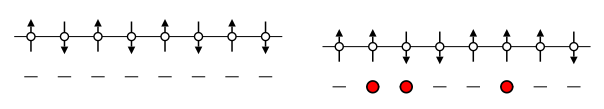
\includegraphics[scale=0.5]{fig1}
\caption{Соответствие между спинами $S = 1/2$ и бозонами для одномерной цепи.}
\label{}
\end{figure}

Причина использования этого отображения состоит в том, что с бозонами легче проводить вычисления из-за их более простых коммутационных соотношений. Теория линейных спиновых волн соответствует невзаимодействующим бозонам и по построению точна при $S \to \infty$. Результаты для конечного $S$ можно систематически улучшить, включив взаимодействия в форме $1 / S$-разложения. Здесь мы просто обрисовываем вычисления самого низкого порядка.
Если пренебречь ограничением, согласно которому число бозонов $n_i$ для каждого сайта должно быть в пределах $0, \dots , 2S$ (физическое подпространство), мы можем использовать следующее простое (низшего порядка по 1 / S) отображение между операторами спина в исходном гамильтониане (2) и операторами рождения и разрушения бозона $a_i^{+}$ и $a_i$ (и числовые операторы $n_i = a_i^{+}a_i$)
$i \in ↑$:
\begin{equation*}
 S_i^z=S-n_i 
\end{equation*}

\begin{equation*}
S_i^{+}=\sqrt{2S}a_i 
\end{equation*}

\begin{equation*}
S_i^{-}=\sqrt{2S}a_i^{+} 
\end{equation*}


$j \in ↓$:

\begin{equation}
 S_j^z=n_j-S 
\label{eq_4}
\end{equation}

\begin{equation*}
S_j^{+}=\sqrt{2S}a_j^{+} 
\end{equation*}

\begin{equation*}
S_i^{-}=\sqrt{2S}a_j 
\end{equation*}

Чтобы понять это отображение, полезно взглянуть на рис. 1 - помимо очевидного способа, которым недиагональные операторы могут влиять на состояния, нужно просто быть осторожным с различными факторами, связанными с рождением / разрушением бозонов и повышением спина. / понижение (обсуждается в стандартных текстах по квантовой механике). Множители в (~\ref{eq_4}) верны для $n_i << S$, но обратите внимание, что они также точны для $S = 1/2$ в физическом подпространстве. В принципе, можно записать более сложные выражения, которые формально верны для любых $S$ и $n_i$ в физическом подпространстве (а также автоматически разделяют физическое и нефизическое подпространства), но это актуально только при выходе за рамки линейной теории спиновых волн.

Теперь преобразуем слагаемые в гамильтониане (~\ref{eq_2}), используя отображение (~\ref{eq_4}). Поскольку мы рассматриваем двудольную систему, в которой два узла $i$ и $j$ всегда находятся на разных подрешетках, мы получаем недиагональный член

\begin{equation}
\frac{1}{2}(S_i^{+}S_j^{-}+S_i^{-}S_j^{+}) \longrightarrow (a_ia_j+a_i^{+}a_j^{+})
\label{eq_5}
\end{equation}

а диагональное взаимодействие равно:

\begin{equation}
S_i^{z}S_j^{z} \longrightarrow -S^2+S(n_i+n_j)-n_in_j
\label{eq_6}
\end{equation}

Теорию спиновых волн формально следует рассматривать как расчет с большим $S$. Поэтому в вычислениях самого низкого порядка мы должны отбросить член взаимодействия $n_i$ и $n_j$ в (~\ref{eq_6}), потому что он на $1 / S$ раз меньше, чем невзаимодействующие вклады из (~\ref{eq_5}) и (~\ref{eq_6}). Рассмотрим для определенности двумерную квадратную решетку с $N = L^2$ узлами. 

Запишем эффективный гамильтониан:
\begin{equation}
H = -2NS^2J+4SJ\sum\limits_{i=1}^Nn_i+SJ\sum\limits_{\langle ij \rangle} (a_ia_j+a_i^{+}a_j^{+})
\label{eq_7}
\end{equation}

Здесь следует отметить, что мы рассматриваем конечную систему, но предполагаем, что симметрия нарушена (направление разнесенной намагниченности заблокировано), что может быть строго истинным только в пределе $N \to \infty$ (если не добавлено какое-либо нарушающее симметрию поле к $H$). Однако это нормально, потому что мы в любом случае выберем предел $N \to \infty$ в конце.
Бозонный гамильтониан (~\ref{eq_7}) легко диагонализируется (т.е. записывается в терминах числовых операторов). Чтобы построить это решение, мы сначала применим преобразования Фурье,

\begin{equation}
a_k = N^{-\frac{1}{2}}\sum\limits_{\vec{r}}e^{i\vec{k}\vec{r}}a_{\vec{r}}
\label{eq_8}
\end{equation}

\begin{equation*}
a_r = N^{-\frac{1}{2}}\sum\limits_{\vec{r}}e^{-i\vec{k}\vec{r}}a_{\vec{k}}
\label{eq_8}
\end{equation*}

где операторы реального пространства были помечены их векторами координат решетки r, а не только индексом узла i, а импульс k находится в первой зоне Бриллюэна квадратной решетки (то есть обратной квадратной решетке из N узлов). \\

Тогда гамильтониан равен:

\begin{equation}
H = -2NS^2J+4SJ\sum\limits_{\vec{k}} n_{\vec{k}}+2SJ\sum\limits_{\langle ij \rangle} \gamma_{\vec{k}}(a_{\vec{k}}a_{\vec{-k}}+a_{\vec{k}}^{+}a_{\vec{-k}}^{+})
\label{eq_9}
\end{equation}

где, постоянная решетка устанавливаетя в 1 (т.е. $k_x,k_y=\frac{2n\pi}{L}, n \in {0,\dots,L-1}$),

\begin{equation}
\gamma_{\vec{k}} = \frac{1}{2}(cos(k_x)+cos(k_y))
\label{eq_10}
\end{equation}

Следующим шагом является преобразование Боголюбова в бозонные операторы, смешивающие исходные операторы $+\vec{k}$ и $−\vec{k}$;

\begin{equation}
\alpha_{\vec{k}} = cosh(\Theta_{\vec{k}})a_{\vec{k}}+sinh(\Theta_{\vec{k}})a_{-\vec{k}}^{+}
\label{eq_11}
\end{equation}

который имеет обратный вид:

\begin{equation}
a_{\vec{k}} = cosh(\Theta_{\vec{k}})\alpha_{\vec{k}}+sinh(\Theta_{\vec{k}})\alpha_{-\vec{k}}^{+}
\label{eq_12}
\end{equation}

Легко проверить, что операторы $\alpha_{\vec{k}}$ подчиняются стандартным бозонным коммутационным соотношениям для любого $\Theta_{\vec{k}}$. Особенность состоит в том, чтобы выбрать эти «углы» для каждого $\vec{k}$ так, чтобы все операторы $\alpha_{\vec{k}} \alpha_{\vec{-k}}$ и $a_{\vec{k}}^{+} a_{\vec{-k}}^{+}$ сокращаются в гамильтониане (~\ref{eq_9}). Это так, если

\begin{equation}
\frac{2cosh(\Theta_{\vec{k}})sinh(\Theta_{\vec{k}})}
{cosh^2(\Theta_{\vec{k}})+sinh^2(\Theta_{\vec{k}})}
=\gamma_{\vec{k}}
\label{eq_13}
\end{equation}

Преобразованный Боголюбов гамильтониан (гамильтониан спиновых волн) тогда диагонален по числам заполнения

\begin{equation}
H=E_0+\sum\limits_{\vec{k}}\omega_{\vec{k}}\alpha_{\vec{k}}^{+}\alpha_{\vec{k}}
\label{eq_14}
\end{equation}

константу можно записать как:

\begin{equation}
E_0 = -2SJ\sum\limits_{\vec{k}}\frac{\gamma_{\vec{k}}^2}{1+\sqrt{1-\gamma_{\vec{k}}^2}} - 2NS^2J
\label{eq_15}
\end{equation}

а дисперсионное соотношение в (~\ref{14}) для состояний спиновых волн $\alpha_{\vec{k}}^{+}|0\rangle$ имеет вид:

\begin{equation}
\omega_{\vec{k}}=4SJ\sqrt{1-\gamma_{\vec{k}}^2}
\label{eq_16}
\end{equation}

Для импульсов, близких к (0, 0) и ($\pi$, $\pi$), эта дисперсия линейна, $\omega_{\vec{k}}=ck$ и $\omega_{\vec{k}}=c|(\pi,\pi)-\vec{k}|$ соответственно со скоростью (скоростью спиновой волны) $c = 2\sqrt{2}SJ$.

Основное состояние  $|0\rangle$ в (~\ref{eq_14}) - это вакуум для спиновых волн, где энергия как раз равна $E_0$, определяемой (~\ref{eq_15}). Сумму можно вычислить численно, проще всего с помощью простого суммирование по импульсам на больших решетках и экстраполяция $E_0/N$ до $N \to \infty$ (или преобразование суммы, деленной на $N$, в интеграл, численное вычисление которого дает непосредственно значение $N \to \infty$). Результат будет $E_0/JN=-0,65795$ для $S=1/2$

Обратите внимание, что хотя основное состояние не содержит никаких $\alpha$-бозонов Боголюбова (спиновых волн), оно содержит некоторое количество исходных a-бозонов. Намагниченность подрешетки напрямую связана с плотностью этих бозонов, которая является однородной и может быть вычислена в любом узле или усреднена по узлам;

\begin{equation}
\langle m_s \rangle = S-\langle 0|a_i^{+}a_i|0 \rangle = S-\frac{1}{N}\sum\limits_{i=1}^N \langle 0|a_i^{+}a_i|0 \rangle
\label{eq_17}
\end{equation}

Используя преобразование Боголюбова, это становится:

\begin{equation}
\langle m_s \rangle = S-\frac{1}{N}\sum\limits_{\vec{k}} sinh^2(\Theta_{\vec{k}})
\label{eq_17}
\end{equation}

В наиболее интересном случае $S = 1/2$ это дает $\langle m_s \rangle = 0,3034$, или $\approx 61\%$ от «классического» значения $1/2$. Таким образом, квантовые эффекты (нулевые флуктуации, представленные наличием бозонов) уменьшают, но не разрушают дальний порядок.

В принципе неясно, должна ли теория спиновых волн быть надежной для малых $S$.
Этот вопрос много обсуждается, но на самом деле метод дает хорошее описание 2D-модели Гейзенберга на квадратной решетке. Несмещенные расчеты QMC дают результаты для $E_0$ и $\langle m_s \rangle$, отличающиеся от приведенных выше только на $1-2\%$. Это можно проследить апостериори до истинного значения $\langle m_s \rangle$, которое довольно большой (т.е. можно ожидать, что теория спиновых волн будет точной, когда плотность бозонов мала). В случаях, когда истинная намагниченность подрешетки мала или равна нулю, теория спиновых волн обычно работает не так хорошо, даже при переходе к более высоким порядкам в
1 / S (что очень сильно увеличивает сложность расчета ~\cite{prb_45_7127,prb_46_6276,prb_46_1_10763}).


\subsubsection{Разрушение порядка Нееля}
При выходе за пределы двудольных решеток с однородными взаимодействиями или путем дополнения модели Гейзенберга c дополнительными взаимодействиями (например, включающими более двух спинов) квантовые флуктуации могут стать настолько значительными, что основное состояние теряет свой дальний неелевский порядок (сохраняя только короткие - диапазон антиферромагнитных корреляций). Есть несколько других возможных типов упорядоченных и неупорядоченных основных состояний, некоторые из которых не имеют классических аналогов. В настоящее время большой интерес к квантовым спиновым моделям связан с существованием немагнитных состояний и квантовых фазовых переходов между ними и состоянием Нееля ~\cite{sachdev1}.  Одна важная причина для изучения таких переходов проистекает из купратных высокотемпературных сверхпроводников, нелегированные исходные соединения которых являются антиферромагнетиками, близко соответствующими слабосвязанным слоям Гейзенберга (многие свойства которых можно понять на основе одного слоя) ~\cite{rmp_63_1}. В этих системах магнитный порядок разрушается при легировании подвижными носителями заряда. Это очень сложная электронная задача многих тел, в которой вычислительные исследования также играют важную роль ~\cite{rmp_66_763,psj_76_113708,prb_79_220504}. В то время как полное решение проблемы высоких $T_c$, конечно, потребует более сложных моделей (возможно, некоторой разновидности $t-J$ или модели Хаббарда), некоторые общие аспекты физики, близкие к квантовому фазовому переходу из состояния Нееля, могут, однако , можно понять на основе спиновых моделей ~\cite{rmp_75_913}.

Помимо купратов и связанных с ними антиферромагнитных систем, существует также множество материалов с неоднородными или фрустрированными спиновыми взаимодействиями ~\cite{schol, diep, rmp_82}, которые могут приводить к немагнитным низкотемпературным состояниям. Многие из этих состояний и возможные количественные фазовые переходы между ними до сих пор недостаточно изучены. Поэтому полезно искать и изучать прототипы квантовых спиновых моделей, которые реализуют различные типы основных состояний и квантовых фазовых переходов. Исследования квантовых фазовых переходов также имеют более широкий контекст понимания «экзотических» проявлений квантовой механики на коллективном уровне многих тел ~\cite{sachdev1}. Есть даже интересные связи с физикой элементарных частиц - существуют близкие аналогии между фазовыми переходами в суперсимметричных калибровочных теориях в $2 + 1$ измерениях и «деконфайнтированными» квантово-критическими точками, которые могут разделять основные состояния 2D Нееля и VBS ~\cite{ap_325}.

\subsection{Спиновые жидкости и твердые тела с валентной связью}
В рамках теории линейных спиновых волн немагнитное состояние соответствует бозонной плотности $\langle n_i \rangle = S$. Этот вид состояния, однако, не является хорошим представлением реальных немагнитных основных состояний Гейзенберга и связанных с ним квантовых спиновых моделей, потому что это действительно так. Эти состояния не содержат корреляционных эффектов. Чтобы обсудить более интересные немагнитные состояния, полезно сначала взглянуть на квантовые флуктуации с другой точки зрения.

Для двух изолированных спинов $i$, $j$ (димер,$N = 2$) основным состоянием антиферромагнитного гамильтониана Гейзенберга $S = 1/2$ (~\ref{eq_1}) является синглет;

\begin{equation}
\langle \phi_{ij}^s \rangle = S\frac{|↑_i↓_j\rangle - |↓_i↑_j\rangle}{\sqrt 2}
\label{eq_19}
\end{equation}

Хотя два спина в таком синглете всегда идеально антикоррелированы (запутаны), отдельные спины сильно (максимально) флуктуируют, и статический порядок спинов отсутствует; $\langle \vec{S_i} \rangle = \langle \vec{S_j} \rangle = 0$.

 Напротив, идеальные состояния Нееля для $N = 2, |↑_i↓_j \rangle  и | ↓_i ↑_j \\rangle$, являются состояния произведения (то есть формы $|\phi_i \rangle \bigotimes |\phi_j \rangle$) без флуктуаций (и без запутывания, грубо говоря, степень запутанности соответствует отклонениям от состояния произведения). Стоит обратить внимание, что для $N = 2$ (собственная) энергия синглета составляет $-3J_{ij} / 4$, тогда как математическое ожидание энергии в состояниях Нееля намного выше, $-J_{ij}/4$ (и состояния не являются собственными состояниями). Тенденция взаимодействующих спинов к запутыванию путем образования парных синглетов для минимизации энергии сохраняется в многоспиновых системах, но когда $N> 2$, спин не может одновременно образовывать чистые синглетные пары со всеми своими соседями. Вместо этого систему можно рассматривать как суперпозицию различных синглетных пар. Тогда никакая пара не находится в чистом синглете, и поэтому вклад энергии от каждого взаимодействия $H_{ij}$ всегда выше, чем энергия синглета $-3J_{ij} / 4$. Это можно рассматривать как уменьшение квантовых флуктуаций (приводящие к менее чем максимальной двухспиновой запутанности) для $N> 2$, приближая состояние (или, вернее, матрицу плотности) каждой взаимодействующей пары к состоянию произведения. Состояние с антиферромагнитным дальним порядком, нарушающим орбитальную инвариантность гамильтониана может сформироваться в термодинамическом пределе, если имеется достаточно флуктуаций в синглетных парах (и нужно обратить внимание, что с точки зрения синглетов состояние Нееля имеет большие флуктуации, чем, например, состояние фиксированных синглетных спариваний, т.е. если быть точным, флуктуации всегда следует указывать относительно некоторого эталонного состояния). Если система является одномерной, или если взаимодействия сильно фрустрированы (конкурируют), или если геометрия решетки и связи способствуют образованию синглетов в определенной структуре (например, в системе слабосвязанных димеров), антиферромагнитный порядок может не присутствовать в основном состоянии при $N \to \infty$.

~\emph{Состояния валентной связи.}

Приведенную выше интуитивную картину состояния флуктуирующих синглетов на самом деле можно сделать строгой. Любое синглетное состояние может быть расширено до базисных состояний, которые являются продуктами синглетных пар или валентных связей. Обозначив $(i, j)$ синглет спинов $i$ и $j$, как в уравнении (~\ref{eq_19}) нормированное базисное состояние валентной связи для $N$ (четных) спинов имеет вид

\begin{equation}
\langle \phi \rangle = N^{-1/4}| (i_1,j_1)(i_2,j_2) \dots (i_{N/2}, j_{N/2}) \rangle
\label{eq_20}
\end{equation}

где каждый индекс позиции появляется ровно один раз (т.е. каждый спин принадлежит одному синглету).

Этот базис является переполненным в синглетном подпространстве, и, таким образом, любое синглетное состояние может быть расширено в эти состояния, но коэффициенты разложения не уникальны. Базис валентных связей и вычислительные методы, использующие его, обсуждаются в статьях ~\cite{prl_95_207203,npb_750,arXiv_0704_1469,prb_82_024407}. Здесь мы просто отметим, что некоторые типы состояний более естественно выражаются в базисе валентных связей, чем в стандартном базисе отдельных спинов ↑ и ↓.

Чтобы базис валентной связи был (сверх) полным, должна быть разрешена произвольная длина связей. Ограничение длины делает базис неполным (хотя на самом деле можно ограничить связи только для соединения сайтов на двух разных подрешетках). При некоторых типах состояний все еще полностью доминируют короткие связи (то есть вероятность связи длины r быстро убывает с r). Такие состояния с короткой связью в двух измерениях не имеют магнитного дальнего порядка (в то время как в трех измерениях они могут быть упорядочены по Неелю) и часто называются спиновыми жидкостями или состояниями резонирующей валентной связи (RVB). Различные типы кристаллического порядка могут также формироваться в конфигурациях связей, приводя к периодическим модуляциям в наблюдаемых величинах, таких как $\langle S_i S_j \rangle$ (где $i$, $j$ - позиции ближайших соседей). Такие упорядоченные состояния (которые нарушают симметрию решетки) называются твердыми телами с валентными связями (VBS) или кристаллами с валентными связями. Типичные конфигурации валентных связей в состояниях RVB и VBS показаны на рис.2.

\begin{figure}[htp]
\centering
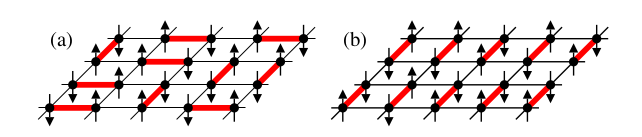
\includegraphics[scale=0.5]{fig2}
\caption{Состояния валентной связи в двух измерениях. Толстые линии - синглеты.}
\label{}
\end{figure}

\subsection{Одномерные системы}
Исследования квантовых спиновых цепочек - точное решение Бете модели Гейзенберга $S = 1/2$ ~\cite{ph_71} - решение очень сложное (часто требует сложных численных расчетов ~\cite{sm_2006, mp_59_091417}), многие свойства цепи Гейзенберга были получены лишь значительно позже дополнительные методы (в частности, ренормгрупповые трактовки эффективных низкоэнергетических теорий поля ~\cite{prl_50_1153, prl_55_1355, mpa_22_511, mpa_22_2562, prb_39_4620}

Как мы уже отмечали, в одномерной системе Гейзенберга не может быть магнитного порядка (но VBS-порядок разрешен, поскольку он нарушает дискретную симметрию). Функция спиновой корреляции $C(r) = \langle  S_i · S_{i + r} \rangle$ цепочки Гейзенберга убывает с расстоянием $r$ как $(−1)^r/ r$ (с мультипликативной логарифмической поправкой). Таким образом, основное состояние является критическим (или квазидальнодействующим, на грани упорядочения). Включение фрустрированного взаимодействия вторых ближайших соседей, когда оно достаточно сильное, вызывает квантовый фазовый переход в состояние VBS (иногда также называемое состоянием спин-Пирлса), где спиновые корреляции экспоненциально затухают с расстоянием ~\cite{mp_10_1388}.

Хотя квазиодномерные антиферромагнетики активно изучались экспериментально уже в 1960-х и 1970-х годах, эти усилия были дополнительно стимулированы теоретическими разработками в 1980-х годах. Холдейн предположил ~\cite{prl_50_1153} , основываясь на подходе теории поля, что цепочка Гейзенберга имеет совершенно разные физические свойства для целочисленного спина ($S = 1, 2, \dots $) и «полунечетного целого» спина ($S = 1 / 2, 3/2, \dots $). Из решения Безе было известно, что цепь $S = 1/2$ имеет бесщелевой спектр возбуждения (связанный со степенными затухающими спиновыми корреляциями). Холдейн предположил, что цепь $S = 1$ вместо
основное состояние с экспоненциально убывающими корреляциями и щелью для всех возбуждений; своего рода состояние спиновой жидкости ~\cite{cmp_115_477}. Это противоречило ожиданиям (основанным, например, на теории спиновых волн), что увеличение $S$ должно увеличивать тенденцию к упорядочению. Гипотеза Холдейна
стимулировал интенсивную исследовательскую деятельность, как теоретическую, так и экспериментальную, в области цепочки Гейзенберга $S = 1$ и одномерных систем в более широком смысле. В настоящее время численные исследования полностью убедительно свидетельствуют о том, что Холдейн был прав ~\cite{prb_40_2421, prl_64_1597, prb_54_4038}. Экспериментально существует также ряд квазиодномерных $S = 1/2$ ~\cite{prl_70_4003} и $S=1$ ~\cite{prb_50_9174} (а также более крупный $S$ ~\cite{prl_77_1616}) соединений, которые показывают предсказанные различия в спектре возбуждения. Возникла довольно полная и убедительная теория цепочек Гейзенберга со спином $S$ (включающая также VBS-переходы для получетного целого $S$), но даже до сих пор различные аспекты их необычных свойств все еще исследуются ~\cite{prl_96_257202}. Существует также множество других вариантов спиновых цепочек, которые также привлекают много теоретического и экспериментального внимания (например, системы, включающие различные анизотропии, внешние поля ~\cite{prl_95_077201}, взаимодействия более высокого порядка ~\cite{prb_74_144426}, связи с фононами ~\cite{prl_83_195, arXiv_0705_0799}), дальнодействующие взаимодействия ~\cite{sm_2005_P12001, prl_104_137204} и др.). Мы будем использовать методы точной диагонализации для исследования цепочки Гейзенберга $S = 1/2$.

\subsection{Модели с квантовыми фазовыми переходами в двух измерениях}
Существование различных типов основных состояний подразумевает, что фазовые переходы могут происходить в системе при $T = 0$ при изменении некоторого параметра в гамильтониане (что экспериментально может быть достигнуто в квантовых магнитах, например, как функция давления или внешнего магнитного поля) ~\cite{prl_100_205701} - следует, однако, отметить, что возможности более ограничены, чем в моделях). Как и в классических фазовых переходах, управляемых температурой, такие квантовые фазовые переходы могут быть непрерывными или первого рода, как показано на рис.3.

\begin{figure}[htp]
\centering
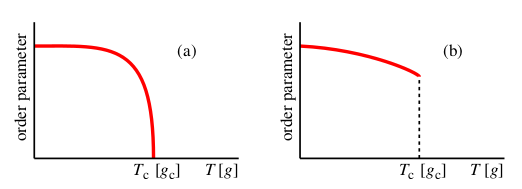
\includegraphics[scale=0.5]{fig3}
\caption{Температурная (T) или связная (g) зависимость параметра порядка (например, намагниченности ферромагнетика) при непрерывном (а) и фазовом переходе первого рода (б)}
\label{}
\end{figure}

Обычно фазовый переход связан с параметром порядка, который равен нулю в неупорядоченной фазе и отличен от нуля в упорядоченной фазе. например, намагниченность m ферромагнетика или намагниченность подрешетки $m_s$ антиферромагнетика. Существуют топологические фазовые переходы, не связанные с каким-либо локальным параметром порядка. Различные состояния при таких переходах различимы только по некоторой глобальной топологической величине ~\cite{Wen}.

В этом разделе мы вводим некоторые спиновые модели, демонстрирующие квантовые фазовые переходы в двух измерениях. Как мы уже видели, двумерная модель Гейзенберга $S = 1/2$ с взаимодействиями ближайших соседей имеет порядок Нееля при $T = 0$. Тогда возникает вопрос, как разрушить этот порядок и создать какое-то другое основное состояние.

\subsubsection{Димеризованные системы}
Возможно, самый простой способ получить немагнитное основное состояние 2D-модели Гейзенберга - это димеризовать систему ~\cite{prl_61_2484}, т.е. ввести слабые и сильные антиферромагнитные связи (связи), $J_1> 0$ и $J_2> J_1> 0$, соответственно, в такой схеме, что каждый спин принадлежит ровно одной сильной связи. Есть несколько способов сделать это, три из которых показаны на рис. 4. 

\begin{figure}[htp]
\centering
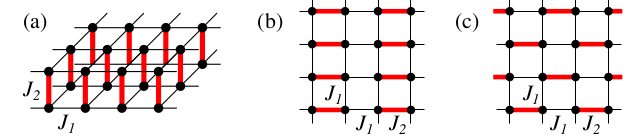
\includegraphics[scale=0.5]{fig4}
\caption{Димеризованные системы с двумя разными значениями силы связи между ближайшими соседями; бислой (а) с димерами поперек слоев и одиночные слои с столбчатыми (б) и шахматными (в) димерами.}
\label{}
\end{figure}

Когда $J_1 = 0$, эти системы состоят из $N/2$ независимых пар спинов (димеров) с внутридимерным взаимодействием $J_2$, и, как мы уже обсуждалось, основное состояние каждой такой пары - синглет; таким образом, основное состояние всей системы - состояние синглетного произведения (валентной связи), которое явно не имеет магнитного порядка. С другой стороны, при $J_2 = J_1$ основное состояние имеет порядок Нееля. Тогда возникает вопрос, как развивается основное состояние в зависимости от коэффициента связи $g = J_2 / J_1$. Возможно, предположить, что после связывания димеров должен появиться некоторый порядок Нееля, т.е. для любого $g < \infty$.

Однако оказывается, что фазовый переход действительно имеет место при некотором критическом значении g c (которое зависит от расположения димеров). Хотя этот переход может быть проанализирован с использованием нескольких аналитических и численных подходов, масштабирование данных QMC конечного размера в настоящее время является единственным способом получения несмещенных количественных результатов (например, ~\cite{prb_52_3521}, где обсуждается, как теория спиновых волн распадается на фазовый переход).

\begin{figure}[htp]
\centering
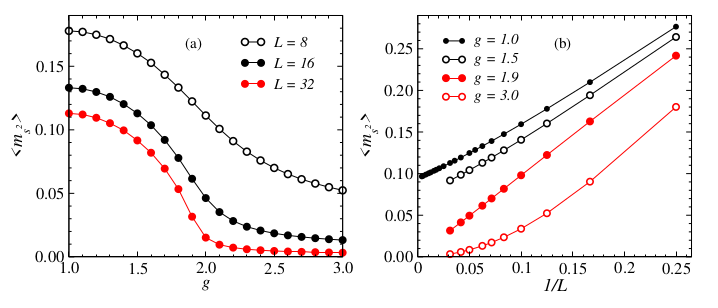
\includegraphics[scale=0.5]{fig5}
\caption{Результаты QMC для квадрата намагниченности подрешетки в двумерной модели Гейзенберга со столбчатой димеризацией. (а) показывает результаты в зависимости от коэффициента связи $g$ для разных размеров решетки, а (б) показывает зависимость от размера для нескольких значений $g$. Квантовый фазовый переход, при котором неелевский порядок исчезает, происходит при $g ≈ 1.9$.}
\label{}
\end{figure}

На рис. 5 показаны некоторые результаты QMC для столбчатой модели димера на рис. 4 (б). Параметр порядка - это ступенчатая намагниченность, с соответствующим оператором, определенным в формуле. (~\ref{eq_3}). Это векторный оператор, и для конечной решетки его математическое ожидание обращается в нуль из-за спин-орбитальной симметрии гамильтониана. Его площадь, $\langle m_s^2 \rangle$, была вычислена в ходе моделирования. На рис. 5 (a) показаны результаты для решеток $L × L$ в зависимости от коэффициента связи g, а на рис. 5 (b) показаны данные для нескольких значений g в графическом виде в зависимости от $1 / L$ (что часто является наиболее удобным способом графического представления данных, когда исследуя сходимость к ненулевому значению при $L \to \infty$). Здесь видно, что поведение меняется при $g \approx 1.9$; ниже этой связи намагниченность подрешетки экстраполируется до ненулевого значения в термодинамическом пределе, тогда как при больших $g$ она спадает до нуля.

Важным вопросом, касающимся квантового фазового перехода в димеризованных системах, является его класс универсальности. Квантовая система многих тел в $d$-измерениях может быть формально отображена с помощью интегралов по траекториям в эффективную классическую систему в $2 + 1$ измерениях. Многие свойства были предсказаны таким образом на основе ренормгрупповой трактовки. Пример нелинейной $\sigma$ -модели в $2 + 1$ измерениях - ~\cite{prb_39_2344, prb_49_11919}. Основываясь только на аргументах симметрии, можно было бы ожидать, что переход будет в классе универсальности трехмерной классической модели Гейзенберга. Однако в квантово-классическом отображении есть тонкие проблемы, и поэтому для проверки различных предсказаний необходимо моделирование QMC. Результаты по переходу в двухслойной (а) ~\cite{prb_73_014431} и столбчатой ​​димерной (б) системе ~\cite{prb_65_014407}  системе на рис. 4 (и некоторых других случаях ~\cite{prl_76_3822, prb_79_014410}) хорошо согласуются с ожиданиями, недавние исследования димеров в шахматном порядке (c) и показывают неожиданные отклонения в ~\cite{prl_101_127202}, которые до сих пор не изучены.

\subsubsection{Фрустрированные системы}
Типичным примером фрустрации является система с антиферромагнитными взаимодействиями на треугольной решетке. Если сначала взглянуть на эту проблему в рамках модели Изинга, то спины одного треугольника не могут одновременно быть антипараллельными обоим своим соседям - существует шесть конфигураций с минимальной энергией, и все они имеют одну «фрустрированную» связь (два параллельных соседа), как показано на рис. 6. Поскольку это является следствием решетки, это часто называют геометрическим расстройством. При увеличении размера системы вырождение основного состояния растет с увеличением размера системы, и в ансамбле среди всех этих конфигураций нет никакого порядка ~\cite{mp_11_413, mg_15_L631}. Однако в случае классической модели $XY$ (плоский вектор) или модели Гейзенберга (трехмерные векторы) порядок существует при $T = 0$ (но не при $T> 0$, согласно теореме Мермина-Вагнера).
Энергия минимизируется путем расположения спинов в плоскости под углом $120^\circ $ по отношению к их соседям в том же треугольнике, как показано для единственного треугольника на рис. 6. Это состояние называется трехподрешеточным состоянием Нееля. Вариант $S = 1/2$ этой модели был исследован во многих случаях. Фактически это была система, для которой первоначально было предложено спин-жидкостное состояние RVB ~\cite{pm_30_23}. Однако сейчас есть убедительные численные доказательства того, что трехподрешеточный порядок Нееля действительно выживает при квантовых флуктуациях ~\cite{prb_50_10048, prl_99_127004}.

\begin{figure}[htp]
\centering
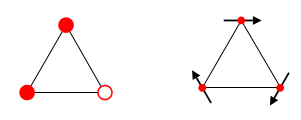
\includegraphics[scale=0.5]{fig6}
\caption{Изинговская (слева) и планарная (справа) спиновые конфигурации с минимальной энергией на треугольнике с антиферромагнитными взаимодействиями ближайших соседей.}
\label{}
\end{figure}

На квадратной решетке эффекты фрустрации можно исследовать, добавляя взаимодействия за пределами ближайших соседей. Хорошо изученным случаем является модель $J_1 -J_2$, где $J_1$ и $J_2$ относятся, соответственно, к силе взаимодействий между ближайшими и следующими ближайшими соседями. В система расстраивается, если оба $J_1> 0$, $J_2> 0$ или если $J_1 <0$, $J_2> 0$. Даже со спинами Изинга это весьма нетривиальная система с нерешенными вопросами, которые все еще вызывают интерес ~\cite{pre_80_051117, phys_145_012051, prl_108_045702}. 
В случае квантовых спинов, модель Гейзенберга $S = 1/2$ $J_1-J_2$ со всеми антиферромагнитными связями является одной из прототипов моделей с квантовым фазовым переходом из стандартного состояния Нееля, в данном случае в зависимости от коэффициент связи $g = J_2 / J_1$.
Хотя многие различные расчеты довольно последовательно показывают, что порядок Нееля исчезает при критическом отношении связи $gc ≈ 0,4$ ~\cite{prl_63_2148, phys_6_675, prb_60_7278, prb_63_104420, el_74_896, prb_79_224431, prb_79_024409}, порядок фазового перехода и природа немагнитного основного состояния все еще вызывает споры. Большинство исследований указывают на некоторый тип состояния VBS, причем столбчатое состояние является первым кандидатом, но также было предложено состояние спиновой жидкости RVB ~\cite{prl_87_097201}.
При больших $g$, выше $g ≈ 0,6$, снова возникает магнитный порядок. Это можно понять в пределе $g \to \infty$, когда система распадается на два отдельных антиферромагнетика Гейзенберга с квадратной решеткой. При $g = \infty$ ($J_1 = 0$) относительное направление в пространстве спинов антиферромагнитного порядка внутри этих подсистем произвольно, но для любого $J_1> 0$ подсистемы сцепляются друг с другом и образуют коллинеарный спиновый порядок с вертикальными или горизонтальными полосами параллельных спинов (состояние, нарушающее симметрию вращения решетки на $90^\circ$ в дополнение к симметрии глобального вращения спина). Переход между немагнитным и коллинеарным состояниями, скорее всего, является переходом первого рода.

\begin{figure}[htp]
\centering
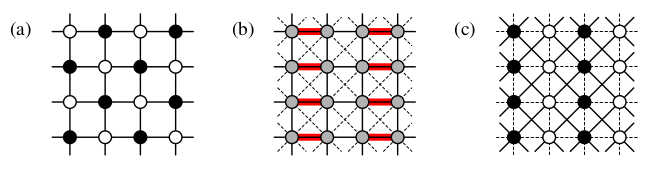
\includegraphics[scale=0.5]{fig7}
\caption{
Модель Гейзенберга с квадратной решеткой $S = 1/2$ с взаимодействием только ближайших соседей $J_1> 0$ имеет антиферромагнитное основное состояние, на рисунке (а) показано светлыми и сплошными кружками для $\langle S_i^z \rangle > 0$ и $\langle S_i^z \rangle <0$. В (б) взаимодействия следующих ближайших соседей J 2> 0 показаны пунктирными линиями. Когда $0,4 <J_2 / J_1 <−0,6$ (приблизительно), основное состояние может быть столбчатым VBS, с $\langle S_i^z \rangle =0$ на всех позициях, но с модуляциями в корреляциях связей $\langle S_i S_j \rangle$ (где i, j являются ближайшими соседи), как показано более толстыми линиями для более сильно коррелированных связей, образующих столбчатый узор. Для $J_2 / J_1> 0,6$ основное состояние имеет коллинеарный (полосатый) магнитный порядок, как показано на (c).}
\label{}
\end{figure}

Три различных основных состояния модели Гейзенберга $J_1-J_2$ со спинами $S = 1/2$ показаны на рис. 7. Классическая версия этой модели (Изинга, XY или Гейзенберга) имеет прямое (первого - порядка) Неелевский-коллинеарный переход $T = 0$ точно при $g = 1/2$ (что можно легко проверить, просто вычислив энергии этих состояний для $g <1/2$ и $g> 1/2$).
Таким образом, магнитно-неупорядоченное состояние индуцируется квантовыми флуктуациями и не имеет прямого классического аналога. Неясно, сохраняется ли такое состояние для $S = 1$ или более высоких спинов - для некоторого большого S, возможно, уже $S = 1$, оно должно уступить место переходу Нееля-Коллинеара первого рода, как в классической системе.

Причина, по которой было так трудно прийти к твердому выводу о природе немагнитного состояния и квантовом фазовом переходе между ним и состоянием Нееля, заключается в том, что крупномасштабная модель несмещенных вычислительных исследований $S = 1/2$ $J_1 -J_2$ в настоящее время невозможна из-за «проблем со знаком», влияющих на расчеты QMC фрустрированных систем.
Нет другого несмещенного метода, который может достичь достаточно больших решеток, например, точная диагонализация может достигать только $N ≈ 40$ спинов.

\subsubsection{Класс моделей J-Q}
VBS-состояния квантовых спиновых систем в двух измерениях были теоретически предсказаны достаточно давно ~\cite{prl_62_1694}. Формирование VBS связано со спонтанно нарушенной трансляционной симметрией решетки. Таким образом, состояние VBS и квантовые фазовые переходы в него сильно отличаются от немагнитных состояний и переходов в димеризованных «вручную» системах. Хотя в обоих случаях существует модель «сильных» и «слабых» спиновых корреляций, квантовые флуктуации в системах с нарушенной вручную и спонтанно нарушенной трансляционной симметрией различны (что гораздо интереснее в состояниях VBS). До недавнего времени крупномасштабные вычислительные исследования состояний VBS и квантовых фазовых переходов Нееля-VBS не проводились, начиная с микроскопических гамильтонианов, из-за проблем со знаком QMC, влияющих на фрустрированные модели Гейзенберга (которые на первый взгляд являются наиболее естественными системами, в которых для изучения физики немагнитных состояний).

Состояния VBS и переход Néel-VBS вновь привлекли внимание с предложением ~\cite{sc_303_1490}, что этот переход обычно является непрерывным и, таким образом, нарушает «правило Ландау», согласно которому переход порядок-порядок (между состояниями, нарушающими несвязанные симметрии) должен быть первого порядка (за исключением точно настроенных мультикритических точек).
В сценарии квантовой критичности «деконфайндер» параметры порядка VBS и Нееля являются проявлением удержания спинонов и конденсации соответственно. Спиноны можно рассматривать как $S = 1/2$ степеней свободы, но они соответствуют не только голым отдельным спинам на узлах решетки, но и более сложным коллективным объектам, «одетым» взаимодействиями. Некомпактная теория поля CP$^1$ была предложена для описания таких спинонов, связанных с возникающим калибровочным полем (в котором существуют спиноны) ~\cite{sc_303_1490}. Тогда центральный вопрос заключается в том, действительно ли эта низкоэнергетическая физика континуальной теории поля может возникнуть, исходя из разумного микроскопического гамильтониана. Ответ на этот вопрос требует крупномасштабных вычислительных исследований моделей, демонстрирующих переходы Нееля-VBS.

Поскольку проблема знака QMC запрещает крупномасштабные исследования модели $J_1 -J_2$ Гейзенберга и других подобных фрустрированных систем, принимаются попытки попробовать что-то еще. В классе моделей «J-Q» ~\cite{prl_98_227202, prb_80_180414, prb_82_174428} порядок Нееля разрушается взаимодействием (Q), которое не фрустрировано в стандартном смысле, но все же конкурирует с взаимодействием Гейзенберга (J). Чтобы понять эти модели J-Q, стоит обратить внимание, что взаимодействие Гейзенберга с точностью до константы равно оператору синглетного оператора: $H_{ij} = −S_{ij} + \frac{1}{4}$, где

\begin{equation}
S_{ij} = \frac{1}{4}-S_iS_j
\label{eq_20}
\end{equation}

Пара-синглет, уравнение (~\ref{eq_19}) является собственным состоянием этого оператора с собственным значением 1, тогда как триплетное состояние им разрушается;

\begin{equation*}
S_{ij}|\phi_{ij}^s\rangle = |\phi_{ij}^s\rangle
\end{equation*}

\begin{equation}
S_{ij}|\phi_{ij}^{t,m}\rangle = 0
\label{eq_23}
\end{equation}

\begin{equation*}
m=0, \pm 1
\end{equation*}

Таким образом, когда $S_{ij}$ действует на синглет-триплетную суперпозицию, выживает только синглетный компонент («проецируется наружу» - обратите внимание, что свойство $S_{ij}^2 = S_{ij}$, требуемое для оператора проекции, выполняется). Таким образом, стандартное гейзенберговское взаимодействие способствует образованию синглетов на парах ближайших соседних узлов, но,  флуктуации этих синглетов среди множества различных пар спинов приводят к неелевскому порядку в основном состоянии. Идея моделей J-Q состоит в том, чтобы проецировать синглеты на два или более порядка коррелированным образом, используя произведения нескольких операторов $S_{ij}$ на подходящий набор разных связей. Это способствует более высокой плотности коротких валентных связей, тем самым уменьшая или полностью разрушая антиферромагнитный порядок.

Исходный гамильтониан J-Q [~\ref{eq_17}] на квадратной решетке можно записать как

\begin{equation}
H=-J\sum\limits_{\langle ij \rangle} S_{ij} - Q \sum\limits_{\langle ijkl \rangle}S_{ij}S_{kl}
\label{eq_23}
\end{equation}

где оба члена J и Q показаны на рис. 8. 

\begin{figure}[htp]
\centering
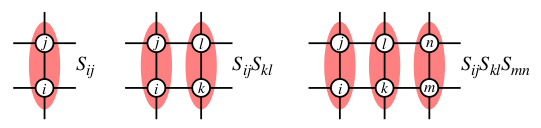
\includegraphics[scale=0.5]{fig8}
\caption{Графическое представление возможных конфигураций произведений  синглет-операторов $S_{ij}$ в J-Q-модель и ее обобщения. (а) - обмен Гейзенберга, (б) четырехспиновый взаимодействие исходной модели $J-Q$, и (c) взаимодействие с шестью спинами, которое приводит к более устойчивому порядку VBS. Эти операторы и их аналоги с поворотом на $90^\circ$ суммируются по всем позициям квадратной решетки.}
\label{}
\end{figure}

Также рассмотривают торы, расположенные на решетке различным (не столбчатым) образом ~\cite{prb_82_174428}[109]. При $J> 0$ и $Q> 0$ [со знаком минус перед взаимодействиями в уравнении (~\ref{eq_23})], коррелированные синглеты предпочтительны на элементах решетки, образованных продуктом синглетных проекторов. Только из гамильтониана все еще не ясно, реализуется ли состояние VBS при больших Q / J - поскольку гамильтониан не нарушает никаких симметрий (взаимодействия на рис. 8 суммируются по всем отдельным сдвигам и поворотам решетки), состояние VBS формируется только в том случае, если гамильтониан также содержит в себе неявно некоторые эффективные взаимодействия, которые благоприятствуют синглетам в некотором упорядоченном образце. Модель J-Q (~\ref{eq_23}) действительно демонстрирует переход Нееля-ВБС при $Q_c / J \approx 22$ ~\cite{prl_98_227202, prb_80_180414, prl_104_177201} и при более низком $Q_c$, если используется более двух синглетных проекторов ~\cite{prb_80_180414, prb_82_174428}.

~\emph{Параметры порядка. }

В качестве альтернативы квадрату полной пространственно усредненной намагниченности подрешетки (~\ref{eq_3}) обнаруживается наличие или отсутствие порядка Нееля с помощью спиновой корреляционной функции,

\begin{equation}
С(\vec{r_{ij}}) = \langle S_iS_j \rangle
\label{eq_24}
\end{equation}

на дальние расстояния рис. 9 (а) показаны результаты модели $J-Q$ для наибольшего разделения спинов, $\vec{r_{max}} = (L / 2, L / 2)$, на периодических решетках $L × L$. Результаты должны быть тщательно проанализированы, чтобы определить точку перехода, но уже эти необработанные данные предполагают, что порядок Нееля исчезает, то есть $C(r_{max}) → 0$, когда $L → ∞$, для $J / Q <0,04$.

\begin{figure}[htp]
\centering
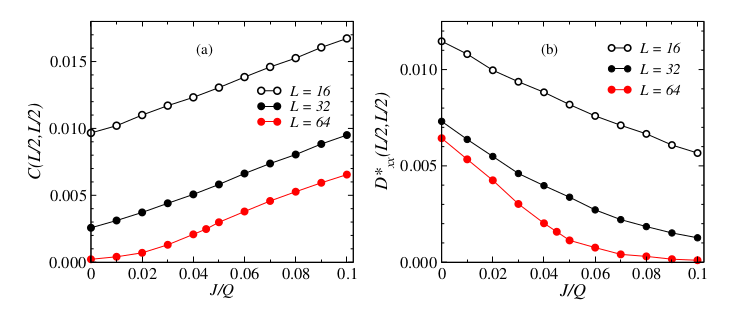
\includegraphics[scale=0.5]{fig9}
\caption{Результаты QMC для корреляционных функций дальнего спина (a) и шахматного димера (b) (соответствующих порядку Нееля и VBS соответственно) в основном состоянии модели $J-Q$ (23) в зависимости от отношения связи $J / Q$. Тщательный анализ этих корреляционных функций, а также других величин, указывает на единственную критическую точку $(J / Q)_c \approx 0,045$ , где и порядок Нееля, и порядок VBS непрерывно исчезают.}
\label{}
\end{figure}

Порядок VBS может быть обнаружен в корреляционной функции димера (или связи), определяемой как

\begin{equation}
D_{xx}(\vec{r_{ij}}) = \langle B_x(\vec{r_i})  B_x(\vec{r_j}) \rangle
\label{eq_25}
\end{equation}

где оператор облигации дается выражением

\begin{equation}
B_x(\vec{r_i}) = \vec{S}(\vec{r_j}) \vec{S}(\vec{r_i} + \hat{x})
\label{eq_26}
\end{equation}

Здесь вместо использования индекса $i$ в операторе спина для некоторой произвольной разметки узлов удобнее использовать соответствующий вектор положения решетки $\vec{r_i}$. Тогда $\vec{r}_i + \hat{x}$ соответствует позиции сразу после $\vec{r}_i$ в положительном направлении x. Индексы $xx$ в (25) указывают, что оба оператора связи $B_x$ ориентированы в направлении x, и эта корреляционная функция по симметрии равна $D_{yy}$ на решетке $L × L$. Можно также рассмотреть связи связей $D_{xy}$, где два оператора связи ориентированы по-разному. В состоянии VBS, таком как показанное на рис. 7, ожидается, что $D_{xx}(\vec{r})$ будет демонстрировать столбчатый узор меньших и больших значений. Затем параметр порядка VBS может быть определен как подходящее различие между этими модулированными корреляциями, например,

\begin{equation}
D_{xx}^{*}(\vec{r}) = D_{xx}(\vec{r})-\frac{1}{2}[D_{xx}(\vec{r} - \hat{x}) + D_{xx}(\vec{r}+\hat{x})]
\label{eq_27}
\end{equation}

Эта корреляционная функция показана на рис. 9 (б) при наибольшем разделении решетки для нескольких различных размеров системы. Здесь ясно, что порядок VBS существует для $J = 0$, вплоть до $J / Q \approx 0,04$, примерно там, где устанавливается порядок Нееля. Все расчеты до сих пор указывают на единственную критическую точку без какой-либо промежуточной третьей фазы или области
сосуществование порядка Néel и VBS.

\section{Классические фазовые переходы, моделирование методом Монте-Карло, конечное масштабирование}
Многие аспекты квантовых фазовых переходов и способы их анализа на основе численных данных о конечной решетке очень похожи на классические фазовые переходы. Здесь мы обсудим этот общий формализм в более простом контексте классических фазовых переходов, прежде чем перейти к расчетам и анализу данных для квантовых систем.
В классической статистической механике прототипом системы с непрерывным фазовым переходом является 2D-ферромагнетик Изинга, точное решение ~\cite{pr_65_117,Baxter} которого строго показывает, что такой фазовый переход существует. 

Эта модель определяется

\begin{equation}
E_\sigma = -J\sum\limits_{\langle ij \rangle}\sigma_i \sigma_j - h\sum\limits_{j=1}^N \sigma_i
\label{eq_28}
\end{equation}

которая представляет собой (потенциальную) энергию как функцию спинов $\sigma_i= \pm 1$. Мы используем $\sigma$ для общего обозначения всей спиновой конфигурации; $\sigma = (\sigma_1, \dots,\sigma_N)$. Поскольку связи взаимодействия $\langle ij \rangle$ ограничены ближайшими соседями на простой 2D квадратной решетке, точная критическая температура для бесконечной системы $T_c/J = 2 / ln (1 + \sqrt 2) \approx 2,269 $.
 Параметром порядка является намагниченность $\langle m \rangle = \langle \sigma_i \rangle $. 
 Он имеет асимптотический вид $T → T_c (T <T_c)$ форма $m ~ |t|^\beta$, где $t$ - приведенная температура, $t = (T - T_c) / T_c$, а показатель $\beta = 1/8$. Такие критические показатели и другие аспекты масштабного поведения при непрерывных фазовых переходах будут обсуждаться в этом разделе.

Точное решение модели Изинга очень особенное, и обычно фазовые переходы изучаются другими способами. Критические показатели появляются уже в простых теориях среднего поля, но их значения обычно неверны. Тем не менее теория среднего поля необходима как отправная точка, которую мы здесь обрисовываем для модели Изинга. Наиболее важной теоретической основой для фазовых переходов является ренормализационная группа, которая объясняет, как могут возникнуть универсальные (зависящие только от симметрии и размерности, а не от деталей взаимодействий) нетривиальные показатели (т.е. отличные от общих значений среднего поля,  ~\cite{cardy}). Для вычисления критических показателей и других свойств обычно используется моделирование методом Монте-Карло, при котором спиновые конфигурации выбираются стохастически в соответствии с распределением Больцмана. В этом разделе излагаются основы моделирования методом Монте-Карло (подробнее ~\cite{Landau_Binder, Newman_Barkema}). 

\subsection{Теория среднего поля модели Изинга}
В теориях среднего поля окружение подсистемы бесконечной решетки заменяется внешним полем, представляющим средние взаимодействия между подсистемой и окружающей средой. Подсистема может представлять собой одиночный спин или кластер из нескольких спинов. Здесь мы просто рассмотрим простейший случай расчета одного спина для модели Изинга, т.е. бесконечное окружение одного спина заменяется эффективным полем.

Гамильтониан (~\ref{eq_28}) удобно записать в расширенном виде с общими взаимодействиями $J_{ij}$ между всеми спинами (на произвольной решетке), а также с учетом внешнего магнитного поля;

\begin{equation}
E_\sigma = -\frac{1}{2}\sum\limits_{i=1}^N\sum\limits_{j=1}^N J_{ij}\sigma_i\sigma_j - h\sum\limits_{j=1}^N \sigma_i
\label{eq_29}
\end{equation}

Множитель $1/2$ компенсирует включение каждой взаимодействующей пары в сумму дважды (и $J_{ii} = 0$). Не накладывается никаких ограничений на знаки и величины $J_{ij}$, но для простоты предполагаем, что при наличии фазового перехода упорядоченное состояние является ферромагнитным. Чтобы построить и обосновать приближение одинарного спина, сначала группируются вместе все взаимодействия в (~\ref{eq_29}) с произвольным спином $i$;

\begin{equation}
E_i = -\sigma_i(\sum\limits_{j}J_{ij}\sigma_j+h)
\label{eq_30}
\end{equation}

Здесь нет множителя $1/2$ перед суммой, и мы использовали $J_{ij} = J_{ji}$.

Теперь предположим, что $h> 0$, так что $m = \langle \sigma_i \rangle> 0$. Мы будем исследовать спонтанное упорядочение в отсутствие поля, в конечном итоге позволив $h → 0$. Добавляя и вычитая константу, мы можем записать члены в круглых скобках в (30) как

\begin{equation}
\sum\limits_jJ_{ij}\sigma_j+h = m \sum\limits_{j}J_{ij}+h+\sum\limits_{j}J_{ij}(\sigma_j-m)
\label{eq_31}
\end{equation}

В своей самой основной формулировке теория среднего поля сводится к пренебрежению второй суммой в (~\ref{eq_31}) - флуктуационным членом, - после чего остается легко решаемая проблема одного спина в эффективном магнитном поле с напряженностью $J_sm + h$ ;

\begin{equation}
E_\sigma=-(J_sm+h)\sigma
\label{eq_32}
\end{equation}

где $J_s$ - сумма исходных связей

\begin{equation}
J_s=\sum\limits_jJ_{ij}
\label{eq_33}
\end{equation}

и мы предполагаем трансляционно-инвариантную систему, так что эта сумма не зависит от $i$. Намагниченность $m$ в (~\ref{eq_32}) на данном этапе неизвестна и будет определяться с помощью условия самосогласования; $\langle \sigma \rangle = m $.

\begin{equation}
\delta_m = \frac{\langle | \sum_jJ_{ij}(\sigma_j-m)| \rangle}{J_sm+h} << 1
\label{eq_34}
\end{equation}

Здесь $\langle \rangle$ обозначает математическое ожидание при фактическом распределении вероятностей (распределении Больцмана) спинов, которое мы не можем вычислить точно. В принципе флуктуации также могут быть рассчитаны в рамках теории среднего поля в качестве проверки внутренней согласованности. Даже не делая никаких вычислений, мы можем приблизительно вывести условия, при которых $\delta_m$ будет малым. Ясно, что $\delta_m$ мало, если есть существенный порядок, т. е. когда $(1 - m) = (1 - \langle \sigma_j\rangle) << 1$  потому что тогда больше всего $\sigma_j=1 \approx m$. Это так, если $h$ велико. Это также верно для $h = 0$, если симметрия спонтанно нарушена, и $m$ близко к $1$, т. е. при $T << T_c$, если есть фазовый переход.

Кроме того, $\delta_m$ может быть малым даже если $m$ не очень велико, если сумма по $j$ включает в себя множество ненулевых (и относительно больших) констант связи $J_{ij}$ - из-за подавления флуктуаций сумма $\sum_jJ_{ij}\sigma_j$ обычно (в большинстве случаев статистически важные спиновые конфигурации) близки к $m\sum_jJ_{ij}$. 
В крайнем случае однородных взаимодействий с бесконечным радиусом действия, $J_{ij} = J / N$ для всех $i, j$ и $N → ∞$ (где мы рассматриваем $J$ как конечную константу, например, $J = 1$, чтобы иметь конечную энергию ) все флуктуации точно сокращаются и $\delta_m = 0$ (и тогда теория среднего поля точна). 
В точности это верно и для короткодействующих взаимодействий на бесконечномерной решетке. Таким образом, в общем, даже если $m$ невелико, можно ожидать, что мера флуктуации $\delta_m$ будет мала для систем больших размеров и / или для дальнодействующих взаимодействий. Это те условия, при которых можно ожидать количественной точности теории среднего поля. Даже в тех случаях, когда она не является количественно точной, теория среднего поля может дать ценную информацию качественно.

Решим теперь фактически задачу среднего поля (~\ref{eq_32}), т.е. задачу одинарного спина (~\ref{eq_32}) при условии самосогласования $\langle \sigma \rangle = m$. 

Намагниченность равна

\begin{equation}
\langle \sigma \rangle = \frac{\sum\limits_\sigma\sigma e^{\sigma(J_sm+h)/T}}{\sum\limits_\sigma e^{\sigma(J_sm+h)/T}} = tanh[(J_sm+h)/T]
\label{eq_35}
\end{equation}

и поэтому условие самосогласованности читается как

\begin{equation}
m = tanh[(J_sm+h)/T]
\label{eq_36}
\end{equation}

Это уравнение, как правило, необходимо решать численно, что можно легко сделать, используя последовательные скобки для решения. Для малых m и h мы можем продолжить аналитически, расширив до ведущего порядка по m, h. Во-первых, когда внешнее поле $h = 0$, $m = 0$ является решением для всех $T$. В поисках других возможных решений, расширяя (~\ref{eq_36}) до третьего порядка по $x = J_s m + h$, $tanh (x) = x - x^3/3$, мы имеем

\begin{equation}
m^2 = 3 \frac{T^2}{J_s^2}\frac{J_s-T}{J_s}
\label{eq_37}
\end{equation}

по которой мы можем определить критическую температуру $T_c = J_s$, ниже которой намагниченность может быть отличной от нуля. Асимптотическое поведение $T → T_c$ равно

\begin{equation}
m=(3\frac{T_c-T}{T_c})^{1/2}, (h=0, T<T_c)
\label{eq_38}
\end{equation}

Из (~\ref{eq_36}) можно также получить полевую зависимость намагниченности при $T_c$ при $h → 0$.
Сохраняя старшие члены по $h$ разложения третьего порядка при $T = J_s$, получаем

\begin{equation}
m=(3\frac{h}{J_s})^{1/3}, (T=T_c)
\label{eq_39}
\end{equation}

Поучительно также посмотреть на полное численное решение для m. На рис. 10 (а) показаны некоторые примеры полевой зависимости m при различных температурах. При $T> T$ c поведение аналитически при $h = 0$, с особенностью, описываемой (39), развивающейся при $T → T_c$.
Ниже $T_c$ поведение прерывистое, что соответствует переходу первого рода в зависимости от $h$ между состояниями $m <0$ и $m> 0$. Разрыв соответствует спонтанной намагниченности в нулевом поле, полное численное решение которой представлено на рис. 10 (b), а асимптотика $T → T_c$ - поведение которой задается формулой (38). Здесь роль $h → 0^{+}$ или $h → 0^{-}$ в вычислении состоит в том, чтобы нарушить вырождение между $\pm m$ решениями. Вырождение при $h = 0$ также соответствует сосуществованию двух упорядоченных состояний точно при переходе первого рода.

\begin{figure}[htp]
\centering
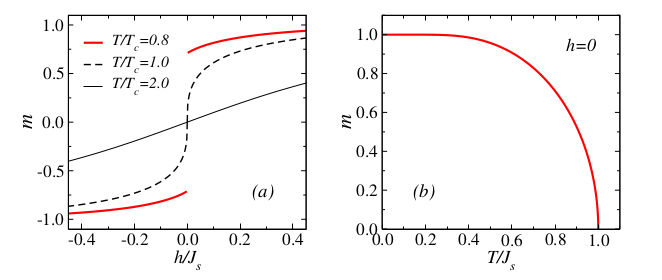
\includegraphics[scale=0.5]{fig10}
\caption{Среднее поле модели Изинга. (а) Зависимость намагниченности от внешнего поля для температур выше, при и ниже T c. Разрыв при h → 0 + и h → 0 - соответствует спонтанной намагниченности при h = 0. (б) Температурная зависимость спонтанной намагниченности.}
\label{}
\end{figure}

Перенося результат $T_c = J_s$ на $J_s$, указанный в уравнении. (33) дает $T_c = 4J$ для 2D-модели Изинга с взаимодействием ближайших соседей силой J. Это намного выше правильного значения, $T_c/J \approx 2,269$. Можно ожидать завышенной оценки $T_c$ из-за пренебрежения флуктуациями (которые, естественно, снижают $T_c$).

Показатели $\beta = 1/2$ и $\delta = 1/3$ в (~\ref{eq_38}) и (~\ref{eq_39}) в общем случае являются значениями этих критических показателей в рамках теорий среднего поля. Другие показатели также могут быть вычислены ~\cite{cardy}. В то время как степенные законы действительно являются правильными общими чертами непрерывных фазовых переходов, значения среднего поля в целом неверны. Как уже было сказано, для 2D-модели Изинга, $\beta = 1/8$ от точного решения Онзагера. В трех измерениях его значение в классе универсальности Изинга составляет $\beta \approx 0,33$, как определено с помощью моделирования Монте-Карло и методов разложения (а также, менее точно, с использованием теоретико-полевых методов и другие аналитические подходы). Критические показатели среднего поля точны в четырех и более измерениях (четыре - это верхнее критическое измерение для модели Изинга - размерность, выше которой критические показатели среднего поля становятся точными).

\subsection{Моделирование Монте-Карло модели Изинга}
В моделировании Монте-Карло цель состоит в том, чтобы сгенерировать последовательность конфигураций спина, $\sigma (1), \sigma (2), \dots , \sigma (K) $,  представляющий статистически несмещенную выборку из распределения Больцмана, т.е. вероятность $P(\sigma )$ произвольной конфигурации $\sigma $ оказаться среди выбранных конфигураций должна быть пропорциональна весу Больцмана при температуре $T$;

\begin{equation}
W_\sigma=e^{-E_\sigma/T}
\label{eq_39}
\end{equation}

где мы работаем в единицах, таких что $k_B = 1$. Фактическая (правильно нормированная) вероятность Больцмана равна $P_\sigma = W_\sigma / Z$, где Z - статистическая сумма (иногда исполь)

\begin{equation}
Z=\sum\limits_\sigma e^{-E_\sigma / T}
\label{eq_41}
\end{equation}

При моделировании методом Монте-Карло нам не нужна полная статистическая сумма, только ненормализованные веса (~\ref{eq_40}). Также важно отметить, что последовательность $\sigma(1), \dots , \sigma(K)$ могут быть коррелированы (как мы обсудим ниже), но нам нужна только вероятность $P(\sigma) \sim  W_\sigma$, и пока не нужно беспокоиться о совместных вероятностях, таких как $P(\sigma_1,\sigma_2)$.

~\emph{Алгоритм Метрополиса.}

Самый простой способ сгенерировать допустимую последовательность конфигураций - использовать алгоритм Metropolis ~\cite{cp_21_1087}. Такое моделирование начинается с произвольной конфигурации спина $\sigma(1)$ (например, генерируемой случайным образом). После этого каждый последующий $\sigma(k + 1)$ получается стохастически из его предшественника $\sigma(k)$ в соответствии с несколькими простыми шагами, основанными на переворачивании случайно выбранных спинов с вероятностью, связанной с желаемым распределением. Нам нужно только сохранить текущую конфигурацию и с этого момента подавить <<временной>> индекс $k$. Обозначим через $\sigma −i$ конфигурацию, полученную после переворота $i$-го спина $\sigma^{-i}=(\sigma_1,\dots , \sigma_N)$. Обычно анализ Монте-Карло определяется как $N$ таких попыток переворота, так что в среднем за эту нормированную по размеру единицу времени моделирования переворачивается $\sim N$ спинов. Анализ Монте-Карло может быть выполнен по следующему простому алгоритму:

\begin{lstlisting}
do j=1,N
	i=random[1,...,N]
	if(random[0-1])< W_s_1 / W_s) s_i = -s_i
enddo	
\end{lstlisting}

Этот алгоритм Метрополиса основан на принципе детального баланса, который представляет собой общую теорему для случайного процесса (цепь Маркова в некотором произвольном конфигурационном пространстве), который должен генерировать распределение вероятностей $W$. Под этим мы подразумеваем, грубо говоря,что набор выбранных конфигураций должен приближаться к распределению $W$ по мере увеличения числа конфигураций, независимо от начального условия. Обозначая $P(A → B)$ вероятность перехода «перехода» к конфигурации $B$, если текущая конфигурация $A$, детальный принцип баланса утверждает, что желаемое распределение генерируется, если все вероятности перехода удовлетворяют условию

\begin{equation}
\frac{P(A→B)}{P(B→A)} = \frac{W(B)}{W(A)}
\label{eq_42}
\end{equation}

для всех пар конфигураций $A, B$, для которых $P(A \to B)> 0$. Кроме того, выборка должна быть эргодической, т.е. любая конфигурация $C$ с ненулевым весом $W(C)$ должна быть достижима, в принципе, с ненулевая вероятность через серию ходов, начиная с произвольной конфигурации.

В алгоритме Метрополиса, реализованном в коде {1}, вероятность перехода состоит из двух фактов

\begin{equation}
P(\sigma→\sigma^{-i})=P_{select}(i)P_{accept}(\sigma^{-i})
\label{eq_42}
\end{equation}

где $P_select(i)$ - это вероятность случайного выбора спина $i$, которая здесь всегда равна $1 / N$. Следовательно, полная вероятность перехода в (~\ref{eq_42}) может быть заменена вероятностью $P_accept$ фактического выполнения (принятия) переворота спина. Эта вероятность не уникальна.
В алгоритме Метрополиса это принято как

\begin{equation}
P_{accept}(\sigma^{-i}) = min[\frac{W_{\sigma^{-i}}}{W_\sigma},1]
\label{eq_42}
\end{equation}

Нетрудно подтвердить, что это удовлетворяет условию детального баланса (~\ref{eq_42}). Вероятность формально должна быть $≤ 1$, и об этом позаботились выше с помощью функции «минимум». В коде {1} сравнение весового отношения со случайным числом в диапазоне $[0, 1)$ автоматически дает тот же результат. Отношение факторов Больцмана зависит только от спинов, взаимодействующих с флип-кандидатом $\sigma_i$ (в простейшем случае только с его ближайшими соседями), и может быть быстро оценено. В более физических терминах всегда принимается переворот спина, приводящий к более низкой энергии, тогда как конфигурация с более высокой энергией принимается только с вероятностью $P_{accept}(\sigma^{−i}) = e^{(E_\sigma - E_{\sigma^{−i}}) / T} $.

Алгоритм Метрополиса приводит к правильному распределению через некоторое время переходного процесса, которое зависит от начальной конфигурации, температуры и размера системы. Поэтому при моделировании перед физическими наблюдаемыми <<измерение>> следует отбросить некоторое количество конфигураций. После этого уравновешивания измерения обычно проводятся после каждых или каждых нескольких разверток.

В случае ферромагнитной модели Изинга наиболее важной величиной для расчета является намагниченность. Он должен быть рассчитан с использованием всех вращений, чтобы воспользоваться преимуществом самоусреднения для улучшения статистики. Таким образом, мы обычно будем использовать

\begin{equation}
m=\frac{1}{N}\sum\limits_{i=1}^N \sigma_i
\label{eq_45}
\end{equation}

Здесь мы будем рассматривать только моделирование с внешним полем $h = 0$. Мы уже обсуждали тот факт, что соответствующие симметрии гамильтониана (здесь симметрия дискретной инверсии спина) не нарушаются при моделировании конечных систем. Для модели Изинга поэтому следует вычислить инвариантные для спин-инверсии математические ожидания, такие как $\langle m^2 \rangle$ или $\langle |m| \rangle$  чтобы обнаружить фазовый переход в ферромагнитное состояние.


~\emph{Нарушающие симметрию и конечные системы.}

Чтобы получить качественное представление о том, как нарушение симметрии в термодинамическом пределе проявляется на практике для больших решеток, полезно сначала взглянуть на фактический временной ряд Монте-Карло для $m$. Примеры двух небольших систем при температуре ниже $T_c$ показаны на рис.11. 

\begin{figure}[htp]
\centering
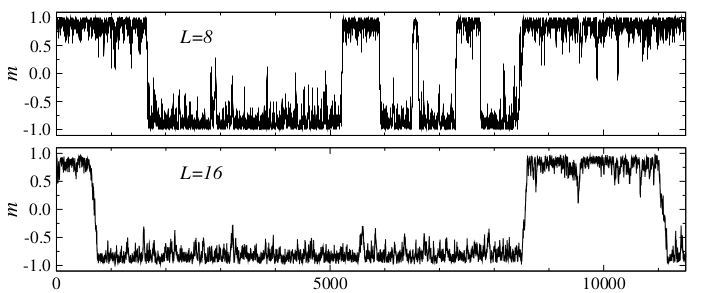
\includegraphics[scale=0.5]{fig11}
\caption{Временные ряды намагниченности, полученные при моделировании Монте-Карло модели Изинга на решетках $L × L$ с $L = 8$ (вверху) и $L = 16$ (внизу) при температуре $T / J = 2.2$ ($<T_c \approx 2.269$). В обоих случаях начальная конфигурация была полностью поляризована, $m = 1$, а последующие точки разделены $N = L^2$ попытками переворота спина в Метрополисе (составляющих одну развертку Монте-Карло).}
\label{}
\end{figure}

Здесь можно увидеть, что намагниченность колеблется между положительными и отрицательными значениями, и что типичное время, необходимое для изменения знака $m$, больше для большей системы. Построение ряда за более длительный период времени делает это более ясным, но нужно обратить внимание, что время, которое система тратит близко к $m = 0$, заметно меньше для $L = 16$, чем для $L = 8$, и это, напрямую связано с обычно более длительным временем обращения. Из таких результатов ясно, что распределение значений m достигает максимума при ненулевых положительных и отрицательных значениях для $T<T_c$. При $T> T_c$ распределение представляет собой единственный пик с центром при $m = 0$. Примеры таких распределений показаны на рис. 12.

\begin{figure}[htp]
\centering
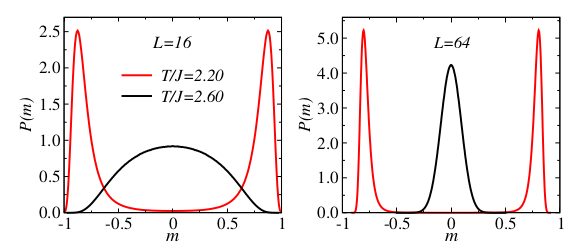
\includegraphics[scale=0.5]{fig12}
\caption{Распределения намагниченности для $L × L$ моделей Изинга с $L = 16$ (слева) и 64 (справа) при двух температурах ниже ($T / J = 2,2$) и выше ($T / J = 2,6$) критической температуры $T_c / J \approx 2,2$}
\label{}
\end{figure}

На языке термодинамики эти два качественно различных распределения можно понимать как следствие свободной энергии $F( m) = E (m) - TS (m)$ при низких $T$ доминирует внутренняя энергия $E$ (которая мала в конфигурациях с большим $| m |$), а при высоких $T$ - энтропия $S$ (которая велика для малых $|m|$).

Двухпиковое распределение намагниченности при низкой температуре предполагает, что даже конечную систему можно рассматривать как упорядоченную, хотя симметрия спиновой инверсии не нарушается при моделировании. Представляется весьма правдоподобным, что типичное время разворота должно отличаться от $L$ (и нетрудно проверить это с помощью данных моделирования для нескольких значений L и подходящего определения разворота), и тогда реверсирование не произойдет для больших $L$, даже во время очень долгих симуляций. Причина этого расходящегося временного масштаба заключается в том, что для того, чтобы намагниченность изменилась, серия локальных переворотов спина обязательно должна провести систему через множество конфигураций с $m \approx 0$, которые имеют все более высокую энергию для увеличения размера системы (и, следовательно, , нижняя больцмановская вероятность). Поэтому для большой системы распределение для $T <T_c$ выбирается только среди подмножества конфигураций с фиксированным знаком $m$ - случайный процесс на практике становится неэргодическим. Нарушенная симметрия и неэргодическая выборка проявляются строго только при $N = ∞$, но на практике также для больших, но конечных систем на временных масштабах, меньших типичного времени перемагничивания. Этот временной масштаб, конечно, зависит от деталей того, как спиновые конфигурации подвергаются термической выборке - в моделировании Монте-Карло и в реальных магнитах, - но расходится при $N → ∞$ для любой схемы локальной выборки.

Обычно при моделировании Монте-Карло не исследуются временные ряды и полное распределение физических величин (хотя иногда это полезно). Вычисляя $\langle m^2 \rangle$ или $\langle |m| \rangle$, нам не нужно беспокоиться о временном масштабе разворотов.
Обычно мы хотим экстраполировать результаты с конечным числом $N$ до термодинамического предела, где $|\langle m \rangle | = \langle |m| \rangle = \langle m^2 \rangle^{1/2}$ (но обратите внимание, что $\langle m^2 \rangle ^{1/2} \ne \langle |m| \rangle$ для конечного N из-за конечной ширины пиков в $m$-распределении).

~\emph{Автокорреляции и статистические ошибки.}

Прежде чем рассчитывать математические ожидания, мы должны обсудить, как статистически анализировать данные Монте-Карло. Последовательные конфигурации, созданные с помощью алгоритма Metropolis, не являются статистически независимыми - статистически независимыми являются только конфигурации, разделенные числом разверток, намного превышающим время автокорреляции. Автокорреляционная функция для величины $Q$ определяется как

\begin{equation}
A_Q(t)=\frac{\langle Q(i+t)Q(i)\rangle - \langle Q\rangle ^2}{\langle Q^2\rangle- \langle Q\rangle^2}
\label{eq_46}
\end{equation}

где $t$ и $i$ обозначают время моделирования, обычно в единицах разверток Монте-Карло, определенных выше, а средние значения относятся к контрольному времени $i$. Нормализация такова, что $A_Q(0) = 1$ и $A_Q(t → ∞) = 0$. Асимптотический спад является экспоненциальным, $A_Q(t) \sim e^{−t/\tau_Q}$, который можно использовать для определения времени автокорреляции $\tau$. Обычно вместо этого используется интегрированное время автокорреляции, которое также содержит вклады от часто доминирующего неасимптотического поведения;

\begin{equation}
\tau_Q^{int}=\frac{1}{2}+\sum\limits_{t=1}^{∞}A_Q(t)
\label{eq_47}
\end{equation}

Здесь мы не будем подробно обсуждать автокорреляции, а только суммируем их основную роль в определении статистической точности (<<планки ошибок>>) вычисленных величин.

Время автокорреляции для $m$ модели Изинга примерно соответствует типичному времени между перемагничиваниями (как на рис. 11). Другие величины, такие как $m^2$ и $| m |$, которые не чувствительны к знаку $m$, имеют более короткое время автокорреляции (однако часто намного дольше, чем один анализ Монте-Карло). Длительное время автокорреляции не влияет на вычисленное среднее значение (т.е. правильно измерять $Q$ после каждой развертки Монте-Карло, даже если $\tau_Q >> 1$), при условии, что общее время моделирования намного больше, чем $\tau_Q$.
Однако время автокорреляции играет важную роль (явно или неявно) при вычислении статистических ошибок.

Чтобы вычислить статистические ошибки, можно разделить моделирование на количество B интервалов, каждый из которых содержит некоторое количество M разверток Монте-Карло. Для некоторой величины $Q$ в среднем $\overline{Q}_b, b = 1,\dots, B$ вычисляются для каждого интервала, а окончательное среднее значение $\overline{Q}$ и шкала ошибок $\sigma_Q$ (одно стандартное отклонение среднего значений интервалов) вычисляются в соответствии с

\begin{equation}
\overline{Q} = \frac{1}{B}\sum\limits_{b=1}{B}\overline{Q}_b
\label{eq_48}
\end{equation}

\begin{equation*}
{\sigma}_Q^2=\frac{1}{B(B-1)}\sum\limits_{b=1}^B (\overline{Q}_b - \overline{Q})^2
\end{equation*}

Окончательная оценка истинного математического ожидания $\langle Q \rangle$ тогда должна быть указана как $\overline{Q} \pm \sigma_Q$

Причина разделения данных заключается в том, что согласно центральной предельной теореме распределение средних значений бина является гауссовым для больших $M$ (в отличие от распределения отдельных измерений, как ясно видно для намагниченности на рис.12), а вычисленная ошибка bar тогда имеет четко определенное уникальное значение (например, мы знаем, что вероятность $\langle Q \rangle$ нахождение в пределах одной полосы погрешности от $Q$ составляет около $2/3$). Это верно только в том случае, если длина ячейки M также намного больше, чем время автокорреляции, так что средние значения ячейки можно рассматривать как статистически независимые. Если это так , шкала погрешности должна зависеть только от общего количества проходов; $\sigma_Q \sim \frac{1}{\sqrt{MB}}$, где коэффициент пропорциональности $\sim \sqrt{\tau_Q}$ (и, конечно, также зависит от подробной формы распределения отдельных измеренных значений $Q$). Нет необходимости вычислять $\tau_Q$ явно. Если есть какие-либо сомнения в том, что интервалы достаточно длинные, это можно проверить, используя довольно большое количество интервалов (например, в диапазоне 100-1000) и сохраняя все средние значения интервалов на диске. Затем данные могут быть повторно разбиты на более длинные интервалы после моделирования, и может быть проверена сходимость $\sigma_Q$ как функция длины интервала. 

Важно отметить, что время автокорреляции любой схемы локального обновления, например, алгоритма Метрополиса, расходится при $T → T_c$ и $​​N → ∞$.

Ранее мы видели пример этого во времени перемагничивания модели Изинга, но расходящиеся времена автокорреляции также влияют на любую величину (в частности, $m^2$ и $|m|$), которая чувствительна к флуктуациям величины $m$ (что на практике справедливо для большинства представляющих интерес количеств). Поэтому трудно получить хорошие результаты для больших систем, близких к критической точке. Во многих случаях, включая модель Изинга, эта проблема может быть решена (или почти решена) с помощью кластерных алгоритмов ~\cite{prl_58_86, prl_62_361}, где кластеры спинов (построенные таким образом, чтобы удовлетворить детальный баланс) переворачиваются вместе (вместо того, чтобы переворачивать отдельные вращается одно за другим). Классические кластерные алгоритмы подробно описаны в литературе ~\cite{Landau_Binder, Newman_Barkema} . Обсуждаемые ниже результаты Изинга для систем с числом спинов до $1024^2$ фактически были получены с использованием кластерного алгоритма. Было бы очень сложно сгенерировать (в разумные сроки) данные такого же качества, используя схему Метрополиса для таких больших систем в критическом регионе.

\subsection{Масштабирование конечных размеров и критические показатели}
На рис. 13 (а) показана температурная зависимость квадрата намагниченности $\langle m^2 \rangle$ 2D-модели Изинга для нескольких размеров решетки. Все более резкая особенность проявляется с увеличением $L$ в окрестности известного $T_c$, и кажется весьма вероятным, что $\langle m^2 \rangle$ обращается в нуль при $N → ∞$ при $T> T_c$ и остается ненулевым при $T <T_c$. На этом графике полосы погрешностей не видны, потому что они намного меньше ширины линии. Данные были сгенерированы на очень тонкой Т-образной сетке для получения непрерывных кривых.

\begin{figure}[htp]
\centering
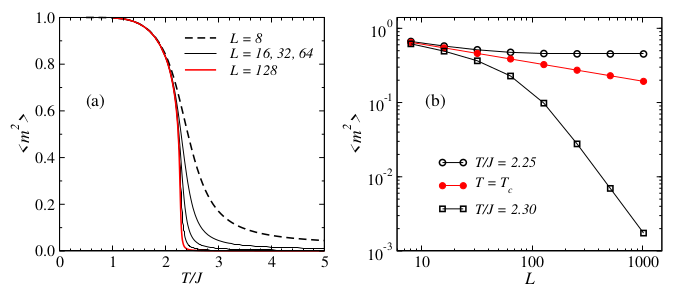
\includegraphics[scale=0.5]{fig13}
\caption{(а) Квадрат намагниченности как функция температуры для нескольких систем Изинга $L × L$.
(б) Зависимость от конечных размеров при $T_c$, ниже и выше. При $T$ c поведение является степенным, $m^2 \sim L^{−1/4}$, что на этой логарифмической шкале соответствует линии с наклоном $-1/4$. При $T> T_c$ убыль к нулю имеет вид $L^{−2}$, и это также скорость сходимости при $T <T_c$.}
\label{}
\end{figure}

Зависимость $\langle m^2 \rangle$ от размера при трех различных температурах показана на рис. 13 (б). Для $T <T_c$ он сходится с $L$ к ненулевому значению, в то время как для $T> T_c$ он уменьшается до $0$ как $L^{-2}$.
Точно при $T_c$ распад происходит по нетривиальному степенному закону; $\langle m^2 \rangle \sim L^{-2\beta/\nu}$, где $\beta = 1/8$ - тот же показатель степени, что и в намагниченности $N = ∞$ для $T <T_c$, а $\nu$ (показатель корреляционной длины, который будет обсуждаться ниже) равен 1 для этой модели. Такое поведение - пример масштабирования конечного размера. Идеальное степенное поведение при критичности соблюдается строго только при $L → ∞$, в то время как для небольших систем могут быть существенные поправки к масштабированию (которые необычно малы в случае обсуждаемой здесь модели Изинга). Обычно мы не знаем точного значения $T_c$ (что, конечно, может быть одной из причин, по которой выполняется моделирование), и тогда необходимо разработать процедуры для определения местоположения критической точки.
Есть много способов сделать это, и все они так или иначе основаны на том факте, что параметр порядка и связанные с ним величины должны вести себя как нетривиальные степенные законы (с известными или неизвестными показателями) для больших решеток в критической точке.

Квадрат намагниченности связан со спиновой корреляционной функцией,

\begin{equation}
C(r_{ij})=\langle \sigma_i \sigma_j\rangle
\label{eq_49}
\end{equation}

где $r_{ij}$ - расстояние между спинами. Если есть дальний порядок, то $C(r) →  \langle m^2 \rangle$ при $r → ∞$ в бесконечной решетке. Для конечных систем то же самое верно для $C(r_max)$ в пределе $L → ∞$, где $r_max$ - наибольшее расстояние на периодической решетке, например, $r_max = \sqrt{2L}$ для
решетки $L × L$. Если порядок отсутствует, то $C(r) → 0$ согласно степенному закону при $T_c$ и экспоненциально при $T> T_c$. Ниже $T_c$ в бесконечной системе «связная» корреляционная функция,

\begin{equation}
C^{*}(r)=C(r)-\langle m \rangle ^2
\label{eq_50}
\end{equation}

экспоненциально убывает до нуля при $r → ∞$. Экспоненциальные формы $C(r)$ и $C^{∗}(r)$ характеризуются корреляционной длиной $\xi$, которая расходится при $T → T_c$ с обеих сторон.

Отметим также, что $\langle m^2 \rangle$ может быть записано в точности как сумма спиновых корреляций;

\begin{equation}
\langle m^2 \rangle = \frac{1}{N}\sum\limits_{r}C(r)
\label{eq_51}
\end{equation}

$L^{−2}$-сходимость $\langle m^2 \rangle$ (как ниже, так и выше $T_c$) просто связана с конечной корреляционной длиной.

Здесь следует указать, что характер спиновых корреляций ниже $T_c$ зависит от симметрии параметра порядка, с которым мы имеем дело. Для векторного параметра порядка, например, в модели Гейзенберга (с классическими или квантовыми спинами), корреляции спиновых компонент, параллельных (продольных) параметру порядка системы с нарушенной симметрией, затухают по экспоненте, как в модели Изинга. Однако поперечные корреляции затухают по степенному закону. Это связано с непрерывной симметрией параметра порядка.

В модели Изинга симметрия дискретна - упорядоченное состояние нарушает симметрию спиновой инверсии, и затраты свободной энергии локальной флуктуации намагниченности велики (пропорциональны границе перевернутого домена). Это приводит к экспоненциально убывающей (связанной) корреляционной функции в упорядоченной фазе. С другой стороны, в модели Гейзенберга существуют бесщелевые спин-волновые возбуждения (которые представляют собой возбуждения спинов в направлениях, поперечных направлению упорядочения и в более общем смысле называемые модами Голдстоуна). Колебания из-за них приводят к степенной форме поперечных спиновых корреляций. Тогда поперечная корреляционная длина формально бесконечна, и в расчетах с конечной решеткой, в которых вращательная симметрия явно не нарушена (так что вычисленное $\langle m_s^2 \rangle$ содержит вклады как продольных, так и поперечных корреляций), размерные поправки к $\langle m_s^2 \rangle$ пропорциональны $ \sim 1/L$. Мы уже обсуждали это поведение в основном состоянии 2D-антиферромагнетика $S = 1/2$ Гейзенберга в гл. 2.4, а на рис. 5 (b) очень четко показаны поправки $1/L$.

\subsubsection{Масштабирование и критические показатели}
Чтобы обсудить масштабирование конечного размера вблизи критической точки более подробно, мы сначала должны рассмотреть некоторые основные аспекты критических явлений в термодинамическом пределе. Мы перечислим здесь только некоторые ключевые результаты и определения ~\cite{cardy} для получения более подробной информации.

Корреляционная длина - одно из важнейших понятий, лежащих в основе теории фазовых переходов и критических явлений. В бесконечной системе по мере приближения к критической температуре корреляционная длина расходится по степенному закону;

\begin{equation}
\xi \sim |t|^{-\nu}
\label{eq_52}
\end{equation}

Показатель $\nu$ остается таким же при приближении к $T_c$ сверху или снизу, но префактор в (52) в целом различен для $t → 0^{+}$ и $t → 0^{-}$ (однако отношения этих предварительных факторов, называемые отношениями амплитуд, часто универсальный). В рамках теории среднего поля $\nu = 1/2$. Именно при $T_c$, хотя корреляционная длина формально бесконечна, система еще не упорядочена. Вместо этого для бесконечной системы корреляционная функция точно при $T_c$ имеет степенной вид:

\begin{equation}
C(r) \sim r^{-(d-2+\eta)}
\label{eq_53}
\end{equation}

где d - размерность системы, а $\eta$ - еще один критический показатель (также называемый аномальной размерностью, потому что он может быть связан с фрактальной размерностью упорядоченных областей в критической точке), среднее значение которого равно $\eta = 0$ Дальний порядок устанавливается лишь бесконечно ниже $T_c$, где асимптотическая корреляция на больших расстояниях приближается к константе; $C(r → ∞) = \langle m^2 \rangle$.

Мы уже обсуждали поведение параметра порядка в состоянии с нарушенной симметрией при $t → 0^{-}$;

\begin{equation}
\langle m \rangle \sim |t|^\beta
\label{eq_54}
\end{equation}

Нас также будет интересовать соответствующая восприимчивость, определяемая как

\begin{equation}
\xi = \frac{d\langle m \rangle}{dh}|_{h→0} = \frac{N}{T}(\langle m \rangle^2 - \langle m \rangle^2)
\label{eq_55}
\end{equation}

где $h$ - сила связи поля с параметром порядка, например, в случае ферромагнетика Изинга член гамильтониана $−h\sum \sigma_i$. Последнее выражение в (~\ref{eq_55}) явно показывает, как $\xi$ напрямую связано с флуктуациями параметра порядка. Восприимчивость расходится при $T_c$;

\begin{equation}
\xi = \frac{d\langle m \rangle}{dh}|_{h→0} = \frac{N}{T}(\langle m \rangle^2 - \langle m \rangle^2)
\label{eq_56}
\end{equation}

Таким образом, при приближении к критической точке система становится бесконечно чувствительной к полю $h$, взаимодействующему с параметром порядка, и именно при $T_c$ форма линейного отклика $\langle m \rangle = \xi h$ перестает действовать. Вместо этого при $T_c$ параметр порядка зависит от (слабого) поля как $h^{1/ \delta}$.
Согласно результату в формуле (~\ref{39}) среднеполевое значение показателя $\delta = 3$.

Удельная теплоемкость также сингулярна при $T_c$,

\begin{equation}
C \sim |t|^{-\alpha}
\label{eq_57}
\end{equation}

где $\alpha$ может быть положительным или отрицательным. В теории среднего поля $\alpha=0$. Когда $\alpha<0$, расходимости нет, только особенность возврата в точке $T_c$. В некоторых случаях, например, для 2D-модели Изинга, $\alpha=0$, но все еще сохраняется слабая логарифмическая дивергенция теплоемкости.

Критические показатели $\nu,\beta,\eta$ и т. д., c которыми мы столкнулись выше, не все независимы друг от друга. Связь между показателями объясняется теорией ренормализационной группы, которая для обсуждаемого здесь типа переходов порядок-беспорядок показывает, что есть еще два фундаментальных показателя, в терминах которых можно записать физически наблюдаемые показатели ~\cite{cardy}. Экспонентные отношения были найдены с использованием других аргументов еще до появления этой окончательной теории фазовых переходов (в наиболее полной форме Уидом в середине 1960-х годов), например,

\begin{equation*}
\gamma = \nu(2-\eta)
\end{equation*}

\begin{equation}
\nu d = 2 - \alpha
\label{eq_58}
\end{equation}

\begin{equation*}
\alpha + 2\beta + \gamma = 2
\end{equation*}

Такие соотношения очень полезны для проверки непротиворечивости численных расчетов показателей. Отношения экспонент, включающие размерность d, называются отношениями гипермасштабирования и являются менее общими, чем другие отношения. Они не применимы, например, в рамках теории среднего поля и, следовательно, для любой системы с верхним критическим размером или выше.

\subsubsection{Гипотеза конечного масштабирования}
Основное предположение, лежащее в основе теории масштабирования конечных размеров ~\cite{prl_28_1516}, состоит в том, что отклонения от критического поведения бесконечного размера должны происходить, когда корреляционная длина $\xi$ (бесконечной системы) становится сравнимой с длиной конечной системы $L$. Если$ L >>\xi$, Тот факт, что система конечна, не должен иметь значения, и применимо поведение бесконечного размера.
С другой стороны, если $L<<\xi$, то $L$, а не $\xi$, должен быть наиболее подходящим масштабом длины. Чтобы увидеть, как две шкалы длины вступают в игру, полезно выразить интересующие количества в терминах длины корреляции. Рассмотрим величину $Q$, которая демонстрирует степенное расходящееся поведение при $T_c$ (приведенная температура $t → 0$),

\begin{equation}
Q \sim |t|^{-k}
\label{eq_59}
\end{equation}

например, восприимчивость (в этом случае $k = \gamma$). Мы можем использовать уравнение (~\ref{eq_52}) выразить $| t |$ как функция корреляционной длины;

\begin{equation}
Q \sim \xi^{-1/\nu }
\label{eq_60}
\end{equation}

и используя это, мы можем записать $Q$ как

\begin{equation}
Q \sim \xi^{k/\nu }
\label{eq_61}
\end{equation}

Эта форма должна применяться для $\xi << L$, но когда $\xi \sim L$ расходимость больше не может продолжаться на конечной решетке. Максимальное значение $Q_max$, достижимое $Q$ на конечной решетке, тогда должно быть получено заменой $\xi → L$ в уравнении (~\ref{eq_61}), давая

\begin{equation}
Q_{max}(L) \sim L^{k/\nu }
\label{eq_62}
\end{equation}

Таким же образом из уравнения (~\ref{eq_60}) мы также можем вывести масштаб приведенной температуры, при которой $\xi$ достигает $L$, которая также должна быть температурой, при которой достигается максимальное значение величины $Q$;

\begin{equation}
|t_{max}(L)| \sim L^{-1/\nu }
\label{eq_63}
\end{equation}

Следует отметить, что это просто пропорциональность, и число перед $L^{−1 / \nu }$ зависит от количества. Сдвиг также применяется к недивергентным величинам - любая особенность, которая проявляет сингулярное поведение при $T → T_c$, должна сдвигаться со скоростью $L^{−1 / \nu }$. Если есть четко определенный максимум или другая различимая особенность в некоторой величине при $T = T^{∗} (L)$, то эту температуру можно использовать как критическую температуру, зависящую от размера (и, опять же, эта температура не уникальна, но зависит от количество считается).

Законы масштабирования конечного размера (~\ref{eq_62}) и (~\ref{eq_63}) следуют из более общей гипотезы масштабирования конечного размера ~\cite{prl_28_1516}, которая, как и теория масштабирования для бесконечных систем, первоначально была предложена на основе феноменологических соображений, но позже была получена с использованием теория ренормгруппы. Гипотеза состоит в том, что наблюдаемая, сингулярная при $T_c$ в термодинамическом пределе, масштабируется с размером системы, близким к $T_c$, как степень $L$, умноженная на невырожденную функцию отношения $\xi / L$. Таким образом, любая сингулярная величина (не обязательно расходящаяся) должна иметь вид

\begin{equation}
Q(t,L) = L^\sigma f(\xi/L)
\label{eq_64}
\end{equation}

который, используя $\xi \sim | t |^{ −1 / \nu }$, мы также можем записать как

\begin{equation}
Q(t,L) = L^\sigma g(tL^{1/\nu })
\label{eq_65}
\end{equation}

Этот закон масштабирования должен выполняться как выше $(t> 0)$, так и ниже $(t <0)$ критической точки. Точно при $T_c$ мы восстанавливаем масштабирование $Q(0, L) \sim L^\sigma$. Чтобы связать $\sigma$ со стандартными критическими показателями, мы можем использовать тот факт, что при фиксированном $t$, близком к 0, по мере роста системы поведение для любого $t \ne 0$ в конечном итоге должно быть задано уравнением (~\ref{eq_59}); $Q (t, L → ∞) \sim | t |^{-k}$ (где $k$ отрицательно для сингулярной недивергентной величины, например, для параметра порядка мы имеем $k = -\beta $). Чтобы получить эту форму, масштабирующая функция $g (x)$ в (65) должна асимптотически вести себя как $g(x) \sim x^{-k}$ при $x → ∞$. Таким образом, чтобы размерная зависимость в (~\ref{65}) сокращалась, мы заключаем, что $\sigma = k / \nu $, т.е.

\begin{equation}
Q(t,L) = L^{k/ \nu }g(tL^{1/\nu })
\label{eq_66}
\end{equation}

Чтобы извлечь масштабирующую функцию $g(x)$ с использованием числовых данных, можно определить

\begin{equation}
y_L = Q(t,L)L^{-k/\nu}, x_L=tL^{1/\nu }
\label{eq_66}
\end{equation}

и построить график зависимости $y_L$ от $x_L$ для систем разных размеров. Если гипотеза масштабирования верна, данные для разных (больших) систем должны попадать на одну и ту же кривую, которая в таком случае является функцией масштабирования (это называется схлопыванием кривых друг на друга); $g(x) = y_{ L → ∞}(x)$. Рис. 14 иллюстрирует это с использованием данных Монте-Карло для магнитной восприимчивости 2D-модели Изинга. Местоположение пика на панели (a) явно смещается в сторону известного T c с увеличением L. После масштабирования данных в соответствии с вышеуказанными процедурами, как показано на панели (b), кривые действительно сжимаются почти друг на друга близко к $t = 0$, но дальше от критической точки наблюдаются отклонения для меньших систем. Это связано с поправками к масштабированию, которые в принципе можно описать с помощью вспомогательных показателей.

\begin{figure}[htp]
\centering
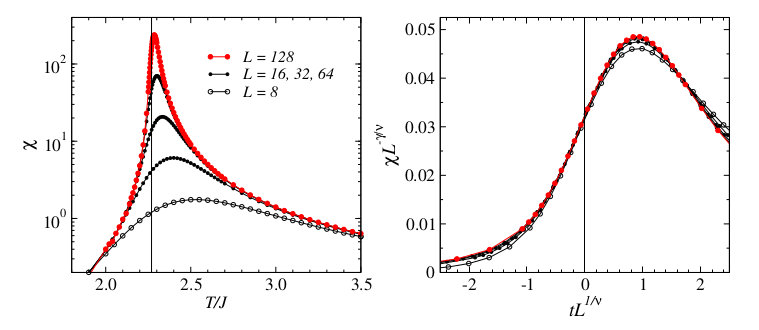
\includegraphics[scale=0.5]{fig14}
\caption{Результаты Монте-Карло для восприимчивости (55) модели Изинга на нескольких различных решетках $L × L$. (a) показывает температурную зависимость, вертикальная линия указывает $T_c$. Обратите внимание на вертикальный масштаб журнала. В (b) данные были масштабированы с использованием точных значений показателей Изинга, $\gamma = 7/4$ и $\nu = 1$, и точного значения $T_c$ в $t = (T - T_c) / T_c$}
\label{}
\end{figure}

Мы можем применить масштабную форму (~\ref{eq_66}) к самой длине корреляции, для которой $k = \nu $ и $L$-масштабирование не зависит от конкретных показателей модели. В случаях, когда класс универсальности неизвестен априори, это полезно для извлечения показателя $\nu$ по кривым - коллапсирования данных $\xi/L$ без одновременной корректировки другого показателя $k$ в (~\ref{eq_66}).\\

~\emph{Практические определения длины корреляции.}

Длина корреляции может быть определена различными способами, не обязательно только на основе асимптотического убывания корреляционной функции (которую часто трудно надежно извлечь). Одно практическое и обычно используемое определение длины корреляции основано на преобразовании Фурье корреляционной функции, часто называемом (статическим) структурным фактором,

\begin{equation}
S(q) = \langle \sigma_{-q}\sigma_q\rangle = \sum\limits_{r}e^{-iqr}C(r)=\sum\limits_{r}cos(qr)C(r)
\label{eq_68}
\end{equation}

где $\sigma_q$ - преобразование Фурье отдельной спиновой конфигурации,
\begin{equation}
\sigma_q = \frac{1}{\sqrt{N}}\sum\limits_{j} \sigma_j e^{-iqr_j}
\label{eq_69}
\end{equation}

Обозначим через Q волновой вектор доминирующих корреляций - для ферромагнетика $Q = 0$, для 2D-антиферромагнетика $Q = (\pi, \pi)$ и т. Д. Для упрощения обозначений $q$ будет использоваться для отклонения от $Q$. Тогда $q_1 = 2\pi / L$ соответствует одному из волновых векторов, ближайших к $Q$, например, $Q + (2 \pi / L) \hat{x}$, где $\hat{x}$ - единичный вектор обратного пространства в $x$-направлении.

Корреляционная длина $\xi$ a может быть определена с использованием структурных факторов при $q = 0$ и $q_1$;

где $\sigma_q$ - преобразование Фурье отдельной спиновой конфигурации,
\begin{equation}
\xi_a=\frac{1}{q_1}\sqrt{\frac{S(0)}{S(q_1)}-1}
\label{eq_70}
\end{equation}

Можно показать, что для $d$-мерной решетки, если корреляционная функция задается формой Орнштейна-Цернике (полученной при рассмотрении среднего поля ~\cite{cardy}),

\begin{equation}
C_{OZ}(r) \sim r^{-\frac{1}{2}(d-2)}e^{-r/\xi}
\label{eq_71}
\end{equation}

тогда $\xi_a$ связано с исходной корреляционной длиной $\xi$, появляющейся в экспоненциальном убывании этой корреляционной функции согласно

\begin{equation}
\xi_a=\xi \sqrt{\frac{(1+d)(3+d)}{8d}}
\label{eq_72}
\end{equation}

Таким образом, для $d = 1$ и 3 $\xi_a = \xi$, в то время как двумерный случай является частным, с $\xi_a = \xi(15/16)^{1/2}$ (или, можно сказать, что $d = 1,3$ являются частными случаями, поскольку множитель отличается от единицы также при всех $d> 3$). Форма Орнштейна-Цернике обычно справедлива в неупорядоченных 
фазах при $r>>\xi$ ~\cite{cardy}. Отклонения от этой формы на малых расстояниях означают, что (~\ref{eq_72}) не выполняется в точности, но независимо от поведения на малых расстояниях это соотношение выполняется именно тогда, когда $\xi → ∞ $.

В случае дальнодействующей классической системы $\xi_a$ обычно расходится при $T → 0$ для любого $L$, поскольку в основном состоянии нет флуктуаций (и, таким образом, структурный фактор обращается в нуль при $q \ne 0$. Чтобы удалить вклады от неубывающей части корреляционной функции в упорядоченной системе, мы можем использовать связанную корреляционную функцию (~\ref{eq_50}). Хотя $\langle m \rangle ^2$ не определен однозначно для конечной системы, можно, например, вычесть $C(r_{max})$. В качестве альтернативы мы можем использовать другое определение длины корреляции, основанное на структурном факторе при $q_1$ и $q_2 = 2q_1 = 4 \pi / L$;

\begin{equation}
\xi_b=\frac{1}{q_1} \sqrt{\frac{S(q_1/S(q_2)-1)}{4-S(q_1)/S(q_2)}}
\label{eq_73}
\end{equation}

Можно показать, что (~\ref{eq_72}) также выполняется для этого определения, если $C(r)$ задается корреляционной функцией Орнштейна-Цернике, а также когда добавляется константа, соответствующая дальнему порядку, для $T <T_c$ (поскольку это влияет только на $S(0)$ ).

На рис. 15 показаны результаты для $\xi_a/L$ и $\xi_b/L$ для 2D-модели Изинга. Обратите внимание, что в случае расходящейся $\xi_a/L$ при $T → 0$ используется логарифмический масштаб, в то время как $\xi_b/L$ сходится и отображается в линейном масштабе. Обе величины демонстрируют независимость от размера (кривые пересекают друг друга) при $T_c$, но их значения явно различаются. 

\begin{figure}[htp]
\centering
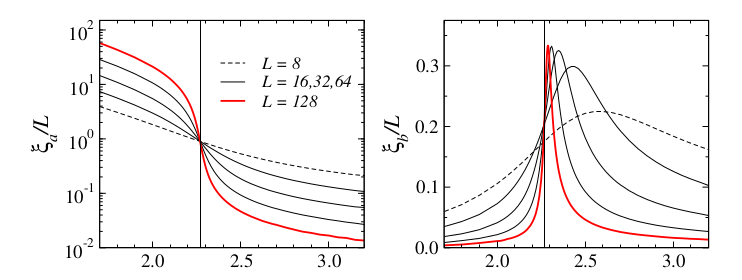
\includegraphics[scale=0.5]{fig15}
\caption{Температурная зависимость двух определений корреляционной длины, уравнения (~\ref{eq_70}) и (~\ref{eq_73}), нормированные на размер $L$ для моделей Изинга $L × L$. Вертикальные линии обозначают $T_c$}
\label{}
\end{figure}

Это связано с тем, что форма корреляционной функции Орнштейна-Цернике применяется асимптотически только для $T> T_c$, и нет причин, по которым два определения $\xi_a$ и $\xi_b$ должны точно совпадать при $T_c$ (хотя их значения должны быть связаны). Их значения очень близки для больших систем, близких к $T_c$ в неупорядоченной фазе. Точки пересечения (или положение пика $\xi_b$) можно использовать для извлечения $T_c$ в системах, где оно неизвестно. Ось температуры также можно масштабировать таким же образом, как на рис. 14, для извлечения показателя корреляционной длины.

Обратите внимание, что для небольшого количества необходимых $q$-точек $S(q)$ может быть эффективно вычислено с использованием преобразования Фурье (~\ref{eq_69}) спиновых конфигураций, созданных при моделировании Монте-Карло. Поскольку структурный фактор действительный, имеем

\begin{equation}
S(q)=\langle Re(\sigma_q)^2 \rangle + \langle Im(\sigma_q )^2 \rangle
\label{eq_74}
\end{equation}

Вычисление полной корреляционной функции $C(r)$ и ее преобразование Фурье после моделирования занимает гораздо больше времени.

~\emph{Соотношение связующего и кумулянта}

Помимо $\xi / L$, существуют также другие безразмерные величины, которые не зависят от размера в критической точке и полезны для извлечения $T_c$ независимо от значений критического показателя. Пожалуй, наиболее часто используемым является соотношение Биндера ~\cite{prl_47_693, prb_30_1477}:

\begin{equation}
R_2 = \frac{\langle m^4 \rangle}{\langle m^2\rangle ^2}
\label{eq_75}
\end{equation}

При $T_c$ степенные законы сокращаются, и отношение не зависит от $L$ (а также универсально), вплоть до дополнительных поправок конечного размера. Обычно построение графика зависимости $R$ от $T$ для систем разных размеров дает кривые, которые пересекаются друг с другом близко к $T_c$. Обнаруживая точки, в которых $R_2$ для пар размеров системы (например, $L$ и $2L$) пересекают друг друга, можно получить критическую точку, зависящую от размера, которая обычно сходится быстрее, чем сдвиг $L^{ −1/\nu}$ в (~\ref{eq_63}). Можно думать об этом как о результате отмены основных поправок в количестве, включающем два размера системы, а затем остается что-то, что приближается к $T_c$ в соответствии с более быстрой коррекцией масштабирования более высокого порядка. Можно также определить отношения, аналогичные (~\ref{eq_75}), на основе других степеней $m$, например, $R_1 = \frac{\langle m^2 \rangle}{\langle |m| \rangle} $. Метод пересечения кривой для определения местоположения $T_c$ также может применяться таким же образом с $\xi/L$.

Соотношение связующего также имеет другие интересные свойства. В случае скалярного параметра порядка (например, для модели Изинга) кумулянт Биндера определяется как

\begin{equation}
U_2 = \frac{3}{2}(1-\frac{1}{3}R_2)
\label{eq_76}
\end{equation}

В упорядоченном состоянии $U_2 → 1$ при $N \to \infty$, поскольку распределение намагниченности $P(m)$ тогда приближается к двум дельта-функциям при $\pm \langle |m| \rangle $, и, следовательно, $R_2 \to 1$. Напротив, в неупорядоченной фазе флуктуации $m$ гауссовы около $m = 0$ (что следует из центральной предельной теоремы, поскольку флуктуации в областях, разделенных расстоянием $>>\xi$ в большой системе, некоррелированы). На основе гауссовых интегралов $R_2 \to 3$ и $U_2 \to 0$.
Обобщая кумулянт Биндера до n-компонентного параметра порядка (где $n = 1$ для намагниченности Изинга, $n = 2$ для модели $XY$ и т. д.), Следует иметь в виду, что $m^2 = m · m$ и $m^4$ в ( ~\ref{eq_75}) нечувствительны к угловым флуктуациям параметра порядка. Интегрируя гауссово распределение $|m|$ в n-мерном пространстве для вычисления средних значений в ( ~\ref{eq_75}), однако, вводит n-зависимые факторы. Чтобы воспроизвести указанные выше свойства $U_2$, необходимо определить его для общего параметра порядка как

\begin{equation}
U_2 = \frac{n+2}{2}(1-\frac{n}{ n+2 } R_2)
\label{eq_77}
\end{equation}

На рис. 16 показаны результаты Монте-Карло для $U_2$ как функции $T$ для нескольких двумерных решеток. Ясно видно развитие ступенчатой функции при $T_c$ с увеличением размера системы. В этом случае все кривые пересекают друг друга очень близко к известной $T_c$, отражая очень маленькие дополнительные исправления в этой модели. В других системах обычно наблюдается некоторый дрейф пересечений, и необходимо проводить тщательную экстраполяцию точек пересечения (например, на основе наборов данных для размеров $L$ и $2L$ или некоторых других соотношений сторон).

\begin{figure}[htp]
\centering
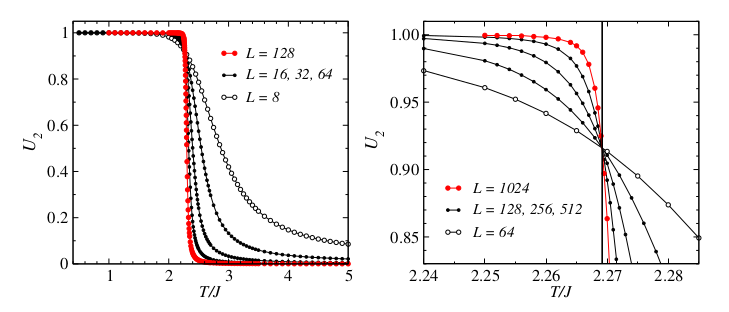
\includegraphics[scale=0.5]{fig16}
\caption{Кумулянт Биндера (76) для моделей Изинга $L × L$. На (а) можно увидеть приближение к предельным значениям $U_2 → 0$ (для $T> T_c$) и $U_2 → 1$ (для $T <T_c$) для увеличения $L$. На (b) данные, близкие к $T_c$ (вертикальная линия) нанесены на график в более подробном масштабе, а для большего $L$ показано пересечение кривых.}
\label{}
\end{figure}

~\emph{Конечное масштабирование на практике}

Мы кратко обсудим, как выполнить коллапс данных конечного размера на практике. Количество задействованных параметров (то есть $T_c$, а также один или два показателя степени и, возможно, также показатели степени вспомогательных поправок, которые будут обсуждаться ниже) довольно мало, и обычно можно получить некоторое приблизительное представление об их значениях, просто взглянув на необработанные данные. и выполнение некоторых начальных экспериментов, например, просто обнаружив нетривиальное степенное поведение, как на рис. 13 [и этого часто может быть достаточно для определения отношения экспонент $k / \nu$ в уравнениях. (~\ref{eq_62}) и (~\ref{eq_66}). Анализ кумулянта Биндера или $\xi / L$, возможно, уже дал $T$ c с достаточной точностью, но все же может быть полезно проверить чувствительность других соответствует его значению. Благодаря мощности современных компьютеров в качестве альтернативы использованию сложной процедуры многомерной оптимизации можно написать простую компьютерную программу методом грубой силы для поиска наилучшего набора параметров на подходящей конечной сетке. Качество коллапса данных, производимого набором параметров, может быть количественно определено как значение $\xi^2$, полученное путем подбора одного полинома высокого порядка через все масштабированные точки данных $(x_L, y_L)$, определенные в (~\ref{eq_67}), одновременно для всех $L$, по которым имеются данные. Обычно существует большое количество точек данных для разных связей и размеров системы, и, поскольку функция масштабирования должна работать правильно, полином разумного порядка (3-8-й, как приблизительный ориентир) должен хорошо работать в окне, где данные можно свернуть. Размер этого окна также необходимо отрегулировать до тех пор, пока данные не исчезнут. Например, для данных на рис.14, $x$ в диапазоне $(-0,5, 0,5)$ должен быть подходящим, хотя окно также зависит от размеров системы, включенных в анализ, и планок погрешностей (которые определяют чувствительность к пренебрегли поправками к субсидированию масштабирования).

Не всегда легко определить надежные планки погрешностей для параметров, полученных при такой подгонке. Помимо чисто статистических ошибок (которые могут быть определены, например, повторением минимизации $\xi^2$ несколько раз с гауссовым шумом, величина которого равна полосе погрешностей, добавленных к данным), существуют также систематические ошибки из-за поправок на масштабирование, которые может быть трудно оценить. Если $\xi^2$ является статистически обоснованным (т.е. близким к 1 на степень свободы), обычно можно предположить, что пренебрегаемые поправки не повлияли на параметры за пределами статистических неопределенностей.

На рис. 17 показан пример коллапса данных. Критические показатели и $T_c$ двухмерной модели Изинга были определены с использованием данных для $L \in {64 - 512}$ в окне $|t| L 1 / \nu <0,5$ (где t содержит переменную $T_c$, скорректированную в процедуре). 

\begin{figure}[htp]
\centering
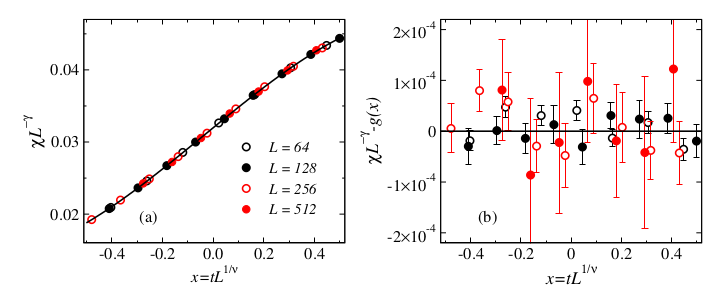
\includegraphics[scale=0.5]{fig17}
\caption{(а) Масштабируемый коллапс восприимчивости 2D-модели Изинга; те же данные, что и на рис.14, но с учетом более крупных решеток и корректировки $T_c$ в $t = (T - T_c) / T_c$, а также показателей $\nu, \gamma$ для минимизации $\xi^2$ относительно масштабирующей функции $g(x)$ в виде полинома (здесь четвертого порядка, показанного сплошной кривой). Оптимальные значения для этого набора данных: $T_c/ J = 2,26921 \pm 0,00002$, $\nu = 0,9985 \pm 0,0011$ и $\gamma = 1,750 \pm 0,002$, где планки ошибок (одно стандартное отклонение) были вычислены путем повторения подгонки несколько раз с помощью гауссова шум (величиной, равной планкам погрешностей Монте-Карло), добавленный к данным. (b) показывает данные с вычтенной функцией подобранного масштабирования $g(x)$, так что полосы ошибок становятся видимыми. Подгонка статистически правильная, с $\xi^2 \approx 0,9$ (на степень свободы).}
\label{}
\end{figure}

Результаты, перечисленные в подписи к рисунку, отлично согласуются с известными показателями $T_c$ и 2D Изинга, а также статистически очень хорошо. Используя то же окно подгонки, нельзя получить статистически приемлемую подгонку, если включены решетки гораздо меньшего размера, например, включение $L = 32$ дает $\xi^2 \approx 2$ (на степень свободы), что незначительно слишком велико для числа степеней свободы соответствия. В этом случае $T_c = 2,26924 \pm 0,00002$, что примерно на 3 планки ошибок выше истинного значения, в то время как показатель степени верен с точностью до двух планок ошибок.

~\emph{Исправления к масштабированию}

В качестве проверки часто бывает хорошей идеей внести некоторые исправления в ведущие формы масштабирования, а иногда даже необходимо сделать это, чтобы получить хорошее соответствие. Наиболее часто используемый метод - свернуть данные с помощью

\begin{equation}
y_L=Q(t,L)L^{-k/\nu}(1+aL^{-\omega})^{-1}
\label{eq_78}
\end{equation}

\begin{equation*}
x_L=tL^{1/\nu}
\end{equation*}

где $\omega$ - старший показатель степени, а $a$ - постоянная. Здесь нет поправки к масштабированию $x_L$ (смещение критической точки на конечные размеры), но такая поправка, в принципе, также может быть включена ~\cite{prb_73_014431} . Обычно хорошее совпадение с поправками может быть получено также при включении размеров решетки, которые необходимо исключить, если поправки не используются.
Более широкий диапазон размеров системы может частично компенсировать тот факт, что статистические неопределенности всех параметров увеличиваются при включении большего количества параметров. Если согласованные ведущие критические показатели получены в подгонках как с поправками, так и без них, то можно быть достаточно уверенным, что результаты верны.

\subsection{Переходы первого рода}
Свойства масштабирования, которые мы обсуждали в предыдущем разделе, применимы к непрерывным фазовым переходам, где корреляционная длина расходится. При переходах первого рода (разрывных) корреляционная длина остается конечной в точке перехода, а параметр порядка, как и другие величины, демонстрирует скачкообразные скачки. Разрывы развиваются в пределе бесконечного размера системы, обычно в соответствии с степенными законами, которые также можно изучать с помощью методов масштабирования конечного размера. Показатели, связанные с этими степенными законами, обычно тривиально связаны с размерностью системы ~\cite{prb_26_2507, phys_91_113, prb_43_3265} [123, 124, 125]. Например, теплоемкость расходится с размером системы как $L^d$ при переходе первого рода, вместо $L^{\alpha/\nu}$, с обычно очень малым (или даже отрицательным) $\alpha$ при непрерывном переходе. Сдвиг критической точки с размером системы масштабируется как $L^{−d}$ вместо смещения $L^{−1/\nu}$ непрерывной критической точки.

Хотя масштабирование конечного размера с показателями, равными d, в принципе, позволяет легко распознать переход первого рода, исследования слабых переходов первого рода затруднены, поскольку они показывают большие поправки к ведущим формам масштабирования. В таком случае может оказаться трудным, учитывая размеры системы, доступные на практике, четко отличить медленно развивающиеся разрывы от более слабого сингулярного поведения при непрерывном переходе.

Переходы сильно первого рода также трудно изучать по совершенно другой причине. Моделирование Монте-Карло может застрять в метастабильном состоянии, и в этом случае вычисленные величины не соответствуют правильным средним тепловым значениям (что, с другой стороны, полностью аналогичен реальным системам, для которых эффекты метастабильности и гистерезиса являются отличительными чертами переходов первого рода). Тогда может быть даже трудно точно определить точку перехода. Чтобы облегчить такие проблемы, были разработаны различные многоканонические методы Монте-Карло, в которых конфигурации отбираются в расширенном ансамбле, где температура системы также колеблется (методы отпуска или параллельного отпуска ~\cite{Marinari, psj_65_1604} [126, 127]), или с помощью распределение, отличное от вероятности Больцмана ~\cite{prl_68_9, pre_86_2050, pre_64_056101, pre_70_046701} (к которому измерения повторно взвешены), что облегчает системе исследование конфигурационного пространства.

\subsubsection{Сосуществование фаз}
Одна из важнейших характеристик перехода первого рода - сосуществование фаз. В моделировании Монте-Карло в точке перехода (на практике в небольшом окне, которое сужается до одной температуры с увеличением размера системы) это проявляется в создании двух типов конфигураций, соответствующих двум различным фазам существующим чуть выше и ниже температуры перехода. Это при условии, что все пространство конфигурации может быть эргодически дискретизировано, что, как обсуждалось выше, на практике не всегда возможно. В небольших системах также будут конфигурации, которые нельзя однозначно связать с одной из фаз - они соответствуют флуктуациям (доменным стенкам), необходимым для перехода системы между двумя фазами. Рис. 18 схематически иллюстрирует это для параметра порядка Изинга. 

\begin{figure}[htp]
\centering
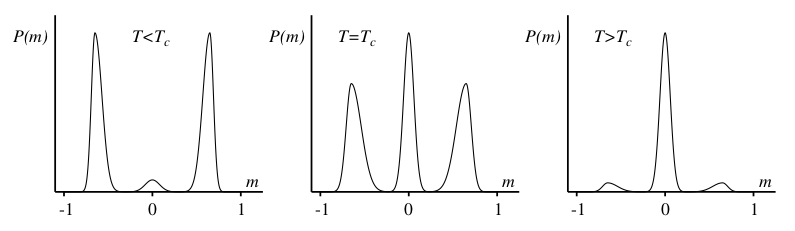
\includegraphics[scale=0.5]{fig18}
\caption{Эволюция (схема) распределения намагниченности конечного ферромагнетика Изинга, близкого к переходу первого рода. Происходит быстрый перенос веса между центральным пиком (соответствующим неупорядоченной фазе) и двумя пиками при ненулевой намагниченности (два ферромагнитных состояния), когда температура регулируется в переходной области. Пики становятся дельта-функциями в пределе бесконечного размера системы. Температуру перехода T c можно определить как точку с некоторой специфической (но по существу произвольной) характеристикой трех пиков, например равной массой или равной высотой пиков.}
\label{}
\end{figure}

Окно перехода, в котором можно наблюдать распределение из трех пиков, быстро сужается с увеличением размера системы, а пики превращаются в дельта-функции. Когда вес между пиками становится очень маленьким, на практике может оказаться невозможным эргодически сэмплировать конфигурации, так как система оказывается в ловушке внутри подпространства, соответствующего только одному из пиков.

Тип распределения параметра порядка на рис. 18 не применим к управляемому полем переходу первого рода модели Изинга с кривыми намагничивания, показанными на рис. 10. В этом случае было бы всего два пика с перенос веса между ними при настройке поля через $h = 0$. Сосуществование фаз при $h = 0$ (и $T <T_c$) соответствует двум симметричным пикам в распределениях на рис. 12. Сходство между этим случаем и парамагнетиком -магнитный переход (с общим n-компонентным параметром порядка m) может быть прояснен, если рассмотреть одномерное распределение $|m|$. Это распределение имеет два пика, один при $| m | = 0$ и один при $| m | > 0$, когда сосуществуют упорядоченная и неупорядоченная фазы. Еще раз отметим, что при непрерывных переходах (рис. 12) центральный пик непрерывно расщепляется на два пика ниже $T_c$, в отличие от двух пиков упорядочения, возникающих при ненулевом значении $|m|$ в случае первого порядка.

Соотношение Биндера, уравнение (~\ref{eq_77}) в случае общего n-мерного параметра порядка зависит только от распределения $|m|$. Он имеет очень интересное свойство при переходе первого рода. Легко проверить, используя, например, идеализированное распределение сосуществования типа $P(|m|) = (1 - p) G (| m |) + p\delta (| m | - m^{∗})$, где $G$ является нормализованным «полугауссовым» (определенным для $| m | ≥ 0$) и $0 <m^{∗} ≤ 1$, то $U_2$ демонстрирует отрицательную дивергенцию, когда вес p упорядоченной фазы настроен от $0$ до $1$, и если ширина гауссиана обращается в нуль (соответствует бесконечному размеру системы). Хотя полное m-распределение, конечно, содержит больше информации, обнаружение окна отрицательного кумулянта Биндера и проверка расхождения пикового значения может быть практическим способом анализа перехода первого рода.

\subsubsection{Модель Изинга с фрустрированной двумерной квадратной решеткой}
Здесь мы рассмотрим частный пример перехода первого рода в модели Изинга с фрустрированной двумерной квадратной решеткой с гамильтонианом

\begin{equation}
E_\sigma = -J_1\sum\limits_{\langle ij \rangle _1} \sigma_i \sigma_j + J_2\sum\limits_{\langle ij \rangle _2}\sigma_i \sigma_j
\label{eq_79}
\end{equation}

где обе связи $J_1, J_2 > 0$ (но обратите внимание на разные знаки перед параметрами).
Тогда первый член (где $\langle ij \rangle _1$ обозначает спины ближайшего соседа) является стандартным ферромагнетиком Изинга, тогда как второй член (где $\langle ij \rangle _2$ относится к спинам следующего ближайшего соседа, т. е. поперек диагоналей на плакетках $2 × 2$, как на рис.7) является антиферромагнитным и вызывает фрустрацию. Для отношений связи $g = J_2 / J_1 <1/2$ основное состояние системы является ферромагнитным (полностью поляризованным). В пределе $g → ∞$ система сводится к двум развязанным антиферромагнетикам с четырьмя полосатыми (или коллинеарными) основными состояниями, такими как показанное на рис. 7 (c). Они остаются основными состояниями при всех $g> 1/2$. В точке $g = 1/2$ основное состояние сильно вырождено. Отметим, что случай $J_1 <0$ эквивалентен $J_1> 0$, благодаря инвариантности $E_\sigma$  относительно преобразования $\sigma_i → -\sigma_i$ на одной из подрешеток шахматной доски; таким образом, в этом случае ферромагнитная фаза заменяется антиферромагнитной, а полосатая фаза не изменяется.
Фрустрированная модель Изинга изучалась давно, но некоторые особенности ее фазовой диаграммы все еще обсуждаются или были решены только недавно ~\cite{pre_80_051117, phys_145_012051, prl_108_045702}. Для $g <1/2$ переход относится к стандартному типу Изинга, но его трудно изучать вблизи $g = 1/2$ из-за больших масштабных поправок и большого времени автокорреляции Монте-Карло. Здесь мы будем рассматривать только $g> 1/2$, для которого существует переход первого рода между высокотемпературным парамагнетиком и низкотемпературной полосатой фазой, вплоть до связи $g^{∗} \approx 0,8$ ~\cite{prl_108_045702}, после чего переход становится непрерывным . Мы анализируем результаты, полученные стандартным однократным выполнением алгоритма Метрополиса (поскольку кластерные методы Монте-Карло не работают при наличии фрустрации). Температуры будут указаны в единицах $J_1$.

~\emph{Распределение параметров порядка}

Полосы упорядоченной фазы могут быть ориентированы либо по оси $x$, либо по оси $y$, с соответствующими параметрами порядка

\begin{equation}
m_x=\frac{1}{N}\sum\limits_{i=1}^N \sigma_i(-1)^{x_i}
\label{eq_80}
\end{equation}

\begin{equation*}
m_y=\frac{1}{N}\sum\limits_{i=1}^N \sigma_i(-1)^{y_i}
\end{equation*}

где $x_i$ и $y_i$ - (целые) координаты решетки узла i. Давайте сначала посмотрим на распределение параметра порядка $P(m x, m y)$. Если четыре возможных упорядоченных состояния отбираются одинаково ниже $T_c$, распределение должно быть четырехкратно симметричным с пиками, расположенными
на отрицательной и положительной оси X и Y. В парамагнитной фазе должен быть единственный центральный пик. Следовательно, сосуществование при переходе первого рода должно отражаться в наличии пяти пиков в этом случае (вместо распределения из трех пиков для параметра скалярного порядка на рис.18). На рис. 19 показаны результаты для системы $L = 128$ при $g = 0,55$ для трех температур в переходном окне. Во всех случаях можно увидеть отчетливую четырехгранную симметрию. Четыре симметричных пика четко указывают на упорядоченную фазу при $T = 0,771$, но есть сильные флуктуации, отраженные в весе, простирающемся к центру распределения.

\begin{figure}[htp]
\centering
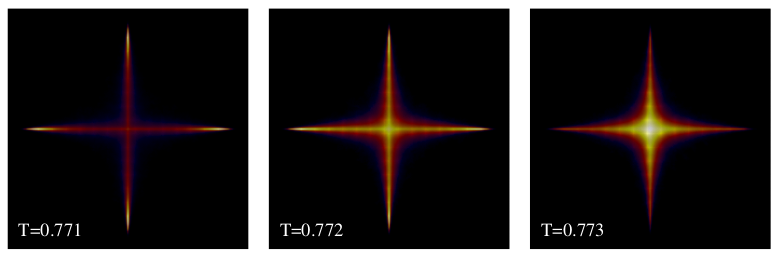
\includegraphics[scale=0.5]{fig19}
\caption{Распределения параметров порядка в плоскости $(m_x, m_y)$ (в полном пространстве $| m x | ≤ 1$, $| m y | ≤ 1$) двумерной фрустрированной модели Изинга размера $L = 128$ при коэффициенте связи $g = 0,55$. Более яркие черты соответствуют более высокой плотности вероятности. Температуры (указанные на панелях в единицах $J_1$) находятся в переходной области первого рода, причем сосуществование фаз (центральный пик, а также четыре пика, соответствующие полосам, ориентированным по оси x и y), наиболее отчетливо видны при $g = 0,772$.}
\label{}
\end{figure}


При $T = 0,773$ максимум распределения находится в центре, но вес также распространяется далеко в упорядоченные области. Между этими температурами при $T = 0,772$ можно различить как четыре пика упорядочения, так и центральный пик. Все эти сюжеты показывают отличительные черты сосуществования; даже когда нет пяти пиков, все еще существует значительная вероятность как для упорядоченных, так и для парамагнитных конфигураций. Вдали от узкого переходного окна распределение быстро превращается в одно с четко упорядоченными или неупорядоченными чертами.

~\emph{Связующее кумулянт}

Давайте проанализируем кумулянт Биндера, используя $m_2 = m_x^2 + m_y^2$ в уравнении (~\ref{eq_77}). Теперь вопрос в том, какую размерность параметра порядка n использовать в этом определении. При высоких температурах колебания $m_x$ и $m_y$ в разных частях большой системы некоррелированы. Это подразумевает вращательно-симметричное (круговое) распределение $P(m_x, m_y)$. Зависимые от n коэффициенты предназначены для того, чтобы сделать $U_2 → 0$ при $T → ∞$, и в этом случае мы должны использовать $n = 2$. Это верно также при низких температурах (чтобы гарантировать $U_2 → 1$), потому что в упорядоченном фаза отношение связующего, уравнение. (76), $R_2 → 1$, когда размер системы расходится, независимо от структуры параметра порядка. Рис.20 показывает результаты как функция температуры при двух отношениях связи; $g = 0,55$ и $0,70$. Для $g = 0,55$ отрицательный кумулянт Биндера можно увидеть при $L ≥ 8$, при этом отрицательные пики становятся очень узкими и очевидно расходятся по мере увеличения размера системы. При $g = 0,70$ переход все еще является первым порядком, но с более слабыми разрывами, которые начинают проявляться как сосуществование и отрицательный кумулянт Биндера только около размера $L = 32$. В обоих случаях моделирования Монте-Карло все еще были эргодичными, но необходимо было выполнить большое количество обновлений разверток ($\approx 10^8$ для каждого случая) для получения гладких кривых.

\begin{figure}[htp]
\centering
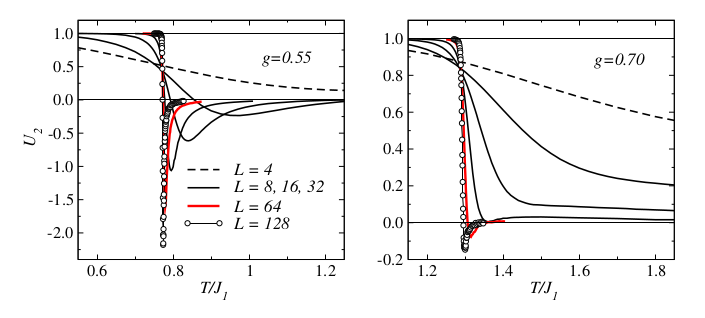
\includegraphics[scale=0.5]{fig20}
\caption{Кумулянт связующего при переходе к полосатой фазе фрустрированной модели Изинга для соотношений связи $g = 0,55$ (слева) и $g = 0,70$ (справа). Расходящийся отрицательный пик, развивающийся с увеличением $L$, является однозначным сигналом перехода первого рода.}
\label{}
\end{figure}

~\emph{Разрывы и масштабирование конечных размеров.}

В переходах первого рода, которые не очень сильны, как в системах выше, может быть нелегко точно определить размер разрывов в физических наблюдаемых. Пример показан на рис. 21, где график зависимости внутренней энергии от температуры для нескольких размеров решетки. Хотя при увеличении L явно возникает разрыв (скрытая теплота), нелегко точно определить, между какими двумя энергиями в конечном итоге произойдет скачок. Это требует тщательного анализа с использованием более крупных решеток.

\begin{figure}[htp]
\centering
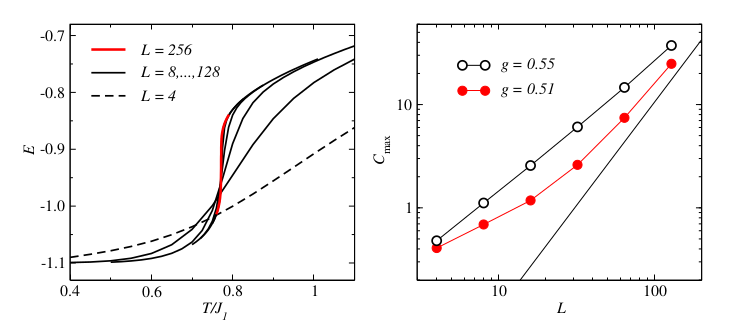
\includegraphics[scale=0.5]{fig21}
\caption{Слева: внутренняя энергия в зависимости от температуры для фрустрированной модели Изинга при $g = 0,55$. Разрыв, развивающийся с увеличением размера решетки, соответствует скрытой теплоте. Справа: шкала конечных размеров пикового значения теплоемкости при $g = 0,51$ и $0,55$. Линия показывает ожидаемое асимптотическое масштабирование $L^2$ при переходе первого рода.}
\label{}
\end{figure}

На рис. 21 также показано максимальное значение удельной теплоемкости в зависимости от размера системы для двух различных соотношений сцепления. При $g = 0,51$ переход является довольно сильным переходом первого рода, и для самых больших решеток может наблюдаться масштабирование, соответствующее ожидаемому $C_max \approx L^2$. Напротив, при $g = 0,55$ поведение, по-видимому, следует другому степенному закону (с показателем, близким к 1,2) вплоть до $L \approx 64$. Однако для больших решеток результаты начинают показывать несколько более быстрое расхождение, и в конечном итоге для очень больших решеток, можно было бы ожидать, что показатель степени будет равен $d = 2$ и в этом случае.

\subsection{Спиновая жесткость и переход Костерлиз-Таулесс}
Важным аспектом системы с дальним магнитным порядком является то, что она демонстрирует ненулевую спиновую жесткость. Для системы с непрерывными векторными спинами (модели XY или Гейзенберга) спиновая жесткость является аналогом модуля упругости твердого тела. Также часто называется модулем спиральности ~\cite{pra_8_1111}. 
Чтобы изучить эту концепцию, мы рассмотрим $XY$-модель с гамильтонианом, записанным  как:

\begin{equation}
H = -J\sum\limits_{\langle i,j \rangle} cos(\Theta_i - \Theta_j)
\label{eq_81}
\end{equation}

где $\Theta_i \in [0, 2\pi]$ - угол, характеризующий спин i. Для простоты мы предполагаем только взаимодействия ближайших соседей, но обобщения на произвольные взаимодействия очевидны. При выводе выражения для спиновой жесткости мы будем рассматривать двумерную квадратную решетку (и иногда для простоты использовать одномерную цепочку), но позже изучим также трехмерную кубическую систему. В 2D XY-системах спиновая жесткость является важной величиной, характеризующей нетрадиционный (топологический) переход Костерлица-Таулеса, проявляемый этой системой, который мы также кратко обсудим в этом разделе.

\subsubsection{Определение спиновой жесткости}
Грубо говоря, спиновая жесткость $\rho_s$ характеризует тенденцию упорядоченных спинов к адаптации в ответ на возмущения, вызывающие модуляцию направления параметра порядка (в отличие от восприимчивости, которая измеряет тенденцию изменения параметра порядка под действием поля применяется в фиксированном направлении). Он аналогичен модулю сдвига в механике сплошной среды, который характеризует тенденцию к деформации формы упругого объекта (в то время как сжимаемость соответствует тенденции к изменению объема при сохранении формы). Определение спиновой жесткости легче всего понять при $T = 0$, которое мы рассмотрим сначала, прежде чем обобщать на $T> 0$.

~\emph{Жесткость при $T = 0$. }
Сначала мы рассмотрим систему с открытыми границами в направлении $x$. На рис.22 показано, как ферромагнитные спины $XY$ при $T = 0$ адаптируются для минимизации энергии, когда накладывается общее изменение угла спина $\phi$ между левой и правой границами (например, из-за сильных магнитных полей, приложенных к границе столбцы). 

\begin{figure}[htp]
\centering
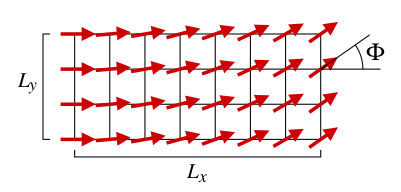
\includegraphics[scale=0.5]{fig22}
\caption{Двухмерная классическая XY-модель с фазовым сдвигом в направлении $x$, наложенным путем фиксации спинов в граничном столбце под относительным углом $\Phi$. Чтобы минимизировать энергию, полное скручивание $\Phi$ распределяется равномерно, так что спины в соседних столбцах скручены на $\phi = \Phi / L_x$ относительно друг друга.}
\label{}
\end{figure}

Чтобы минимизировать энергию, каждый столбец развернут относительно следующего столбца на угол $\phi = \Phi / (L_x - 1)$, где $L_x$ - длина системы в направлении x (количество столбцов). При $T = 0$ нас интересует энергия при наличии этого разворота, которая для 2D $XY$-модели дается выражением:

\begin{equation}
E(\phi) = -J(L_x-1)L_y cos(\phi) = E(0)+J(L_x - 1)L_y[1-cos(\phi)]
\label{eq_82}
\end{equation}

Для малых $\phi$ получаем $E (\phi) - E (0) = (J / 2) (L_x - 1) L_y \phi^2$ в старшем порядке. На основании этого результата спиновая жесткость T = 0 определяется как

\begin{equation}
\rho_s = \frac{1}{N}\frac{\partial^2 E(\phi)}{\partial\phi^2}
\label{eq_83}
\end{equation}

и у нас есть $\rho_s = J$ для больших N [или для любого N, если мы нормируем на число $L_y (L_x - 1)$ взаимодействующих x-связей, по которым распределяются затраты энергии из-за скручивания].

Обычно удобнее рассматривать периодическую систему. Чтобы получить выражение для спиновой жесткости в этом случае, сначала на границе накладывается фазовый сдвиг. Для простоты мы прорабатываем это для одномерной цепочки с углами спина $\Theta_x$, $x = 0,\dots, N - 1$, но вычисление можно тривиально обобщить на более высокую размерность. Энергия взаимодействия для каждой связи равна $E_x = −J cos (\Theta_{ x + 1} - \Theta_x)$, за исключением границы, где скрутка $\Phi$ соответствует $E_N = −J cos (\Theta_0 − \Theta_{N − 1} + \Theta)$ . Конфигурации, минимизирующие энергию, имеют $ \Theta_{x + 1} - \Theta_x = \delta$, где $\delta$ не зависит от $x$, что дает полную энергию

\begin{equation}
E(\Phi) = -(N-1)cos(\delta)-cos(\Phi-[N-1]\delta)
\label{eq_84}
\end{equation}

которое минимизируется соотношением $\delta = \phi \equiv \Phi / N$, где $E (\phi) = E (0) + JN [1 - cos (\phi)]$, а спиновая жесткость, определенная согласно (83), снова равна $\rho_s = J$

Полезно рассмотреть еще один способ разворота спинов в периодической системе, введя в гамильтониан закручивающее поле $\Phi_x = x\phi$. Для одномерной системы энергия каждой связи в присутствии этого поля равна $−J cos (\Theta_{x + 1} - \Theta_x + \Theta_{x + 1} - \Theta_x)$. Чтобы правильно рассматривать границу, $\Theta_x$ следует рассматривать как функцию непрерывной переменной $x$, скачкообразно меняющейся от $N\phi$ до 0 при $x = N$. Разность фаз, возникающая во взаимодействии $XY$, должна тогда интерпретироваться как

\begin{equation}
\Phi_{x+1}-\Phi_x= \int_{x}^{x+1}\Phi_x dx = \int_{x}^{x+1}\phi dx = \phi
\label{eq_85}
\end{equation}

что имеет место и на границе $(x + 1 = N)$. $\phi$ аналогичен потоку, пронизывающему кольцо. Энергия при наличии этого скручивания минимизируется для $\Theta_x = \Theta$ независимо от $x$, что дает $E(\phi) = E(0) + JN [1 - cos (\phi)]$, как и раньше в случае скрученного граничного условия. 

~\emph{Жесткость при T>0}

Теперь рассмотрим ненулевые температуры, и в этом случае спиновая жесткость определяется как:

\begin{equation}
\rho_s=\frac{1}{N}\frac{\partial^2F(\phi)}{\partial \phi^2}
\label{eq_86}
\end{equation}

где $F (\phi)$ - свободная энергия при наличии закручивающего поля (или, что то же самое, скрученного граничного условия), которая, в свою очередь, связана со статистической суммой согласно:

\begin{equation}
F(\phi)=-\frac{1}{\beta}ln(Z(\phi))
\label{eq_87}
\end{equation}

При $T \to 0$ уравнение (~\ref{eq_86}) явно сводится к определению энергии основного состояния (~\ref{eq_83})

Применяя скручивающее-поле, которое зависит только от $x, \Phi(x, y) = x\phi$, в 2D XY-модели, мы получаем гамильтониан

\begin{equation}
H(\phi) = -J\sum\limits_{\langle i,j \rangle _x}cos(\phi + \Theta_j - \Theta_i) -J\sum\limits_{\langle i,j \rangle _x}cos(\Theta_j - \Theta_i)
\label{eq_88}
\end{equation}

где мы можем предполагать периодические граничные условия в обоих направлениях (хотя в принципе граница y может быть открытой). Мы можем упростить зависимость от $\phi$, используя стандартное тригонометрическое равенство

\begin{equation}
cos(\phi + \Theta_j - \Theta_i)=cos(\Theta_j - \Theta_i)cos(\phi)-sin(\Theta_j - \Theta_i)sin(\phi)
\label{eq_89}
\end{equation}

который мы разложим до второго порядка по $\phi$:

\begin{equation}
cos(\phi + \Theta_j - \Theta_i) \to cos(\Theta_j - \Theta_i)(1-\phi^2)-sin(\Theta_j - \Theta_i)\phi + O(\phi^3 )
\label{eq_90}
\end{equation}

Тогда гамильтониан при наличии небольшой $(\phi to 0)$ закрутки можно записать как:

\begin{equation}
H(\phi) \to H(0)+\frac{1}{2}\phi^2H_x-\phi I_x
\label{eq_91}
\end{equation}

где $H_x$ - это часть гамильтониана, связанная с x, при $\phi = 0$, а $I_x$ - полный спиновый «ток» в направлении решетки $x$:

\begin{equation}
I_x = J \sum\limits_{\langle i,j \rangle_x}sin(\Theta_j-\Theta_i)
\label{eq_92}
\end{equation}

Статистическая сумма при наличии небольшого поворота может быть записана как

\begin{equation}
Z(\phi)=\int d[\Theta]e^{-\beta H(\phi)} \to \int d[\Theta]e^{-\beta H(0)}[1-\frac{1}{2}\beta\phi^2 H_x + \dots][1+\beta\phi I_x + \frac{1}{2}(\beta\phi I_x)^2  + \dots ]
\label{eq_93}
\end{equation}

где экспоненты, включающие $H_x$ и $I_x$, были расширены по Тейлору до необходимых порядков. Теперь мы можем записать это в форме с математическими ожиданиями по распределению для $\phi = 0$. Для второго порядка по $\phi$:

\begin{equation}
Z(\phi) \to Z(0)[1-\frac{1}{2}\beta\phi^2\langle H_x \rangle + \beta \phi \langle I_x \rangle + \frac{1}{2}\beta^2\phi^2 \langle I_x^2 \rangle] 
\label{eq_94}
\end{equation}

В силу симметрии $\langle I_x \rangle = 0$, а свободная энергия (~\ref{eq_87}) определяется выражением

\begin{equation}
F(\phi) = F(0)+\frac{1}{2}\phi^2(\langle H_x \rangle -\beta \langle I_x^2 \rangle )
\label{eq_95}
\end{equation}

и отсюда можно извлечь простое выражение для спиновой жесткости (~\ref{eq_86}):

\begin{equation}
\rho_s = \frac{1}{N}(\langle H_x \rangle - \beta \langle I_x^2 \rangle)
\label{eq_96}
\end{equation}

которые можно оценить с помощью моделирования Монте-Карло. Этот результат относится к закручивающему полю в направлении решетки x. Для d-мерной изотропной системы мы можем усреднить по всем эквивалентным направлениям и записать спиновую жесткость как

\begin{equation}
\rho_s = \frac{1}{Nd}(\langle H \rangle - \beta \sum\limits_{\alpha=1 }^{d} \langle I_{\alpha}^2\rangle)
\label{eq_97}
\end{equation}

где индекс $\alpha$ соответствует току в направлении решетки $\alpha$. Для анизотропной d-мерной системы жесткость в общем случае различна для всех направлений решетки, то есть существует d различных констант жесткости, каждая из которых задается формой, подобной (~\ref{96}).

Определение жесткости с помощью крутящего-поля можно легко обобщить на системы с дальнодействующими взаимодействиями. Формы (~\ref{96}) и (~\ref{97}) остаются в силе, при этом ток $I_x$ содержит вклады от всех взаимодействий точно так же, как в гамильтониане.

Отношение к сверхтекучести и сверхпроводимости

Очень интересным аспектом спиновой жесткости модели XY является то, что она может быть напрямую связана со сверхтекучей плотностью сверхпроводника (или сверхтекучей жидкости, такой как  He$^4$) [131, 132]. Как и намагничивание в модели XY, параметр порядка сверхпроводника или сверхтекучей жидкости является $U (1)$ -симметричным (соответствует глобальной фазе волновой функции), а закручивающее поле, которое мы обсуждали выше, прямо аналогично магнитному потоку ( в случае сверхпроводника). Ненулевая жесткость соответствует эффекту Мейснера сверхпроводника. Моделирование методом Монте-Карло двумерной XY-модели, непосредственно направленное на изучение свойств тонких сверхтекучих пленок, обсуждается в работах [1,96]. [133, 134].

Масштабирование спиновой жесткости

Критические масштабные свойства спиновой (или сверхтекучей) жесткости были впервые разработаны в контексте сверхтекучих жидкостей [131, 132]. В бесконечной d-мерной системе с $d> 2$ было показано, что

\begin{equation}
\rho_s \sim (T_c - T)^{(d-2)\nu }
\label{eq_98}
\end{equation}

для $T \to T_c$. Здесь $\nu$ - стандартный показатель корреляционной длины. В соответствии с общим масштабным соотношением конечных размеров (~\ref{eq_66}) зависимость жесткости от размера точно при T c определяется выражением

\begin{equation}
\rho_s \sim L^{2-d}
\label{eq_99}
\end{equation}

Таким образом, жесткость, как длина корреляции и коэффициент Биндера (Binder), является полезной величиной для определения критической точки без необходимости корректировки каких-либо неизвестных (или не совсем известных) показателей. Это проиллюстрировано результатами Монте-Карло для трехмерной XY-модели на рис. 23, где $L\rho_s$ не зависит от размера в критической точке.


\subsubsection{Переход Костерлиз-Таулесс в двух измерениях}
В 2D XY-модели не может быть перехода в фазу с дальним магнитным порядком при T> 0, согласно теореме Мермина-Вагнера [38] (как обсуждалось в разделе 2).

Примечательно, что в этой системе наблюдается фазовый переход другого типа, при котором дальний порядок не развивается, но спиновые корреляции меняются от экспоненциально затухающей до степенной [135, 136]. Этот переход Костерлица-Таулеса (КТ) имеет топологическую природу, являясь следствием распространения несвязанных вихрей (которые являются топологическими дефектами) в спиновых конфигурациях при температурах $T> T_{KT}$. При $T \le T_{KT}$ вихри также существуют (с плотностью, которая обращается в нуль при $T \to 0$), но все они связаны парами вихрь-антивихрь, которые не имеют чистой завихренности (и, следовательно, исчезают при постепенном измельчении спинов). Степенная форма спиновых корреляций $C(r) \sim r^{- \eta}$ применима для всех $0 < T \le T_{KT}$. 
Показатель $\eta$ зависит от температуры, при этом значение $\eta = 1/4$ точно при $T_{KT}$ и $\eta \to 0$ при $T \to 0$, так что истинный дальний порядок существует при $T$

Хотя для $0 <T \le T_{KT}$ нет длинного порядка, спиновая жесткость на самом деле отлична от нуля в фазе $KT$ - степенная корреляция с достаточно малым показателем степени достаточно, чтобы поддержать энергетические затраты на скручивание границы. Нет никакого степенного начала жесткости, но вместо этого есть еще более заметный сигнал перехода; скачок при $T_KT$ от $\rho_s = 0$ до ненулевого значения. Расчеты ренормгруппы для теории поля континуума, соответствующей 2D XY-модели, дали очень подробную информацию о KT-переходе. Одним из наиболее важных результатов является строгая связь (полученная Нельсоном и Костерлизом [139]) между температурой перехода $T_{KT}$ и спиновой жесткостью именно при этой температуре (т.е. размером разрыва);

\begin{equation}
\rho_s(T_{KT})=\frac{2T_{KT}}{\pi} 
\label{eq_100}
\end{equation}

Для конечных решеток жесткость при T KT приближается к значению бесконечного размера с логарифмической поправкой на размер [138]:

\begin{equation}
\rho_s(T_{KT}, L)=\rho_s(T_{KT}, \infty)(1+\frac{1}{2ln(L)+c})
\label{eq_101}
\end{equation}

где $c$ - системно-зависимый параметр. Таким образом, можно сказать, что общий закон масштабирования конечного размера (~\ref{eq_99}) для $\rho_s$ в критической точке выполняется, но с логарифмической поправкой к не зависящей от размера форме в главном порядке, получаемой при $d = 2$.

На рис. 24 (а) показаны результаты Монте-Карло для жесткости 2D XY-модели в зависимости от температуры. Скачок, ожидаемый в термодинамическом пределе, достигается очень медленно в зависимости от размера. Это может быть связано с тем, что корреляционная длина при $T> T_{KT}$ расходится не по степенному закону, а по экспоненциальной форме

\begin{equation}
\xi \sim e^{\frac{a}{\sqrt{T-T_{KT}}}}
\label{eq_102}
\end{equation}

где a зависит от деталей решетки и взаимодействий. Поэтому, используя те же аргументы, что и в случае стандартной критической точки в п. 3.3.2, конечный сдвиг $T_{KT}$ [определяемый, например, с помощью температуры $T ∗ (L)$, при которой $\rho_s$ падает наиболее быстро], задается формой,

\begin{equation}
T^{*}(L)-T_{KT} \sim \frac{1}{ln^2(L)}
\label{eq_103}
\end{equation}

что намного медленнее, чем обычный степенной сдвиг $T^{*} - T_{KT} \sim L^\frac{1}{\nu}$

Используя стандартную гипотезу масштабирования конечных размеров (~\ref{eq_64}) и заменяя $L^{\sigma}$ (размерная зависимость сингулярной величины точно в критической точке) логарифмической поправкой на размер в (~\ref{eq_101}), мы можем записать гипотезу для размерной и температурной зависимости спиновой жесткости на переходе KT как

\begin{equation}
\rho_s(T,L)=(1+\frac{1}{2ln(L)+c})f(e^{a/(T-T_{KT})^{1/2}}/L)
\label{eq_104}
\end{equation}

которое после логарифмирования аргумента масштабирующей функции f (x) может быть записано в терминах другой функции g [ln (x)] как

\begin{equation}
\rho_s(T,L)(1+\frac{1}{2ln(L)+c})^{-1} = g[ln(L)-\frac{a}{\sqrt{T-T_{KT}}}]
\label{eq_104}
\end{equation}

Здесь $T \to T_{KT}$ соответствует аргументу $ln(L)-\frac{a}{\sqrt{T-T_{KT}}} \to -\infty$

\begin{figure}[htp]
\centering
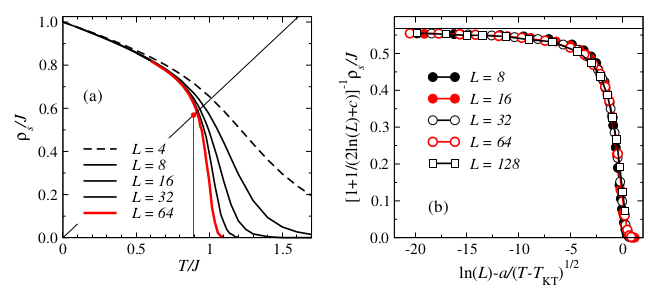
\includegraphics[scale=0.5]{fig24}
\caption{(а) Результаты Монте-Карло (полученные с помощью кластерного алгоритма ~\cite{prl_62_361} ) для температурной зависимости спиновой жесткости 2D XY-модели для нескольких решеток размером $L = 2^n$. Разрыв возникает при $T_{KT}$ при $L \to \infty$, как показано вертикальной линией при известной температуре перехода ($T_ KT \approx 0,8933$ ~\cite{prb_65_184405}). Согласно соотношению Нельсона-Костерлица (~\ref{eq_100}), жесткость точно при $T_{KT}$ для любой системы, демонстрирующей KT-переход, должна попадать в показанную линию; $\rho_s = 2T / \pi$. (b) Коллапс данных конечного размера в соответствии с гипотезой комбинированного (T, L) масштабирования (~\ref{eq_105}) с использованием известного T KT = 0,8933 и двух параметров, $a = 1,5$ и $c = 0,7$, выбранных для получения хорошего коллапса данных. Вертикальная линия показывает асимптотическое значение $T \to T_{KT}$, $L \to \infty $, ожидаемое согласно соотношению Нельсона-Костерлица.}
\label{}
\end{figure}

Температура KT-перехода 2D XY-модели была извлечена различными способами во многих исследованиях, например, в ~\cite{prb_49_12071, prb_65_184405} . На рис. 24 (b) показан тест масштабной формы (~\ref{eq_105}) с использованием $T_{KT} = 0,8933$, полученного в ~\cite{prb_65_184405} , и с константами $a$ и $c$, скорректированными для получения (приблизительно) наилучшего сворачивания данных на общий функция масштабирования для размеров системы $L = 8, 16,. . ., 128$. Данные действительно хорошо описываются этой формой. Этот вид графика подтверждает три различных аспекта перехода KT (которые были теоретически выведены на разных этапах истории перехода KT) одновременно; экспоненциально расходящаяся корреляционная длина (~\ref{eq_102}) ~\cite{phys_6_1181, phys_7_1046}, логарифмическая поправка (~\ref{eq_101}) ~\cite{prb_37_5986} и соотношение Нельсона-Костерлица (~\ref{eq_100}) ~\cite{prb_39_1201} .

\subsection{Квантовые фазовые переходы}

В следующих разделах будет приведено несколько примеров квантовых фазовых переходов, которые происходят в основном состоянии системы в зависимости от некоторого параметра модели ~\cite{sachdev}. Свойства масштабирования, которые были обсуждены выше для классических непрерывных переходов и переходов первого рода, все еще применимы с некоторыми важными расширениями и модификациями. Природу классического теплового фазового перехода можно объяснить особенностями свободной энергии. При квантовом фазовом переходе энергия основного состояния демонстрирует сингулярное поведение, которое проявляется и в других величинах. Это можно понять как возникающую из-за свободной энергии $T> 0$ квантовой системы, которая при $T \to 0$ становится энергией основного состояния. Это, конечно, также верно и в классическом смысле, но основные состояния классических моделей обычно не развиваются непрерывно в зависимости от параметров (как мы видели на примере фрустрированной модели Изинга в разделе 3.4.2) и, следовательно, являются строго первого порядка. Напротив, как уже обсуждалось в разд. 2.4, квантовые системы имеют нетривиальные основные состояния с нулевыми флуктуациями, которые развиваются при изменении параметров. Обычны непрерывные фазовые переходы, вызванные расходящимися квантовыми флуктуациями.

Квантовая d-мерная  система может быть формально отображена, используя интегралы по путям, в эквивалентную задачу классической статистической механики в $d + 1$ измерениях (хотя иногда и с неположительно определенной функцией распределения). Размер системы в новом измерении «мнимого времени» - это обратная температура; $L_{\tau} = c / T$, где c - скорость. При $T> 0$ эта размерность конечна, а пространственные размеры могут быть бесконечными. Тогда система будет d-мерной с «толщиной» $L_{\tau}$. Строгая $(d + 1)$ -мерность применяется, когда также $T \to 0$. В этом случае настраиваемый параметр в гамильтониане может играть роль, очень похожую на температуру в классической системе. Интересно, что изменение температуры в этом случае аналогично масштабированию конечных размеров в $L_{\tau}$ ~\cite{prb_39_2344}, которое может использоваться для вывода свойств масштабирования при конечных температурах вблизи квантово-критических точек ~\cite{prb_49_11919}.

В некоторых случаях d-мерная квантовая система обладает низкоэнергетическими свойствами того же типа классической системы в d +1 измерениях. Так обстоит дело, например, с димеризованными моделями Гейзенберга, обсуждаемыми в гл. 2.4. Физика низких энергий этих моделей может быть отображена на трехмерной классической модели Гейзенберга, что обычно делается с помощью теорий континуального поля, таких как нелинейная $\sigma$-модель ~\cite{prb_39_2344, prb_49_11919} (и, следует отметить, димеризация является лишь средством настройки силы квантовых флуктуаций, которая в крупномасштабной однородной эффективной модели просто представлена ​​константой связи теории поля или температурой в эффективной трехмерной однородной классической модели ~\cite{pss_241_2118}). Тогда можно предположить, что квантовый фазовый переход, вызванный настройкой силы димеризации, должен быть в классе универсальности управляемого температурой перехода трехмерной классической модели Гейзенберга. В других случаях низкоэнергетическое отображение может дать эффективную систему, которая не соответствует какой-либо известной классической модели, но все же можно сказать, что система соответствует некоторой $(d + 1)$ -мерной эффективной модели.

~\emph{Динамический критический показатель.}

Во многих случаях, таких как димеризованные модели Гейзенберга, упомянутые выше, временное измерение, возникающее при отображении в d +1 измерений, эквивалентно (в асимптотическом смысле) пространственным измерениям. Масштабные свойства такой системы при квантовом фазовом переходе тогда получаются простой заменой $d$ на $d + 1$ в критической корреляционной функции (~\ref{eq_53}), в соотношениях гипермасштабирования, таких как второе уравнение. (~\ref{eq_59}), а в скалиновых формах (~\ref{eq_98}) и (~\ref{eq_99}) спиновой жесткости. В других случаях корреляции в новом измерении могут принципиально отличаться от корреляций в пространственных измерениях. Динамический показатель z связывает степенные законы, связанные с пространственными и временными корреляциями, например, если длина пространственной корреляции $\xi$ расходится, когда некоторый параметр g настроен на свое критическое значение как $| g - g_c |^{ −1 / \nu}$, то временная корреляционная длина расходится как $| g - g_c |^{ z / \nu}$, а в классических калибровочных соотношениях следует заменить d на $d + z$ для квантовой критической точки.

Динамический показатель получил свое название от того факта, что он также определяет дисперсию $\omega(q) \sim q^z$ возбуждений с волновым числом q. Важным аспектом этого является то, что щель возбуждения конечного размера получается установкой $q \propto 1/ L$, что дает масштабирование щели $\Delta_L ∼ 1 / L^z$. Этот результат можно использовать непосредственно в численных расчетах, а также имеет косвенные последствия для масштабных свойств величин, которые зависят от спектра возбуждения (например, различных восприимчивостей). Извлечение динамического показателя является важным аспектом вычислительных исследований квантовых фазовых переходов. Помимо этого, квантовые фазовые переходы, как непрерывные, так и переходы первого рода, можно анализировать с помощью тех же методов масштабирования конечных размеров, что и классические переходы, обсуждавшиеся выше.

Следует отметить, что динамический показатель присутствует также в классических системах, но он не играет роли в равновесной статистической механике (потому что, если система имеет кинетическую часть гамильтониана, соответствующее распределение вероятностей в фазовом пространстве сокращает в ожидаемых значениях). Классический динамический показатель зависит от того, как динамика вводится в систему ~\cite{prb_13_1299}. Алгоритм Метрополиса Монте-Карло для модели Изинга является примером классической динамики (называемой глауберовской
динамика), а длительное затухание автокорреляций при критичности регулируется соответствующим динамическим показателем. Однако эта динамика не определяет равновесные свойства. В квантовой механике динамику нельзя выделить отдельно, но она является неотъемлемой частью свойств равновесия, потому что полный гамильтониан всегда входит и содержит в себе как статические, так и динамические свойства ~\cite{prb_69_315}.

\section{Точные методы диагонализации}
Путем точной диагонализации гамильтониана можно получить полное представление о квантовой спиновой системе - с доступными собственными состояниями можно вычислить любую статическую или динамическую величину. В принципе, все собственные состояния могут быть точно вычислены для конечной квантовой системы путем построения гамильтоновой матрицы и ее численной диагонализации. Однако на практике такие точные исследования диагонализации ограничиваются довольно небольшими решетками, несколькими десятками спинов, из-за экспоненциального увеличения размера базиса с числом спинов ($2^N$ состояний в случае $S = 1/2$) . Поэтому следует проявлять большую осторожность при выводах о термодинамическом пределе, что может быть даже невозможно (если имеющиеся решетки слишком малы для того, чтобы приспособиться к физике бесконечного размера). Тем не менее, выводы, полученные в результате исследований точной диагонализации, очень полезны сами по себе и в качестве дополнения к другим расчетам. Точные результаты для малых решеток также необходимы для проверки правильности, например, квантовых программ Монте-Карло. Кроме того, методы точной диагонализации обеспечивают конкретный путь к изучению многих важных аспектов квантовой механики, в частности свойств симметрии состояний многих тел.

~\emph{Диагонализация блока.}

Учитывая гамильтониан H, первым шагом точного вычисления диагонализации является выбор базиса, в котором он и другие интересующие нас операторы будут выражены. Рабочий базис для системы со спином 1/2 обычно состоит из состояний с одним спином $↑_i$ и $↓_i$, $i = 1,\dots, N$ (направление квантования обычно принимается за z). Однако из-за роста гильбертова пространства на $2^N$ с увеличением числа спинов в системе, по возможности следует использовать симметрии, чтобы сначала привести гамильтониан к блочно-диагональной форме, как показано на рис. 25. 

\begin{figure}[htp]
\centering
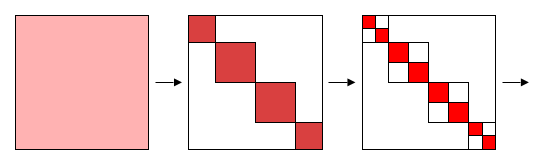
\includegraphics[scale=0.5]{fig25}
\caption{Схематическое изображение диагонализации блока. В исходном базисе гамильтониан не имеет видимой структуры (слева). Путем построения состояний, помеченных сохраняющимся квантовым числом, матрица разбивается на блоки (со всеми элементами матрицы равными нулю за пределами заштрихованных квадратов), которые можно диагонализовать независимо друг от друга (в центре). Применяя другую симметрию (закон сохранения), блоки можно разбить на более мелкие блоки (справа), помеченные двумя разными квантовыми числами и т. д.}
\label{}
\end{figure}

В такой схеме , спиновые состояния объединяются и упорядочиваются с помощью соответствующих операций симметрии. Блоки соответствуют состояниям с разными сохраняющимися квантовыми числами, связанными с симметриями, например, сохранение импульса кристалла, вытекающее из трансляционной симметрии решетки, или сохраняющаяся z-компонента полного спина (намагниченность). Блоки можно диагонализировать независимо друг от друга, что значительно снижает вычислительные затраты. В дополнение к уменьшенным вычислительным затратам, немедленный доступ к квантовым числам очень полезен для классификации возбуждений.

Некоторые симметрии относительно легко использовать в своих интересах (например, сохранение намагниченности), тогда как другие требуют некоторой дополнительной работы и приводят к более сложным базисным состояниям (например, импульсным состояниям). Некоторые симметрии, которые можно было бы использовать в принципе, обычно не реализуются, потому что практические сложности расчета могут перевесить преимущества. Примером этого является сохранение полного спина.

Использование симметрий при точной диагонализации можно обсудить на языке теории групп ~\cite{lnp_645_227}. Однако в этом формализме нет необходимости (и часто это сбивает с толку), и здесь используется более практический подход, без ссылки на терминологию теории групп. Теория групп на самом деле очень полезна при работе со сложными решетками, но силу ее формализма, возможно, можно будет лучше оценить после того, как будет получено полное понимание операций симметрии и блочной диагонализации с помощью менее формальных методов для простых решеток. Здесь мы рассматриваем одномерные цепочки и двумерные простые квадратные решетки.

\subsection{Диагонализация цепи Гейзенберга}
Изучим антиферромагнитную цепочку Гейзенберга $S = 1/2$ с гамильтонианом

\begin{equation}
H=\frac{1}{2}J\sum\limits_{i=0}^{N-1}S_iS_{i+1}=\frac{1}{2}J\sum\limits_{i=0}^{N-1}[S_i^zS_{i+1}^z+\frac{1}{2}(S_i^{+}S_{i+1}^{-} + S_i^{-}S_{i+1}^{+})]
\label{eq_106}
\end{equation}

где по причинам, которые станут очевидными ниже, здесь будет практично обозначить спины $i = 0, \dots , N - 1$. Периодические границы, $S_N = S_0$, будут предполагаться, когда мы будем рассматривать импульсные состояния, но до этого граничное условие произвольно.


\subsubsection{Представления состояний и симметрий}

~\emph{Преобразования решетки.}

Мы используем стандартные обозначения $| S_0^z,\dots, S_{N-1}^z \rangle$ для базисных z-состояний, причем $S^z$ слева направо всегда соответствует спиновым состояниям на узлах решетки, пронумерованных 0, 1, 2, $\dots$, независимо от порядка индексов $i$. Таким образом, если мы напишем состояние $| S_1^z,S_0^z  \rangle$, оно будет отличаться от $| S_0^z,S_1^z  \rangle$, если только $S_0^z=S_1^z$. Первый может относиться к состоянию, полученному из последнего, когда два спина переключаются оператором перестановки P, который может быть определен операционно так, чтобы влиять на индексы узлов; $P| S_0^z, S_1^z \rangle = | S_1^z, S_0^z \rangle$, например, $P | ↑ ↓ \rangle = | ↓ ↑ \rangle$. Обобщая это на N-спиновые преобразования решетки, отражения, трансляции и повороты (в двух и трех измерениях) определяются в терминах перестановок спиновых индексов. В качестве примера для периодической цепочки мы определяем оператор трансляции как перемещение спинов на один шаг циклически «вправо»;

\begin{equation}
T|S_0^z, S_1^z,\dots,S_{N-1}^z\rangle = |S_{N-1}^z, S_0^z,\dots,S_{N-2}^z\rangle
\label{eq_107}
\end{equation}

Это соответствует уменьшению индекса спина на единицу (модуль размера системы N) в z каждой позиции i в векторе: $S_i^z \to S_{i − 1}^z$. При записи определенных состояний со вращениями вверх и вниз, обозначенными ↑ и ↓, например, $| ↑ ↓ ↑ ↓\dots \rangle$ индексы обычно не нужны (и для компактности записи стрелки также не разделяются запятыми)

Гамильтониан Гейзенберга (~\ref{eq_106}) с периодическими граничными условиями инвариантен относительно сдвигов, т. е. коммутирует с T; $[H, T] = 0$. Следовательно, мы можем построить импульсные состояния $| \psi(k) \rangle$, которые по определению являются собственными состояниями оператора сдвига,

\begin{equation}
T| \psi (k) \rangle = e^{ik}| \psi (k) \rangle
\label{eq_108}
\end{equation}

Здесь допустимые импульсы $k = 2n \pi / N$, где $n = 0, \dots , N −1$, следующее из того, что $T^N = 1$. Состояния с разными k образуют свои индивидуально диагонализуемые блоки гамильтониана. Как на практике конструируются импульсные состояния и как они используются в компьютерной программе, будет обсуждаться в гл. 4.1.3.

Гамильтониан Гейзенберга также коммутирует с оператором отражения (четности), который мы определим способом, обобщающим уже рассмотренные двухспиновые перестановки, в терминах преобразования спинового индекса $i \to N - 1 - i$;

\begin{equation}
P|S_0^z, S_1^z,\dots,S_{N-1}^z\rangle = |S_{N-1}^z, \dots, S_1^z,S_0^z\rangle
\label{eq_109}
\end{equation}

Для собственного состояния $P, T | \psi (p) \rangle = p | \psi (p) \rangle$, где $p = \pm 1$, поскольку $P^2 = 1$. Мы будем использовать T и P для блочной диагонализации, хотя, как мы обсудим подробно в гл. 4.1.4, их нельзя всегда использовать одновременно, потому что $[T, P] = 0$ только в подпространстве гильбертова пространства. Для системы с открытыми границами T не определено, но можно использовать P.

~\emph{Спиновые квантовые числа.}

Поскольку гамильтониан спин-вращательно-инвариантен, его собственные состояния также должны быть собственными состояниями квадрата $S^2$ полного спина, где

\begin{equation}
\vec S = \sum\limits_{i=0}^{N-1 }\vec{S_i}
\label{eq_110}
\end{equation}

Для собственного состояния $\vec{S}^2 | \psi (S) \rangle = \vec{S} · \vec{S} | \psi (S) \rangle = S (S + 1) | \psi (S) \rangle $. Здесь есть вероятность путаницы, поскольку один и тот же символ S используется как для величины спина отдельных спинов (т. е. $S_i = S$), так и для полного спина состояния многих тел. Контекст всегда должен прояснять смысл (и мы в любом случае рассматриваем здесь только $S_i = 1/2$).
Мы знаем, что при сохранении полного спина состояния могут образовывать блоки, помеченные квантовыми числами $(S, m_z)$, где $m_z \in (−S, −S + 1,\dots , S)$ - полная намагниченность в направлении оси квантования,

\begin{equation}
m_z = \sum\limits_{i=0}^{N-1 }\vec{S_i^z}
\label{eq_110}
\end{equation}

Если мы используем импульсные состояния, каждый k-блок, конечно, также разбивается на более мелкие блоки $(k, S, m_z)$, потому что $[T, S] = 0$. Блокировать диагонализацию легко, используя $m_z$, но реализуя сохранение общего S обычно громоздок (за исключением очень небольшого числа спинов) и поэтому используется редко (хотя иногда используются состояния $S = 0$ в базисе валентных связей ~\cite{prb_74_144422}). Мы будем использовать сохранение $m_z$ в сочетании с симметриями решетки. Сохранение $m_z$ является более общим, чем сохранение полного $S$ - даже если мы введем некоторую анизотропию в гамильтониан, задав другой префактор, например, изинговскому (диагональному) члену в гамильтониане (~\ref{eq_106}), $m_z$ все еще сохраняется, хотя всего S нет. Таким образом, все методы, обсуждаемые в этом разделе, могут быть непосредственно применены и к таким анизотропным моделям.

Для особого (и наиболее важного) случая $m_z = 0$ (для четного N) мы можем выполнить блок-диагонализацию, используя дискретное подмножество всех возможных вращений в спин-пространстве; симметрия инверсии спинов, т. е. вариация относительно переворота всех спинов. Формально это определяется оператором, который мы называем Z;

\begin{equation}
Z|S_0^z, S_1^z,\dots,S_{N-1}^z\rangle = |-S_{0}^z, -S_1^z, \dots, -S_{N-1}^z\rangle
\label{eq_112}
\end{equation}

Для этого оператора снова $Z^2 = 1$ и собственные значения $z = \pm 1$. Поскольку Z коммутирует как с P, так и с T, его можно использовать вместе с этими операторами для дальнейшей блок-диагонализации H, что мы и сделаем в разд. 4.1.5.

Оператор полного спина $S^2$ может быть записан в форме, напоминающей модель Гейзенберга, с равным взаимодействием между всеми спинами;

\begin{equation}
S^2=\sum\limits{i=0}^{N-1}\sum\limits{j=0}^{N-1}\vec{S_i}\vec{S_j}+\frac{3}{4}N
\label{eq_113}
\end{equation}

Таким образом, построение матричной формы этого оператора, которое нам нужно для вычисления квантового числа $S$, очень похоже на построение гамильтоновой матрицы.

~\emph{Битовое представление спиновых состояний}

Модели $S = 1/2$ являются особенными, потому что вращения ↓ и ↑ могут быть представлены непосредственно в компьютере битовыми значениями 0 и 1 целого числа. Мы воспользуемся этим здесь. Биты условно помечаются, начиная с 0, поэтому мы также нумеруем спины таким же образом. Для обозначения битов $i = 0,\dots, 31$ целого числа $s$ (или $i = 0,\dots, 63$ для «длинного» целого), мы будем использовать обозначение $s[i]$. Базисное z-состояние $| S_0^z,\dots , S_{N − 1}^z \rangle $ для $N$ спинов, таким образом, представляется в компьютере целым числом $s$ с $s[i] = S_i^z + 1/2$ для $i = 0,\dots, N - 1$ и $s[i] = 0$ для $i> N - 1$.

В большинстве компьютерных языков есть функции для изучения и управления битами. Недиагональные члены гамильтониана Гейзенберга (~\ref{eq_106}) переворачивают два спина. В псевдокодах мы выполним эту операцию с помощью переворота битовой функции $(s, i, j)$, который переворачивает $(0 \leftrightarrow 1)$ биты $i$ и $j$ целого числа $s$, представляющего состояние. Как это реализуется на практике, зависит от используемого языка. Одна из возможностей состоит в использовании побитовой операции «исключающее ИЛИ» с маской, как показано на рисунке 26. 

\begin{figure}[htp]
\centering
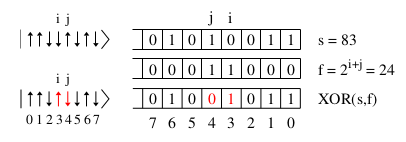
\includegraphics[scale=0.5]{fig26}
\caption{Верхняя строка показывает $N = 8$ спиновое состояние $| s \rangle$ и его представление в виде восьми первых битов целого числа $s$. Обратите внимание, что мы помечаем спины $i = 0,\dots, N - 1$ слева направо, а биты обычно обозначаются справа налево в виде двоичного числа. Чтобы перевернуть два спина $i, j$, может использоваться побитовая операция исключающее ИЛИ (XOR) с маской $f$ (средняя линия). Биты $i$ и $j$ функции $f$ устанавливаются в 1, а все остальные биты равны 0 (т. е. $f = 2^{i + j}$). В нижней строке показан результат операции XOR [ieor (s, f) в Fortran 90].}
\label{}
\end{figure}

В Фортране 90 эта операция может быть реализована как ieor $(s, 2^{ i + j})$. Позже нам также потребуются функции, выполняющие различные преобразования симметрии состояний; перевод, отражение и спин-инверсия.

Со стандартными 4-байтовыми целыми числами битовое представление с одним целым числом работает до $N = 32$. Используя длинные целые числа, можно расширить схему до $N = 64$. Последнее намного превышает максимальный размер, для которого могут применяться методы точной диагонализации. на практике, за исключением секторов намагничивания с $2m_z = n_↑ - n_↓$, достаточно большими, чтобы можно было управлять размером блока $N! / (n_↑! n_↓!)$. Намагниченность $m_z = 0$ и другие сектора с низким $m_z$ обычно представляют основной интерес.

Обсуждая алгоритмы построения базисного набора и матрицы гамильтониана, мы начнем с простейшего метода, в котором вообще не используются симметрии, а затем реализуем сохранение намагниченности. В пп. 4.1.3-4.1.5 мы включаем больше симметрий. Фактическая диагонализация матрицы гамильтониана и использование ее собственных состояний для вычисления физических наблюдаемых будет отложено до разд. 4.1.6.

\subsubsection{Компьютерная генерация гамильтониана}
Если не использовать никаких законов сохранения, гамильтониан состоит из единственной матрицы $2^N × 2^N$. Затем мы просто используем числа $a = 0, 1,\dots, 2^N - 1$ для обозначения основания состояния. Битовые значения этих целых чисел напрямую соответствуют состояниям спина. Определение $z$ диагональных вкладов $\langle a | S_i^z S_{1 + 1}^z | a \rangle = \pm 1/4$ в гамильтонову матрицу просто включает в себя проверку соответствующих битовых пар $a[i], a [i + 1]$ (одинаковых или разных), в данном случае недиагональный оператор $(S_i^{+} S_{i+1}^{-}+S_i^{-}S_{i+1}^{+}) / 2$, действующий на состояние $| a \rangle$ с $a [i] \ne a [i + 1]$, генерирует состояние $| b \rangle $, где два бита были перевернуты. Тогда матричный элемент равен $\langle b | H | a \rangle = 1/2$. Для состояния с $a[i] = a [i + 1]$, конечно, нет недиагонального матричного элемента. Следующий фрагмент псевдокода генерирует полную матрицу гамильтониана H:

\begin{lstlisting}                                {2}
do a = 0, 2^N-1
  do i = 0, N-1
    j = mod(i + 1, N)
      if (a[i] = a[ j]) then
        H(a, a) = H(a, a) + 1/4
      else
        H(a, a) = H(a, a) - 1/4
        b = flip(a, i, j); H(a, b) = 1/2
      endif
  enddo
enddo
\end{lstlisting}

Здесь j = mod (i +1, N) - «правый» ближайший сосед i, а функция mod заботится о периодической границе. В Fortran 90 проверка на a [i] = a [j] может быть реализована с помощью логической функции btest (a, i), чтобы проверить бит i из a. Каждый оператор связи в гамильтониане соответствует одному недиагональному матричному элементу, в то время как диагональные элементы имеют N различных вкладов. Матрицы, соответствующие другим интересующим операторам, конечно, могут быть построены аналогичным образом, проверяя и переворачивая биты в соответствии с любыми задействованными комбинациями операторов $S_i^z$ и $S_i^{\pm}$.

~\emph{Использование блоков с фиксированным намагничиванием.}

Двигаясь дальше в совершенстве, мы теперь реализуем сохранение намагниченности. Мы хотим построить блочный гамильтониан, действующий на все состояния с заданным $m_z = (n_↑ - n_↓) / 2$. Таких состояний $M = N! / (n_↑! n_↓!)$, И нам нужен их список. Порядок в этом списке будет использоваться как метка состояний блока, то есть мы пишем $| a\rangle$ для состояния a в списке. Затем нам также понадобится список целых чисел ( $s_a$ ), 
биты которого представляют конфигурацию вращения a  состояния. Позже нам придется выполнить поиск в списке $s_a$, чтобы найти метку позиции $a$ конкретного заданного целого числа состояния $s$, и поэтому целесообразно сделать список 
упорядоченным; $s_a < s_{a+1} $. 
Иногда мы будем использовать обозначение $| s_a \rangle $ вместо $| a \rangle$ при явном обращении к спинам, $| s_a \rangle = | s_a[0] - 1/2,\dots, s_a [N - 1] - 1 / 2 \rangle$. Из контекста будет ясно, относится ли метка внутри $| \rangle $ к позиции в списке $M$ состояний или к целому числу, содержащему спины.

Чтобы построить список состояний, мы перебираем целые числа $s = 0,\dots, 2^N - 1$ и проверяют, соответствует ли количество установленных битов (число $n_↑$ спинов ↑ в состоянии) целевому сектору; $n_↑ = m_z + N / 2$. После инициализации счетчика состояний a = 0 мы можем использовать следующий псевдокод для генерации всех состояний с заданной намагниченностью:

\begin{lstlisting}
do s = 0, 2^N-1                                    {3}
    if(sum(s[i]=n_up)) then
    	a = a + 1
	    s_a = s
    endif
enddo
M = a
\end{lstlisting}

Теперь у нас есть базис размера M, хранящийся в виде целых чисел $s_a, a = 1,\dots , М$.

Чтобы построить гамильтониан, мы перебираем метки $a = 1, \dots, M$ и используем битовые операции, как и раньше, для воздействия на соответствующие целые числа состояния $s_a$. Когда недиагональная операция над $| s_a \rangle$ приводит к другому состоянию $| s^{∗} = | s_b \rangle$, и необходимо найти позицию $b$ целого числа $s^{∗}$ в списке состояний. Поскольку этот список упорядочен, мы можем сделать это путем поиска пополам за $\sim log_2(M)$ шагов в среднем. Такой поиск проходит через серию векторов, где на каждом шаге мы можем вдвое сократить возможный диапазон $b$, исследуя состояние в средней точке диапазона $[b_min, b_max]$, с скобками $b_min = 1$ и $b_max = M$ изначально. Следующая подпрограмма находит позицию $b$ целого числа $s^∗$;

\begin{lstlisting}
subroutine findstate(s*,b)                         {4}
  b min = 1; 
  b max = M
  do
    b = b_min + (b_max - b_min )/2
    if (s* < s_b) then
      b_max = b-1
    elseif (s*>s_b) then
      b_min = b + 1
    else
      exit
    endif
enddo
\end{lstlisting}

Деление целого числа на 2 здесь следует рассматривать стандартным образом, т.е. $i / 2$ для нечетного $i$ равно $(i - 1) / 2$. Выход из цикла происходит, когда базовое состояние $s_b$ равно целевому состоянию $s^∗$. Можно также использовать более эффективные поисковые процедуры с использованием так называемых хеш-таблиц [145]. Однако деление пополам намного проще и в большинстве случаев достаточно быстро.

Используя подпрограмму (4), часть гамильтониана, возникающая в результате операции со спиновой парой $(i, j)$ в состоянии $| a \rangle$, может быть построена с помощью следующей модификации кода {2};

\begin{lstlisting}
if (s_a[i] = s_a[j]) then                        {5}
  H(a, a) = H(a, a) + 1/4
else
  H(a, a) = H(a, a) - 1/4
  s*=flip(s_a,i,j)
  call findstate(s*, b)
  H(a, b) = 1/2
endif
\end{lstlisting}

Если кто-то просто заинтересован в получении быстрых результатов для какой-то очень маленькой решетки или если система не является периодической (открытая цепочка или система со случайными связями, и в этом случае импульс не сохраняется), может быть достаточно построить гамильтониан в таком виде и приступить к его диагонализации (последовательно для всех желаемых $m_z$ -блоков). Для серьезной работы над трансляционно-инвариантными (периодическими) системами стоит реализовать дополнительные симметрии для дальнейшей блочной диагонализации фиксированных $m_z$ блоков.

\subsubsection{Состояния моментов}
Теперь мы построим собственные состояния оператора сдвига $T$, определенного уравнением. (~\ref{eq_107}). Выполнение $N$ шагов возвращает вращения в исходное состояние. Таким образом, $T^N = 1$, что означает собственные значения $e^{ik}$, где набор из $N$ неэквивалентных импульсов может быть выбран как

\begin{equation}
k=m\frac{2\pi}{N}, m = -N/2+1,\dots,N/2
\label{eq_114}
\end{equation}

с постоянной решетки, равной 1. Состояние импульса может быть построено с использованием эталонного состояния $| a \rangle $ (единственное состояние в базисе z-компоненты) и всех его трансляций;

\begin{equation}
|a(k)\rangle=\frac{1}{\sqrt{N_a}}\sum\limits_{r=0}^{N-1}e^{-ikr}T^r|a \rangle
\label{eq_115}
\end{equation}

Легко проверить (с помощью сдвига индекса суммирования, допустимого из-за периодических границ), что работа с оператором сдвига (~\ref{eq_107}) в этом состоянии дает $T | a (k) \rangle = e^{ik} | a (k) \rangle$, что является определением импульсного состояния.

Чтобы построить базис момента для данного k (и, как правило, также для данного $m^z$), мы должны найти набор представителей, приводящих к полному набору нормализуемых ортогональных состояний. Ясно, что для того, чтобы два состояния $| a (k) \rangle$ и $| b (k) \rangle$ были ортогональными, соответствующие представители должны подчиняться $T^r | a\rangle = | b \rangle$ для всех $r$. Следовательно, среди всех состояний множества транслированных состояний $| a(r) \rangle = T^r | a \rangle, r = 0,\dots , N - 1$, в качестве представителя следует использовать только один. С метками, относящимися к битовому представлению, будет практично всегда выбирать представителя как тот, для которого целое число $a(r)$ является наименьшим (как определено путем выполнения всех преобразований).

\subsubsection{Точная диагонализация цепи Гейзенберга S = 1/2 без использования симметрии}

Исходный код программы приведен в Приложении 1\\

Результат работы алгоритма выводится в виде матрицы, где: \\
\begin{tabular}{llll}
Столбец 1 & Номер собственного значения; 0, ..., 2 N -1 \\
Столбец 2 & собственное значение энергии \\
Столбец 3 & ожидаемое значение полного спина S; извлечено из $<S⋅S> = S (S + 1)$ \\
Столбец 4 & ожидаемое значение намагниченности (ось z)\\
\end{tabular} \\

Периодические граничные условия для N = 2:\\
\begin{tabular}{llll}
    0 & -1,5000000000 & 0,0000000000 & -0,0000000000 \\
    1 & 0.5000000000 & 1.0000000000 & -0.5000000000 \\
    2 & 0.5000000000 & 1.0000000000 & -0.0000000000 \\ 
    3 & 0.5000000000 & 1.0000000000 & 0.5000000000 \\
\end{tabular}\\

Для N = 4 были получены результаты.  \\
\begin{tabular}{llll}
    0 & -2,0000000000 & 0,0000000000 & 0,0000000000 \\
    1 & -1.0000000000 & 1.0000000000 & -0.5000000000 \\
    2 & -1.0000000000 & 1.0000000000 & 0.0000000000 \\
    3 & -1.0000000000 & 1.0000000000 & 0.5000000000 \\
    4 & -0.0000000000 & 1.0000000000 & -0.5000000000 \\
    5 & -0.0000000000 & 1.0000000000 & 0.5000000000 \\
    6 & 0,0000000000 & 0,5029870708 & -0,0000000000 \\
    7 & 0,0000000000 & 0,9699263936 & -0,0000000000 \\
    8 & 0,0000000000 & 0,7583057392 & 0,0000000000 \\
    9 & 0.0000000000 & 1.0000000000 & 0.5000000000 \\
   10 & 0.0000000000 & 1.0000000000 & -0.5000000000 \\
   11 & 1.0000000000 & 2.0000000000 & -0.5000000000 \\
   12 & 1.0000000000 & 2.0000000000 & -1.0000000000 \\
   13 & 1.0000000000 & 2.0000000000 & 0.5000000000 \\
   14 & 1.0000000000 & 2.0000000000 & 0.0000000000 \\
   15 & 1.0000000000 & 2.0000000000 & 1.0000000000 \\
\end{tabular} \\

Обратите внимание, что состояния 6-8 вырождены (те же энергии в столбце 2) с одинаковой намагниченностью z (столбец 4). Общий спин (столбец 3) не диагональный, так как нецелые математические ожидания не соответствуют разрешенным S собственным значениям. Линейная комбинация 3 вырожденных состояний с различными S была произведена процедурой диагонализации.\\

Для N = 8 приведены 16 первых собственных значений: \\
\begin{tabular}{llll}
    0 & -3,6510934089 & 0,0000000000 & 0,0000000000 \\
    1 & -3.1284190638 & 1.0000000000 & -0.4999786387 \\
    2 & -3.1284190638 & 1.0000000000 & -0.0000213613 \\
    3 & -3.1284190638 & 1.0000000000 & 0.5000000000 \\
    4 & -2,6996281483 & 0,0000000000 & 0,0000000000 \\
    5 & -2,4587385089 & 1,000000000000 & -0,4482606137 \\
    6 & -2.4587385089 & 1.0000000000 & 0.4999793383 \\
    7 & -2,4587385089 & 1,000000000000 & -0,0427976061 \\
    8 & -2,4587385089 & 1,000000000000 & 0,0059285074 \\
    9 & -2,4587385089 & 1,000000000000 & -0,4725423843 \\
   10 & -2,4587385089 & 1,000000000000 & 0,4576927583 \\
   11 & -2,1451483739 & 1,0000000000 & -0,4622747971 \\
   12 & -2,1451483739 & 1,000000000000 & 0,3924081181 \\
   13 & -2,1451483739 & 1,000000000000 & -0,1595269579 \\
   14 & -2.1451483739 & 1.0000000000 & 0.4890986185 \\
   15 & -2,1451483739 & 1,000000000000 & -0,1851207824 \\
\end{tabular} \\

 Обратите внимание на множество вырожденных состояний с h идентичным спином (столбец 2) и тот факт, что теперь значения z-намагниченности (столбец 4), как правило, не являются допустимыми собственными значениями намагниченности. Это связано с тем, что подпрограмма диагонализации (в зависимости от того, как именно она работает) может смешивать состояния с одинаковыми E, S и разной намагниченностью, если матрица гамильтониана не записана в блочно-диагональной форме намагниченности.

\subsubsection{Точная диагонализация цепи Гейзенберга S = 1/2 с сохранением намагниченности}
Листинг программы приведен в Приложение 2.

Для каждого сектора фиксированного числа вращений вверх $\nu$:\\
\begin{tabular}{ll}
Столбец 1 & $\nu$  \\
Столбец 2 & размер блока nst \\
Столбец 3 & Номер собственного значения (целое число) \\
Столбец 4 & Собственное значение энергии (действительное ) \\
Столбец 5 & Спиновое квантовое число (действительное). \\
\end{tabular}\\

Периодические граничные условия используются также для N = 2, в результате чего энергии вдвое превышают нормальные синглетные / триплетные энергии: \\

\begin{tabular}{lllll}
 0 & 1 & 0 & 0,5000000000 & 1,000000000000 \\
 1 & 2 & 0 & -1,5000000000 & 0,0000000000 \\
 1 & 2 & 1 & 0.5000000000 & 1.0000000000 \\
\end{tabular}

Ниже приведены результаты для N = 4. Обратите внимание, что состояния 2–4 для $\nu$ = 2 являются вырожденными (те же энергии в столбце 2). В этом случае общее вращение (столбец 3) не диагонально. Некоторые линейные комбинации трех вырожденных состояний производятся процедурой диагонализации, в результате чего вычисленное математическое ожидание полного спина не является собственными значениями:\\

\begin{tabular}{lllll}
    0 & 1 & 0 & 1,0000000000 & 2,0000000000 \\
    1 & 4 & 0 & -1,0000000000 & 1,0000000000 \\
    1 & 4 & 1 & -0,0000000000 & 1,0000000000 \\
    1 & 4 & 2 & 0,0000000000 & 1,000000000000 \\
    1 & 4 & 3 & 1,0000000000 & 2,0000000000 \\
    2 & 6 & 0 & -2,0000000000 & 0,0000000000 \\
    2 & 6 & 1 & -1,0000000000 & 1,0000000000 \\
    2 & 6 & 2 & 0,0000000000 & 0,5029870708 \\
    2 & 6 & 3 & 0,0000000000 & 0,9699263936 \\
    2 & 6 & 4 & 0,0000000000 & 0,7583057392 \\
    2 & 6 & 5 & 1,0000000000 & 2,0000000000 \\
\end{tabular} \\

Это самая низкая пара собственных значений для mz = 0, ..., 6 секторов 12-узловой цепочки: \\
\begin{tabular}{lllll}
    0 & 1 & 0 & 3,0000000000 & 6,0000000000 \\
    1 & 12 & 0 & 1,0000000000 & 5,0000000000 \\
    1 & 12 & 1 & 1,1339745962 & 5,0000000000 \\
    2 & 66 & 0 & -0,9189859472 & 4,0000000000 \\
    2 & 66 & 1 & -0,6609656356 & 4,0000000000 \\
    3 & 220 & 0 & -2,6517399155 & 3,0000000000 \\
    3 & 220 & 1 & -2,2903940178 & 3,0000000000 \\
    4 & 495 & 0 & -4,0705293260 & 2,0000000000 \\
    4 & 495 & 1     & -3,6374064252      & 2,0000000000 \\
    5 & 792 &  0     & -5,0315434037      & 1,0000000000 \\
    5 & 792 &  1     & -4,5693744108      & 1,0000000000 \\
    6 & 924 &  0     & -5,3873909174      & 0,0000000000 \\
	6 & 924 &  1     & -5,0315434037      & 1,0000000000 \\
\end{tabular} \\

Здесь самый большой размер матрицы уже составляет 924 * 924, и, таким образом, не намного большие размеры системы могут быть обработаны без использования дополнительных симметрий для дальнейшей диагонализации блоков.

\subsubsection{Точная диагонализация цепи Гейзенберга S = 1/2 с использованием импульсных состояний.}

Листинг кода приведен в Приложении 3 \\

Для каждого сектора с фиксированным числом вращений вверх $\nu$ и импульсом k (целое число, k = 0, ..., N / 2) файл eig.dat:: \\
\begin{tabular}{ll}
Столбец 1 & $\nu$ \\
Столбец 2 & k \\
Столбец 3 & nst \\
Столбец 4 & Число собственных значений (целое число) \\
Столбец 5 & Собственное значение энергии (действительное) \\
Столбец 6 & Квантовое число спина (действительное) \\
\end{tabular}

Ниже приведены результаты для N = 6 \\
\begin{tabular}{llllll}
 0 & 0 & 1 & 0 & 1.5000000000 & 3.0000000000 \\
 1 & 0 & 1 & 0 & 1.5000000000 & 3.0000000000 \\
 1 & 1 & 1 & 0 & 1.0000000000 & 2.0000000000 \\
 1 & 2 & 1 & 0 & -0.0000000000 & 2.0000000000 \\
 1 & 3 & 1 & 0 & -0.5000000000 & 2.0000000000 \\
 2 & 0 & 3 & 0 & -2,1180339887 & 1,000000000000 \\
 2 & 0 & 3 & 1 & 0.1180339887 & 1.0000000000 \\
 2 & 0 & 3 & 2 & 1.5000000000 & 3.0000000000 \\
 2 & 1 & 2 & 0 & -1.0000000000 & 1.0000000000 \\
 2 & 1 & 2 & 1 & 1.0000000000 & 2.0000000000 \\
 2 & 2 & 3 & 0 & -1.2807764064 & 1.0000000000 \\
 2 & 2 & 3 & 1 & 0,0000000000 & 2,000000000000 \\
 2 & 2 & 3 & 2 & 0,7807764064 & 1,000000000000 \\
 2 & 3 & 2 & 0 & -0.5000000000 & 2.0000000000 \\
 2 & 3 & 2 & 1 & 0.5000000000 & 1.0000000000 \\
 3 & 0 & 4 & 0 & -2,1180339887 & 1,000000000000 \\
 3 & 0 & 4 & 1 & -1,5000000000 & 0,0000000000 \\
 3 & 0 & 4 & 2 & 0.1180339887 & 1.0000000000 \\
 3 & 0 & 4 & 3 & 1.5000000000 & 3.0000000000 \\
 3 & 1 & 3 & 0 & -1.0000000000 & 1.0000000000 \\
 3 & 1 & 3 & 1 & -0,5000000000 & 0,0000000000 \\
 3 & 1 & 3 & 2 & 1.0000000000 & 2.0000000000 \\
 3 & 2 & 3 & 0 & -1.2807764064 & 1.0000000000 \\
 3 & 2 & 3 & 1 & -0.0000000000 & 2.0000000000 \\
 3 & 2 & 3 & 2 & 0,7807764064 & 1,000000000000 \\
 3 & 3 & 4 & 0 & -2,8027756377 & 0,0000000000 \\
 3 & 3 & 4 & 1 & -0.5000000000 & 2.0000000000 \\
 3 & 3 & 4 & 2 & 0.5000000000 & 1.0000000000 \\
 3 & 3 & 4 & 3 & 0.8027756377 & 0.0000000000 \\

\end{tabular}


Результат, содержащий наименьшее собственное состояние для каждого сектора:\\
\begin{tabular}{ll}
Столбец 1 & k (целое число)\\
Столбец 4 & Собственное значение энергии (действительное)\\
Столбец 5 & Квантовое число спина (действительное)\\
\end{tabular} \\

\begin{tabular}{lllll}
    0 & 0 & 1.5000000000 & 3.0000000000 & 1 \\
    1 & 0 & 1.5000000000 & 3.0000000000 & 1 \\
    1 & 1 & 1.0000000000 & 2.0000000000 & 1 \\
    1 & 2 & -0.0000000000 & 2.0000000000 & 1 \\
    1 & 3 & -0.5000000000 & 2.0000000000 & 1 \\
    2 & 0 & -2,1180339887 & 1,000000000000 & 3 \\
    2 & 1 & -1.0000000000 & 1.0000000000 & 2 \\
    2 & 2 & -1.2807764064 & 1.0000000000 & 3 \\
    2 & 3 & -0.5000000000 & 2.0000000000 & 2 \\
    3 & 0 & -2,1180339887 & 1,000000000000 & 4 \\
    3 & 1 & -1.0000000000 & 1.0000000000 & 3 \\
    3 & 2 & -1.2807764064 & 1.0000000000 & 3 \\
    3 & 3 & -2,8027756377 & 0,0000000000 & 4 \\
\end{tabular}\\

При N = 6 все (mz, k) состояния имеют фиксированный суммарный спин, как можно видеть из целочисленных значений, полученных для S. При больших N все еще существуют некоторые случаи вырождения состояний с разными S. N = 8, есть такой случай 3 вырожденных состояний с $\nu$ = 2, k = 4, как видно из рассчетов для этого сектора:\\

\begin{tabular}{llllll}
    2 & 4 & 4 & 0 & -0,0000000000 & 2,0009877794 \\
    2 & 4 & 4 & 1 & 0,0000000000 & 2,9990995860 \\
    2 & 4 & 4 & 2 & 0,0000000000 & 2,0002724281 \\
    2 & 4 & 4 & 3 & 1.0000000000 & 2.0000000000 \\
\end{tabular}

\subsubsection{ Точная диагонализация цепочки Гейзенберга S = 1/2 с использованием полуимпульсных состояний}

Листинг кода программы приведен в Приложение 4. \\

За исключением k = 0 и k = pi (целочисленная метка k = N / 2), симметричные (p = 1) и антисимметричные (p = -1) состояния являются вырожденными (так же, как состояния с регулярным импульсом с импульсом k и -k вырождены). Таким образом, программа выполняет расчет для p = -1 и p = + 1 только для k = 0 и pi, и только для p = + 1 для других импульсов.

Для каждого сектора с фиксированным количеством вращений вверх nu и импульсом k (целое число, k = 0, ..., N / 2) и p (-1 и +1):


\begin{tabular}{ll}
Столбец 1 & $\nu$ \\
Столбец 2 & k \\ 
Столбец 3 & p \\
Столбец 4 & размер блока nst\\
Столбец 5 & Число собственных значений (целое число)\\
Столбец 6 & Собственное значение энергии (действительное)\\
Столбец 7 & Квантовое число спина (действительное)\\
\end{tabular}\\

Ниже приведены результаты для N = 6. Обратите внимание, что для этой небольшой системы многие секторы не имеют состояний:\\

\begin{tabular}{lllllll}
	nu = 0 & k = 0 & p = -1 & nst = 0& & & \\
	nu = 0 & k = 0 & p = 1 & nst = 1& & &\\
	& & & & 0 & 0,0000000000 & 3,000000000000\\
\end{tabular}

\begin{tabular}{lllllll}
	nu = 0 & k = 1 & p = 1 & nst = 0 & & & \\
	nu = 0 & k = 2 & p = 1 & nst = 0 & & & \\
	nu = 0 & k = 3 & p = -1 & nst = 0 & & & \\
	nu = 0 & k = 3 & p = 1 & nst = 0 & & &  \\
	nu = 1 & k = 0 & p = -1 & nst = 0 & & & \\
	nu = 1 & k = 0 & p = 1 & nst = 1 & & & \\
	& & & & 0 & 0,0000000000 & 3,000000000000 \\
\end{tabular}

\begin{tabular}{lllllll}	
	nu = 1 & k = 1 & p = 1 & nst = 1 & & & \\
    & & & & 0 & 0,0000000000 & 2,000000000000 \\
\end{tabular}

\begin{tabular}{lllllll}
nu = 1 & k = 2 & p = 1 & nst = 1 & & & \\
    & & & & 0 & 0,0000000000 & 2,000000000000 \\
\end{tabular}

\begin{tabular}{lllllll}    
nu = 1 & k = 3 & p = -1 & nst = 1 & & & \\
    & & & & 0 & 0,0000000000 & 2,000000000000 \\
\end{tabular}

\begin{tabular}{lllllll}    
nu = 1 & k = 3 & p = 1 & nst = 0 & & & \\
nu = 2 & k = 0 & p = -1 & nst = 0 & & & \\
nu = 2 & k = 0 & p = 1 & nst = 3 & & & \\
    & & & & 0 & -2,1180339887 & 1,000000000000 \\
    & & & & 1 & 0.1180339887 & 1.0000000000 \\
    & & & & 2 & 0.0000000000 & 3.0000000000 \\
\end{tabular}

\begin{tabular}{lllllll}    
nu = 2 & k = 1 & p = 1 & nst = 2 & & & \\
    & & & & 0 & -1.0000000000 & 1.0000000000 \\
    & & & & 1 & 1.0000000000 & 2.0000000000 \\
\end{tabular}

\begin{tabular}{lllllll}    
nu = 2 & k = 2 & p = 1 & nst = 3 & & & \\
    & & & & 0 & -1.2807764064 & 1.0000000000\\
    & & & & 1 & 0,0000000000 & 2,000000000000\\
    & & & & 2 & 0,0000000000 & 1,000000000000 \\
\end{tabular}

\begin{tabular}{lllllll}    
nu = 2 & k = 3 & p = -1 & nst = 1 & & & \\
    & & & & 0 & 0,0000000000 & 2,000000000000 \\
nu = 2 & k = 3 & p = 1 & nst = 1 & & & \\
    & & & & 0 & 0,0000000000 & 1,000000000000 \\
nu = 3 & k = 0 & p = -1 & nst = 1 & & & \\
    & & & & 0 & 0,0000000000 & 0,0000000000 \\
nu = 3 & k = 0 & p = 1 & nst = 3 & & & \\
    & & & & 0 & -2,1180339887 & 1,000000000000 \\
    & & & & 1 & 0.1180339887 & 1.0000000000 \\
    & & & & 2 & 0.0000000000 & 3.0000000000 \\
\end{tabular}

\begin{tabular}{lllllll}    
nu = 3 & k = 1 & p = 1 & nst = 3 & & & \\
    & & & & 0 & -1.0000000000 & 1.0000000000\\
    & & & & 1 & -0,5000000000 & 0,0000000000\\
    & & & & 2 & 0,0000000000 & 2,000000000000\\
\end{tabular}

\begin{tabular}{lllllll}    
nu = 3 & k = 2 & p = 1 & nst = 3 & & & \\
    & & & & 0 & -1.2807764064 & 1.0000000000\\
    & & & & 1 & -0.0000000000 & 2.0000000000 \\
    & & & & 2 & 0,0000000000 & 1,000000000000\\
\end{tabular}

\begin{tabular}{lllllll}    
nu = 3 & k = 3 & p = -1 & nst = 3 & & & \\
    & & & & 0 & -2,8027756377 & 0,0000000000\\
    & & & & 1 & -0.5000000000 & 2.0000000000\\
    & & & & 2 & 0,0000000000 & 0,0000000000\\
\end{tabular}

\begin{tabular}{lllllll}    
nu = 3 & k = 3 & p = 1 & nst = 1 & & & \\
    & & & & 0 & 0,0000000000 & 1,000000000000 \\
\end{tabular}\\


Файл с результатами рассчетов, содержащий наименьшее собственное состояние для каждого сектора: \\

\begin{tabular}{ll}
Столбец 1 & nu (целое число) \\
Столбец 2 & k (целое число) \\
Столбец 3 & p (целое число) \\
Столбец 4 & Собственное значение энергии (действительное) \\
Столбец 5 & Квантовое число спина (действительное) \\
\end{tabular}\\

Рассчетные значения: \\

\begin{tabular}{llllll}
    0 & 0 & 1 & 0.0000000000 & 3.0000000000 & 1 \\
    1 & 0 & 1 & 0.0000000000 & 3.0000000000 & 1 \\
    1 & 1 & 1 & 0.0000000000 & 2.0000000000 & 1 \\
    1 & 2 & 1 & 0.0000000000 & 2.0000000000 & 1 \\
    1 & 3 & -1 & 0,0000000000 & 2,0000000000 & 1 \\
    2 & 0 & 1 & -2,1180339887 & 1,000000000000 & 3 \\
    2 & 1 & 1 & -1.0000000000 & 1.0000000000 & 2 \\
    2 & 2 & 1 & -1.2807764064 & 1.0000000000 & 3 \\
    2 & 3 & -1 & 0,0000000000 & 2,0000000000 & 1 \\
    2 & 3 & 1 & 0.0000000000 & 1.0000000000 & 1 \\
    3 & 0 & -1 & 0,0000000000 & 0,0000000000 & 1 \\
    3 & 0 & 1 & -2,1180339887 & 1,000000000000 & 3 \\
    3 & 1 & 1 &  -1.0000000000 & 1.0000000000 & 3 \\
    3 & 2 & 1 & -1.2807764064 & 1.0000000000 & 3 \\
    3 & 3 & -1 & -2,8027756377 & 0,0000000000 & 3 \\
    3 & 3 & 1 & 0.0000000000 & 1.0000000000 & 1 \\
\end{tabular}\\

Интересно посмотреть на состояния с nu = 2 и k = pi для N = 8. Когда четность не используется, есть 3 вырожденных состояния с энергией E = 0 и различным полным спином, диагонализация дает нецелое число S \\

\begin{tabular}{llllll}
 	nu = 2 & k = 4 & nst = 4 & & & \\
    & & & 0 & -0,0000000000 & 2,0009877794 \\
    & & & 1 & 0,0000000000 & 2,9990995860 \\
    & & & 2 & 0,0000000000 & 2,0002724281 \\
    & & & 3 & 1.0000000000 & 2.0000000000 \\
\end{tabular}\\

При использовании паритета часть этого вырождения снимается. Состояния в секторах p = -1 и p = + 1 равны:\\

\begin{tabular}{lllllll}
	nu = 2 & k = 4 & p = -1 & nst = 2 & & & \\
    & & & 0 & 0,0000000000 & 2,7015621187 \\
    & & & 1 & 0,0000000000 & 2,3722813233 \\
	nu = 2 & k = 4 & p = 1 & nst = 2 & & & \\
    & & & 0 & 0,0000000000 & 2,000000000000 \\
    & & & 1 & 1.0000000000 & 2.0000000000 \\
\end{tabular}\\
    
    В секторе p = + 1 имеется одно состояние с E = 0, со спином S = 2. В секторе p = -1 все еще есть 2 вырожденных состояния с разными спинами, которые не разрешаются этой диагонализацией (хотя на основе полученной информации мы все еще можем в принципе вычислить спины, поскольку только одно конкретное смешивание двух целочисленных спинов может дать ожидаемые значения, предоставленные программой).
    
\subsection{Метод Ланцоша}
Как мы видели в предыдущем разделе, полная диагонализация гамильтониана (или отдельных блоков) становится чрезмерно трудоемкой для систем S = 1/2 с более чем $\approx 20$ спинов. Для более высоких S ситуация, конечно, еще хуже. Если мы ограничимся только основным состоянием и, возможно, рядом низколежащих возбуждений, мы сможем достичь систем примерно в два раза больше, используя технику пространства Крылова, такую как метод Ланцоша.

\subsubsection{Пространство Крылова}
Пространство Крылова - это подпространство полного гильбертова пространства, построенное таким образом, что низколежащие состояния интересующего гамильтониана H должны быть хорошо аппроксимированы в нем. Рассмотрим произвольное состояние 
$|\psi \rangle$, например, состояние со случайно сгенерированными векторными элементами $\psi(i), i = 1,\dots, M$, в M-мерном гильбертовом пространстве, в котором определен H, и разложение этого состояния по собственным гамильтоновым состояниям $|\psi_n \rangle$ (в порядке возрастания собственных значений, которые мы здесь обозначили $n = 0, 1, \dots , M - 1$). Мы работаем со степенью гамильтониана на этом выбранном состоянии;

\begin{equation}
H^{\Lambda}|\psi \rangle = \sum_{n=0}^{M-1}c_nE_n^{\Lambda}|\psi_n\rangle = c_{max}E_{max}^{\Lambda}[|\psi_max \rangle + \sum\limits_{n \ne max} \frac{c_n}{c_max}(\frac{E_n}{E_max})^{\Lambda}|\psi_n\rangle]
\label{eq_170}
\end{equation}

Если мощность $\Lambda$ велика, состояние, соответствующее собственному значению $| E_ max |$ с наибольшей величиной (т. е. $max = 0$ или $max = M - 1$) будет преобладать над суммой при условии, что коэффициент расширения $c_max \ne 0$. Следовательно, многократное воздействие гамильтонианом на состояние будет проецировать собственный вектор с собственное значение $E_max$. 
Если мы хотим убедиться, что основное состояние $|\psi_0 \rangle$ (точно при $\Lambda \to \infty$ или приближенно для конечного $\Lambda$), мы можем вместо $H^{\Lambda}$ использовать $(H-c)^\Lambda$, где $c$ - достаточно большое положительное число, чтобы гарантировать, что $| E_0 - c | > | E_{M − 1} - с |$. Здесь мы будем предполагать, что такая постоянная, если потребуется, уже поглощена H.

Хотя уравнение ~\ref{eq_170} гарантированно создает основное состояние, когда $\Lambda$ достаточно велико, более эффективный способ построить состояние, которое приближается к основному состоянию при $\Lambda \to \infty$, - это рассматривать не только $H^{\Lambda}|\psi \rangle$, но и все подпространство гильбертова пространство, натянутое на множество состояний $H^m |\psi \rangle, m = 0,\dots, \Lambda$. Эти состояния могут быть построены одно за другим путем последовательных операций с $H$ над начальным состоянием $| \psi\rangle $. В этом подпространстве существует оптимальная линейная комбинация векторов, аппроксимирующая основное состояние (минимизирующая ожидаемое значение энергии), и способ найти ее - диагонализовать $H$ в
 сгенерированном подпространстве $\Lambda + 1$ векторов. В дополнение к проецированию основного состояния для относительно малых $\Lambda$ (часто на много порядков меньше, чем размер $M$ полного гильбертова пространства), этот подход также может точно воспроизвести ряд низколежащих возбужденных состояний. Подпространство гильбертова пространства, полученное многократным воздействием с $H$ на начальное состояние, называется пространством Крылова. Здесь мы обсуждаем гамильтонианы в квантовой механике, но методы пространства Крылова, конечно, применимы и к задачам на собственные значения в более общем плане, и очень широко используются во многих областях науки и техники.

\subsubsection{Базис Ланцоша и гамильтониан}
В методе Ланцоша [148] ортогональный базис строится с использованием линейных комбинаций состояний пространства Крылова, так что гамильтониан, записанный в этом базисе, является трехдиагональным. В стандартном подходе, который будет описан ниже, в основе ${| f_m \rangle}, m = 0,\dots , \Lambda$, сначала строится ортогонально, но не нормировано. Эти состояния впоследствии будут нормализованы, чтобы получить ортонормированный набор {$| \phi_m \rangle$}, в котором гамильтониан принимает особенно простой трехдиагональный вид. Мы также обсудим несколько иной подход к непосредственной генерации нормализованного базиса {$| \phi_m \rangle$}.

~\emph{Генерация базиса Ланцоша}
Построение основы {$| f_m \rangle$} начинается с произвольного нормализованного состояния | $f_0 \rangle$, от которого требуется только, чтобы он не был ортогонален основному состоянию H (если цель состоит в том, чтобы найти основное состояние). Так должно быть для случайно сгенерированного $| f_0 \rangle $, но можно также начать с некоторого вектора, который, как известно, имеет существенное перекрытие с основным состоянием. Следующее состояние задается

\begin{equation}
|f_1\rangle = H|f_0\rangle-a_0|f_0\rangle
\label{eq_171}
\end{equation}

где постоянную $a_0$ следует определить так, чтобы $| f_1 \rangle$ ортогонален $| f_0 \rangle$. С этой целью мы исследуем совпадение двух состояний;

\begin{equation}
\langle f_1 | f_0 \rangle = \langle f_0 | H | f_0 \rangle - a_0 \langle f_0 | f_0 \rangle = H_{00} - a_0 N_0
\label{eq_172}
\end{equation}

де мы ввели обозначения для нормировочных констант и диагональных матричных элементов гамильтониана, которые также будут использоваться для последующих состояний;

\begin{equation}
N_m = \langle f_m | f_m \rangle
\label{eq_173}
\end{equation}

\begin{equation*}
H_{mm} = \langle f_m |H| f_m \rangle
\end{equation*}

Чтобы перекрытие (~\ref{eq_172}) исчезло, мы должны выбрать $a_0 = H_{00} / N_0$. Следующее состояние m = 2 записывается в терминах двух предыдущих как

\begin{equation}
|f_2 \rangle = H |f_1 \rangle - a_1|f_1 \rangle - b_0|f_0 \rangle
\label{eq_174}
\end{equation}

где $a_1$ и $b_0$ можно выбрать так, чтобы $| f_2 \rangle$ ортогонален обоим $| f_0 \rangle$ и $| f_1 \rangle$. Перекрытия при использовании $H | f_0 \rangle и H | f_1 \rangle$, полученный из уравнений (~\ref{eq_171}) и (~\ref{eq_174});

\begin{equation}
\langle f_2 | f_1 \rangle = H_{11} - a_1N_1
\label{eq_175}
\end{equation}

\begin{equation*}
\langle f_2 | f_0 \rangle = N_1-b_0N_0
\end{equation*}

Таким образом, подходящими коэффициентами являются $a_1 = H_{11} / N_1$ и $b 0 = N_1 / N_0$. Для всех последующих итераций уравнение. (~\ref{eq_174}) обобщается на

\begin{equation}
| f_{m+1} \rangle = H |f_m \rangle - a_m|f_m \rangle - b_{m-1}|f_{m-1} \rangle
\label{eq_176}
\end{equation}

и коэффициенты, делающие это состояние ортогональным $| f_m \rangle$ и $| f_{m − 1}  \rangle $ являются обобщениями уже найденных нами выражений для $a_0$, $a_1$ и $b_0$;

\begin{equation}
a_m = H_{mm}/N_m
\label{eq_177}
\end{equation}

\begin{equation*}
b_{m-1} = N_m/N_{m-1}
\end{equation*}

Это легко проверить прямым вычислением перекрытий. Остается показать, что с этими коэффициентами состояние $| f_{m + 1} \rangle$ ортогонален также всем предыдущим состояниям $| f_k \rangle $ при $k <m - 1$. В индуктивном доказательстве мы можем использовать

\begin{equation*}
\langle f_{m+1}|f_{m-k}\rangle = \langle f_m | H | f_{m-k} \rangle 
- a_m \langle f_m | f_{m-k} \rangle
- b_{m-1} \langle f_{m-1} | f_{m-k} \rangle 
\end{equation*}

\begin{equation}
= \langle f_m | f_{m-k+1} \rangle
+ a_{m-k} \langle f_m | f_{m-k} \rangle
+ b_{m-k+1} \langle f_{m} | f_{m-k-1} \rangle = 0
\label{eq_178}
\end{equation}

где мы также использовали $H | f_{m − k} \rangle$ в форме, заданной формулой. (~\ref{eq_176}).

Эта итерационная процедура (~\ref{eq_176}) продолжается до тех пор, пока $m = \Lambda$, где $\Lambda$ может быть определено автоматически, на лету, в соответствии с некоторым критерием сходимости для вычисленных величин, как мы обсудим ниже. Сначала нам понадобятся матричные элементы гамильтониана.

~\emph{Гамильтониан в базисе Ланцоша}
Построив набор из $\Lambda + 1$ векторов Ланцоша $| f_m \rangle, m = 0,\dots , \Lambda $, гамильтониан в этом базисе может быть построен. Мы можем использовать выражение для $H$, действующего на одно из базисных состояний, полученное из уравнения. (~\ref{eq_176});


\begin{equation}
H|f_m \rangle = |f_{m+1} \rangle + a_m |f_m \rangle + b_{m-1} |f_{m-1} \rangle
\label{eq_179}
\end{equation}

и, таким образом, ненулевые матричные элементы равны

\begin{equation*}
\langle f_{m-1}|H|f_m\rangle = b_{m-1}N_{m-1} = N_m
\end{equation*}

\begin{equation}
\langle f_m|H|f_m\rangle = a_m N_m
\label{eq_180}
\end{equation}

\begin{equation*}
\langle f_{m+1}|H|f_m\rangle = N_{m+1}
\end{equation*}

Нормализованные базисные состояния:

\begin{equation}
\langle |\phi_m \rangle = \frac{1}{\sqrt{N_m}}|f_m \rangle
\label{eq_181}
\end{equation}

и $b_m = N_{m + 1} / N_m$ согласно (~\ref{eq_177}). Следовательно, ненулевые элементы матрицы

\begin{equation*}
\langle \phi_{m-1}|H|\phi_m\rangle = \sqrt{b_m-1}
\end{equation*}


\begin{equation}
\langle \phi_m|H|\phi_m\rangle = a_m
\label{eq_186}
\end{equation}

\begin{equation*}
\langle \phi_{m+1}|H|\phi_m\rangle = \sqrt{b_m}
\end{equation*}

Это трехдиагональная матрица, которую можно диагонализовать с помощью специальных методов, которые быстрее обычных алгоритмов диагонализации (доступны во многих библиотеках подпрограмм линейной алгебры). Однако главное преимущество состоит не в том, что матрицу легче диагонализовать - она в любом случае обычно не очень велика, и даже если используется обычная процедура диагонализации, время, затрачиваемое на эту часть вычислений, незначительно. Преимущество состоит в том, что эта матрица может быть построена относительно быстро, особенно когда матрица H разреженная и должны учитываться только ее ненулевые элементы (сохраняются или генерируются на лету при воздействии H на состояние). Иногда, когда метод применяется к очень большим матрицам, также полезно, чтобы только три больших вектора состояния $| f_m \rangle $ должен быть сохранен в процессе. Трехдиагональность также очень удобна при вычислении спектральных функций (динамических корреляций), как это обсуждается, например, в работах [43, 143].//

~\emph{Вырожденные состояния}
Следует отметить, что метод Ланцоша не может дать больше чем один член мультиплета; из вырожденного множества состояний будет получена только конкретная их линейная комбинация (которая зависит от начального состояния $| f_0 \rangle$).
 Чтобы понять причину этого, мы снова посмотрим на разложение (~\ref{eq_170}) состояния $H^{\Lambda} | \psi \rangle $, в котором мы предполагаем, что есть два  вырожденных состояния $| \psi_i \rangle $ и $| \psi_j \rangle $, $E_i = E_j$. В расширении мы можем изолировать эти состояния от остальных членов;

\begin{equation}
H^{\Lambda} | \psi \rangle = E_i^m(c_i|\psi_i \rangle +c_j|\psi_j \rangle) + \sum\limits_{m \ne i,j}c_mE_m^{\Lambda}|\psi_m \rangle
\label{eq_187}
\end{equation}

Для любого $\Lambda$ в разложении есть одна и та же линейная комбинация состояний $| \psi_j \rangle$ и $| \psi_j $. Следовательно, в подпространстве, натянутом на множество состояний $H^m | \psi \rangle, m = 0, \dots, \Lambda - 1$, нет свободы для получения различных линейных комбинаций двух вырожденных состояний. Это, конечно, распространяется также на вырожденные мультиплеты с более чем двумя состояниями.

~\emph{Собственные состояния и математические ожидания}
Диагонализация трехдиагонального гамильтониана Ланцоша приводит к собственным значениям $E_n$ и собственным векторам $nu_n, n = 0,\dots, \Lambda - 1$. Мы хотим, чтобы эти собственные векторы были выражены в исходном базисе {$|a \rangle$}, в котором мы можем вычислять матричные элементы $\langle b | O | a \rangle$ интересующих операторов $O$. Во-первых, базисные состояния Ланцоша:

\begin{equation}
|\phi_m \rangle = \sum\limits_{a=1}^{M}\phi_m(a)|a \rangle, m = 0, \dots, \Lambda-1
\label{eq_189}
\end{equation}

и обозначим искомые собственные векторы гамильтониана как

\begin{equation}
|\psi_n \rangle = \sum\limits_{a=1}^{M}\psi_n (a)|a \rangle, m = 0, \dots, \Lambda-1
\label{eq_190}
\end{equation}

Первые несколько собственных векторов $\nu_n$ трехдиагональной матрицы точно представляют собственные состояния гамильтониана (по существу, точно для достаточно больших $\Lambda$) в базисе Ланцоша;

\begin{equation}
|\psi_n \rangle = \sum\limits_{m=0}^{\Lambda -1 }\nu_n (m)|\phi_m \rangle = \sum\limits_{m=0}^{\Lambda-1}\sum_{a=1}^{M}\nu_n(m)\phi_m(a)|a\rangle
\label{eq_191}
\end{equation}

и, таким образом, коэффициенты волновой функции, которые мы хотим построить, имеют вид

\begin{equation}
\psi_n (a)  = \sum\limits_{m=0}^{\Lambda -1 }\nu_n (m)|\phi(a) \rangle, a = 1, \dots, M
\label{eq_192}
\end{equation}

Если все векторы Ланцоша были сохранены во время построения базиса, это преобразование может быть выполнено прямым способом. Если имеется достаточно компьютерной памяти, следует хранить все векторы Ланцоша, но часто вычисления выходят за пределы возможностей компьютера, и тогда может быть сохранен только самый минимум информации за счет более длительного времени вычислений. Если мы не сохранили полный набор векторов Ланцоша во время построения базиса, нам нужно сгенерировать их снова таким же итеративным способом, как и раньше, за исключением того, что у нас уже есть коэффициенты $a_m$ и $N_m$ (и $b_m$, если в схеме используются ненормализованные векторы Ланцкоса $| f_m \rangle $) и нет необходимости их пересчитывать. Мы можем преобразовать состояния согласно (~\ref{ eq_192 }) на ходу с собственными векторами $\nu_m$, построив одно или несколько собственных состояний гамильтониана.

После генерации одного или нескольких собственных состояний, которые теперь предполагается, что они хранятся в форме коэффициентов $\psi_m(a)$ в (~\ref{eq_190}), математическое ожидание некоторого оператора $O$ может быть получено, сначала воздействуя на состояние, вызывая $|\psi_n^O \rangle$ с ненормализированным состоянием.

\begin{equation}
O|\psi_n\rangle = |\psi_n^O\rangle = \sum\limits_{a=1}^{M}\psi_n(a)O|a\rangle = \sum\limits_{a=1}^{M}\sum\limits_{b=1}^{M}\psi_n(a)|b \rangle \langle b | O | a \rangle 
\label{eq_193}
\end{equation}

\begin{equation*}
= \sum\limits_{a=1}^{M}\psi_n^O(a) | a \rangle , 
\end{equation*}

\begin{equation*}
\psi_n^O(a)=\sum_{b=1}^{M}\psi_n(b) \langle b | O | a \rangle
\end{equation*}

Затем мы оцениваем скалярное произведение этого состояния на исходное состояние $| \psi_n \rangle $;

\begin{equation*}
\langle \psi_n | O | \psi_n \rangle = \langle \psi_n | \psi_n^O \rangle = \sum\limits_{a=1}^{M}\psi_n(a)\psi_n^O(a)
\label{eq_194}
\end{equation*}

Этот несколько громоздкий способ записи математического ожидания соответствует типичной вычислительной процедуре, когда сначала вычисляется вектор состояния $\psi_n^O$, а затем вычисляется его скалярное произведение с $\psi_n$.

Интересно отметить, что в расчетах Ланцоша мы часто имеем дело с четырьмя различными базами: во-первых, у нас есть исходный «вычислительный» базис из отдельных состояний спинов ↑ и ↓. Из них мы генерируем базис, включающий симметрии, например, импульсные состояния (которые обычно были бы состояниями, обозначенными как $| a \rangle$ выше). Затем мы строим векторы Ланцоша, которые представляют собой частные линейные комбинации этих состояний. Наконец, диагонализуя трехдиагональную матрицу (которая является эффективным гамильтонианом в секторе низких энергий), мы получаем желаемые собственные состояния энергии. Чтобы выполнить вычисления с этими состояниями, мы эффективно выполняем преобразования базиса в обратном порядке. Матричные элементы в (~\ref{eq_193}) и (~\ref{eq_194}) в конечном итоге выполняются в вычислительном базисе спинов ↑ и ↓ (то есть с использованием репрезентативных состояний, например, для построения состояний импульса).

~\emph{Программирование метода Ланцоша}
Листинг программы приведен в Приложении 5. \\

Программа генерирует все собственные значения энергии и значения полного ожидания спина (которое равно квантовому числу спина S для невырожденных уровней) в секторе намагниченности m = 0 (где симметрия спиновой инверсии может использоваться для уменьшения размера блока) . Для k = 0, pi включены квантовые числа четности p = -1 и nd +1, тогда как для других импульсов два сектора вырождены и генерируются только p = 1 состояния. \\

Результат рассчета, содержащий для каждого сектора намагниченности m = 0 полуимпульс m (= k * 2 * pi / N), четность (p = -1, + 1) и спин-инверсию (z = -1 , + 1) квантовые числа:

\begin{tabular}{ll}
Столбец 1 & k \\
Столбец 2 & p  \\
Столбец 3 & z   \\
Столбец 4 & размер блока nrep \\
Столбец 5 & Число собственных значений (целое) \\
Столбец 6 & Собственное значение энергии (действительное) \\
Столбец 7 & Квантовое число спина ( от математического ожидания S * S) (реальный) \\
\end{tabular}\\



Собственные значения импульса 0 (k = 0) и pi (k = N / 2) для $N = 8$:\\

\begin{tabular}{lllllll}    
    0 & 1 & 1 & 7 & & & \\
    & & & & 1 &-3,6510934089 & 0,0000000000 \\
    & & & & 2 & -1.8019377358 & 2.0000000000 \\
    & & & & 3 & -0,7261094450 & 0,0000000000 \\
    & & & & 4 & -0,4450418679 & 2,0000000000 \\
    & & & & 5 & 0,3772028540 & 0,0000000000 \\
    & & & & 6 & 1.2469796037 & 2.0000000000 \\
    & & & & 7 & 2.0000000000 & 4.0000000000 \\
\end{tabular} \\  

\begin{tabular}{lllllll}    
    0 & 1 & -1 & 1 & & & \\
    & & & & 1 & 0,0000000000 & 1,000000000000 \\
\end{tabular} \\  

\begin{tabular}{lllllll}    
    
    0 & -1 & -1 & 2  & & & \\
    & & & & 1 & -1.0000000000 & 1.0000000000 \\
    & & & & 2 & 0,0000000000 & 1,000000000000 \\
\end{tabular} \\  

\begin{tabular}{lllllll}    
    4 & 1 & 1 & 5 & & & \\
    & & & & 1 & -2,6996281483 & 0,0000000000 \\
    & & & & 2 & -0,7608767217 & 0,0000000000 \\
    & & & & 3 & -0.0000000000 & 2.0000000000 \\
    & & & & 4 & 1.0000000000 & 2.0000000000 \\
    & & & & 5 & 1,4605048700 & 0,0000000000 \\
\end{tabular} \\  

\begin{tabular}{lllllll}    
    
    4 & –1 & 1 & 1 & & & \\
    & & & & 1 & 0,0000000000 & 2,000000000000 \\
\end{tabular}   \\

\begin{tabular}{lllllll}    
	4 & -1 & -1 & 4 & & & \\
    & & & & 1 & -3.1284190638 & 1.0000000000 \\
    & & & & 2 & -1.2016396757 & 1.0000000000 \\
    & & & & 3 & 0,0000000000 & 3,000000000000 \\
    & & & & 4 & 1,3300587396 & 1,000000000000 \\
\end{tabular}    \\

Обратите внимание, что состояния $z = + 1$ и $z = -1$ имеют четный и нечетный полный спин $S$ соответственно. Это верно для длин цепочек вида $N = 4n$ ($n$ = целое число). Однако для длин $N = 4n + 2$ ситуация обратная. Это все $N = 6$ собственных значений:\\

\begin{tabular}{lllllll}    
    0 & 1 & 1 & 3 & & & \\
    & & & & 1 & -2.1180339887 & 1.0000000000 \\
    & & & & 2 & 0.1180339887 & 1.0000000000 \\
    & & & & 3 & 1.5000000000 & 3.0000000000 \\
\end{tabular}    \\

\begin{tabular}{lllllll}        
    0 & -1 & -1 & 1 & & & \\
    & & & & 1 & -1,5000000000 & 0,0000000000 \\
\end{tabular}    \\

\begin{tabular}{lllllll}        
    1 & 1 & 1 & 1& & & \\
    & & & & 1 & -1.0000000000 & 1.0000000000 \\
\end{tabular}    \\

\begin{tabular}{lllllll}        
    1 & 1 & -1 & 2 & & & \\
    & & & & 1 & -0,5000000000 & 0,0000000000 \\
    & & & & 2 & 1.0000000000 & 2.0000000000 \\
\end{tabular}    \\

\begin{tabular}{lllllll}        
    2 & 1 & 1 & 2 & & & \\
    & & & & 1 & -1.2807764064 & 1.0000000000 \\
    & & & & 2 & 0.7807764064 & 1.0000000000 \\
\end{tabular}    \\

\begin{tabular}{lllllll}        
    2    & 1  &  -1  & 1 & & & \\
    & & & & 1    &  -0.0000000000 &    2.0000000000 \\
\end{tabular}    \\

\begin{tabular}{lllllll}        
    3 & 1 & 1 & 1 & & & \\
    & & & & 1   &    0.5000000000  &   1.0000000000 \\
\end{tabular}    \\

\begin{tabular}{lllllll}        
    3  &  -1  &  -1  & 3 & & & \\
    & & & & 1  &    -2.8027756377 &    0.0000000000 \\
    & & & & 2  &    -0.5000000000  &   2.0000000000 \\
    & & & & 3  &     0.8027756377  &   0.0000000000 \\
\end{tabular}    \\
    
Случаев вырожденных состояний внутри блоков теперь почти нет. Для $N = 16$ единственный случай находится в секторе (k = 8, p = 1, z = 1), собственные состояния 211-214 (энергия в столбце 2, общее значение ожидания позвоночника в столбце 3 ):\\

\begin{tabular}{lll}
  205      & 1.7694755225    & 4.0000000000 \\
  206      & 1.8140181550    & 4.0000000000 \\
  207      & 1.8894458390    & 2.0000000000 \\
  208      & 1.9405198329    & 2.0000000000 \\
  209      & 1.9456911098    & 0.0000000000 \\
  210      & 1.9658445909    & 0.0000000000 \\
  211      & 2.0000000000    & 5.9511599514 \\
  212      & 2.0000000000    & 5.2310392300 \\
  213      & 2.0000000000    & 5.6346373695 \\
  214      & 2.0000000000    & 5.4079564124 \\
  215      & 2.0375825763    & 4.0000000000 \\
  216      & 2.0550258182    & 0.0000000000 \\
  217      & 2.1369028899    & 2.0000000000 \\
  218      & 2.1681216989    & 2.0000000000 \\
\end{tabular}\\


Наименьшие собственные значения в каждом секторе (k, p, z) для $N = 16$ :\\
\begin{tabular}{ll}
Столбец 1 & k (целое число) \\
Столбец 2 & p (целое число) \\
Столбец 3 & z (целое число) \\
Столбец 4 & Собственное значение энергии (действительное) \\
Столбец 5 & Квантовое число спина (действительное) \\
Столбец 6 & Собственные значения \\
\end{tabular}\\

Результаты: \\
\begin{tabular}{llllll}
    0 &   1   &  1  &  -7.1422963606   &  0.0000000000  &       257 \\
    0 &    1 &   -1 &   -4.9014133216  &   1.0000000000 &       183 \\
    0 &   -1 &    1 &   -4.1926152576  &  2.0000000000   &     158 \\
    0 &   -1 &   -1 &   -5.7475957242  &  1.0000000000  &      212 \\
    1 &    1 &    1 &   -5.6071498544  &   2.0000000000 &       392 \\
    1 &    1 &   -1 &   -6.5234070574  &   1.0000000000 &       408 \\
    2 &    1 &    1 &   -5.9642495146  &   0.0000000000 &       411 \\
    2 &    1 &   -1 &   -5.9909868629  &   1.0000000000 &       397 \\
    3 &    1 &    1 &   -5.5423972804  &   0.0000000000 &       392 \\
    3 &    1 &   -1 &   -5.6151755979  &   1.0000000000 &       408 \\
    4 &    1 &    1 &   -5.3276180525  &   0.0000000000 &       413 \\
    4 &    1 &   -1 &   -5.4519656677  &   1.0000000000 &       396 \\
    5 &    1 &    1 &   -5.3539458041  &   0.0000000000 &       392 \\
    5 &    1 &   -1 &   -5.5253530868  &   1.0000000000 &       408 \\
    6 &    1 &    1 &   -5.7799253386  &   2.0000000000 &       411 \\
    6 &    1 &   -1 &   -5.8232311433  &   1.0000000000 &       397 \\
    7 &    1 &    1 &   -6.0858297375  &   0.0000000000 &       392 \\
    7 &    1 &   -1 &   -6.2986527255  &   1.0000000000 &       408 \\
    8 &    1 &    1 &   -6.6965474266  &   0.0000000000 &       239 \\
    8 &    1 &   -1 &   -4.4043228149  &   1.0000000000 &       166 \\
    8 &   -1 &    1 &   -4.8151682998  &   2.0000000000 &       175 \\
    8 &   -1 &   -1 &   -6.8721066784  &   1.0000000000 &       230 \\
\end{tabular}

\section{Заключение}
В результате данной работы были построены компьютерные модели, которые могут быть использованы для изучения спиновых систем.
Многие вопросы, касающиеся методов и физики, остались незатронутыми, поскольку обсуждение было ограничено системами с $S = 1/2$, а внутри этого класса также спин-изотропными системами. Подход точной диагонализации можно легко использовать для любой спиновой модели, но быстро растущий размер гильбертова пространства с S накладывает еще более строгие ограничения на размеры решеток для систем с $S> 1/2$. Методы SSE QMC могут быть обобщены для любой спиновой модели, если нет фрустрации, приводящей к проблемам со знаком. 

Есть несколько других важных вычислительных методов, которые не были рассмотрены, например, методы разложения в ряды (высокотемпературные разложения и разложения вокруг некоторого разрешимого предела основного состояния, например, предела Изинга анизотропной модели Гейзенберга) ~\cite{phys_339, Domb} и метод DMRG ~\cite{prl_69_2863, rmp_77_259}. Хотя в принципе расширения ряда могут быть применены к любой модели, существуют проблемы с экстраполяцией ряда управляемым образом, и в большинстве представляющих интерес случаев нельзя ожидать достижения такого же уровня точности, как в симуляциях QMC без проблем со знаком. модели (например, при исследовании квантовых фазовых переходов). Тем не менее, методы разложения в ряды являются одним из самых мощных классов методов, доступных в настоящее время для двумерных фрустрированных квантовых спиновых систем ~\cite{prb_60_7278}, где методы QMC ограничены проблемой знака (но есть и прогресс в управлении проблемой знака при высоких температурах ~\cite{rmp_67_279}). Более мощные схемы расширения ряда также все еще активно разрабатываются ~\cite{Oitmaa}, и можно ожидать, что прогресс на этом направлении будет продолжаться. Метод DMRG очень эффективен для одномерных систем и может также использоваться для двухмерных систем среднего размера ~\cite{prl_99_127004}. Расширения метода DMRG и связанных состояний матричного произведения ~\cite{Giancoli, cmp_115_477,pre_75_061118} до многомерных состояний «тензорной сети» ~\cite{Giancoli, prb_79_195119, prl_75_3537} в настоящее время очень интенсивно исследуются. 

Теория квантовых спиновых систем играет большую роль при проектировании квантовых компьютеров, но как было показано имеет ряд недостатков, главный из которых - низкая температура, связанная с точкой фазового перехода.

\section{Приложение 1 Точная диагонализация цепи Гейзенберга S = 1/2; симметрии не используются}

\begin{lstlisting}
module system
 integer :: nn
 integer :: nst
 real(8), allocatable :: mat(:,:)
 real(8), allocatable :: vec(:,:)
 real(8), allocatable :: enr(:)
 real(8), allocatable :: spn(:)
 real(8), allocatable :: mag(:)
end module system

program hchain_0
 use system; implicit none
 open(10,file='read.in',status='old')
 read(10,*)nn
 close(10)
 nst=2**nn
 allocate(mat(0:nst-1,0:nst-1))
 allocate(vec(0:nst-1,0:nst-1))
 allocate(enr(0:nst-1))
 allocate(spn(0:nst-1))
 allocate(mag(0:nst-1))
 call hamiltonian()
 call diagonalize(nst,mat,vec,enr)
 call spinsquared()
 call transform(nst,mat,vec,spn)
 spn(:)=0.5d0*abs(sqrt(1.d0+4.d0*spn(:))-1.d0)
 call magnetization()
 call writedata()
 deallocate(mat)
 deallocate(vec)
 deallocate(enr)
 deallocate(spn)
 deallocate(mag)
end program hchain_0

subroutine writedata()
 use system; implicit none
 integer :: i
 open(10,file='eig.dat',status='unknown')
 do i=0,nst-1
    write(10,'(i5,3f18.10)')i,enr(i),spn(i),mag(i)
 enddo
 close(10)
 end subroutine writedata
 subroutine hamiltonian()
 use system; implicit none
 integer :: i,j,a,b
 mat(:,:)=0.d0
 do a=0,nst-1
    do i=0,nn-1
       j=mod(i+1,nn)
       if (btest(a,i).eqv.btest(a,j)) then 
          mat(a,a)=mat(a,a)+0.25d0 
       else
          mat(a,a)=mat(a,a)-0.25d0                
          b=ieor(a,2**i+2**j)
          mat(a,b)=mat(a,b)+0.5d0    
       endif
    enddo
 enddo
end subroutine hamiltonian

subroutine spinsquared()
 use system; implicit none
 integer :: i,j,a,b,m
 mat(:,:)=0.d0
 do a=0,nst-1
    m=0
    do i=0,nn-1
       if (btest(a,i)) m=m+1
    enddo
    mat(a,a)=dfloat(m-nn/2)**2+0.5d0*dfloat(nn)
    do i=0,nn-1   
    do j=i+1,nn-1
       if (btest(a,i).neqv.btest(a,j)) then 
          b=ieor(a,2**i+2**j)
          mat(a,b)=mat(a,b)+1.d0    
       endif
    enddo
    enddo
 enddo
end subroutine spinsquared

subroutine magnetization()
 use system; implicit none
 integer :: i,j,a,b
 integer, allocatable :: mz(:)
 allocate(mz(0:nst-1))
 do a=0,nst-1
    mz(a)=0
    do i=0,nn-1
       if (btest(a,i)) mz(a)=mz(a)+1
    enddo
 enddo
 do a=0,nst-1
    mag(a)=0.d0
    do b=0,nst-1
       mag(a)=mag(a)+mz(b)*vec(b,a)**2
    enddo
 enddo
 mag(:)=(mag(:)-nn/2)*0.5d0
 deallocate(mz)
end subroutine magnetization

subroutine diagonalize(n,mat,vec,eig)
 implicit none
 integer :: n,info
 real(8) :: mat(n,n),vec(n,n),eig(n),work(n*(3+n/2))
 vec=mat
 call dsyev('V','U',n,vec,n,eig,work,n*(3+n/2),info)
end subroutine diagonalize

subroutine transform(n,mat,vec,dia)
 implicit none
 integer :: i,n
 real(8) :: mat(n,n),vec(n,n),dia(n)
 mat=matmul(mat,vec)
 mat=matmul(transpose(vec),mat)
 do i=1,n
    dia(i)=mat(i,i)
 enddo
end subroutine transform
\end{lstlisting}

\section{Приложение 2 - Точная диагонализация цепи Гейзенберга S = 1/2 с сохранением намагниченности}

\begin{lstlisting}
module system
 integer :: nn
 integer :: nst
 integer, allocatable :: state(:)
 real(8), allocatable :: mat(:,:)
 real(8), allocatable :: vec(:,:)
 real(8), allocatable :: enr(:)
 real(8), allocatable :: spn(:)
end module system

program hchain_m
 use system; implicit none
 integer :: nu,mst
 open(10,file='read.in',status='old')
 read(10,*)nn
 close(10)
 mst=1
 do nu=(nn+1)/2+1,nn
    mst=mst*nu
 enddo
 do nu=2,nn/2
    mst=mst/nu
 enddo
 allocate(state(mst))
 do nu=mod(nn,2),nn/2
    call makebasis(nu)
    allocate(mat(nst,nst))
    allocate(vec(nst,nst))
    allocate(enr(nst))
    allocate(spn(nst))
    call hamiltonian()
    call diagonalize(nst,mat,vec,enr)
    call spinsquared(nu)
    call transform(nst,mat,vec,spn)
    spn(:)=0.5d0*abs(sqrt(1.d0+4.d0*spn(:))-1.d0)
    call writedata(nu)
    deallocate(mat)
    deallocate(vec)
    deallocate(enr)
    deallocate(spn)
 enddo
 deallocate(state)
end program hchain_m

subroutine writedata(nu)
 use system; implicit none
 integer :: i,nu
 open(10,file='eig.dat',position='append')
 write(10,*)'nu =',nu,'   nst =',nst
 do i=1,nst
    write(10,'(i5,2f18.10)')i-1,enr(i),spn(i)
 enddo
 close(10)
end subroutine writedata

subroutine makebasis(nu)
 use system; implicit none
 integer :: i,s,n1,nu
 nst=0
 do s=0,2**nn-1
    n1=0
    do i=0,nn-1
       if (btest(s,i)) n1=n1+1
    enddo
    if (n1==nu) then
       nst=nst+1
       state(nst)=s
    endif
 enddo
end subroutine makebasis

subroutine hamiltonian()
 use system; implicit none
 integer :: i,j,a,b,sa,sb
 mat(:,:)=0.d0
 do a=1,nst
    sa=state(a)
    do i=0,nn-1
       j=mod(i+1,nn)
       if (btest(sa,i).eqv.btest(sa,j)) then 
          mat(a,a)=mat(a,a)+0.25d0 
       else
          mat(a,a)=mat(a,a)-0.25d0                
          sb=ieor(sa,2**i+2**j)
          call findstate(sb,b)
          mat(a,b)=0.5d0    
       endif
    enddo
 enddo
end subroutine hamiltonian

subroutine spinsquared(nu)
 use system; implicit none
 integer :: i,j,a,b,sa,sb,nu
 mat(:,:)=0.d0
 do a=1,nst
    sa=state(a)
    mat(a,a)=(dfloat(nu)-dfloat(nn)/2.d0)**2+dfloat(nn)/2.d0
    do i=0,nn-1
    do j=i+1,nn-1
       if (btest(sa,i).neqv.btest(sa,j)) then 
          sb=ieor(sa,2**i+2**j)
          call findstate(sb,b)
          mat(a,b)=1.d0    
       endif
    enddo
    enddo
 enddo
end subroutine spinsquared

subroutine findstate(sa,a)
 use system; implicit none
 integer :: a,sa,amin,amax
 amin=1; amax=nst
 do 
    a=amin+(amax-amin)/2
    if (sa<state(a)) then
       amax=a-1
    elseif (sa>state(a)) then
       amin=a+1
    else
       return
    endif
 enddo
end subroutine findstate

subroutine diagonalize(n,mat,vec,eig)
 implicit none
 integer :: n,info
 real(8) :: mat(n,n),vec(n,n),eig(n),work(n*(3+n/2))
 vec=mat
 call dsyev('V','U',n,vec,n,eig,work,n*(3+n/2),info)
end subroutine diagonalize

subroutine transform(n,mat,vec,dia)
 implicit none
 integer :: i,n
 real(8) :: mat(n,n),vec(n,n),dia(n)
 mat=matmul(mat,vec)
 mat=matmul(transpose(vec),mat)
 do i=1,n
    dia(i)=mat(i,i)
 enddo
end subroutine transform
\end{lstlisting}

\section{Приложение 3 - Точная диагонализация цепи Гейзенберга S = 1/2 с использованием импульсных состояний}

\begin{lstlisting}
module system
 implicit none
 integer :: nn
 integer :: nrep
 integer, allocatable :: repr(:)
 integer, allocatable :: peri(:)
 real(8),    allocatable :: enr(:)
 real(8),    allocatable :: spn(:)
 complex(8), allocatable :: mat(:,:)
 complex(8), allocatable :: vec(:,:)
 complex(8), allocatable :: expk(:)
end module system

program hchain_mk
 use system; implicit none
 integer :: i,k,nu,rm
 open(10,file='read.in',status='old')
 read(10,*)nn,rm
 close(10)
 allocate(repr(rm))
 allocate(peri(rm))
 do nu=0,nn/2
 do k=0,nn/2
    call expfunction(k)
    call makebasis(nu,k)
    if (nrep/=0) then
       allocate(mat(nrep,nrep))
       allocate(vec(nrep,nrep))
       allocate(enr(nrep))
       allocate(spn(nrep))
       call hamiltonian()
       call diagonalize(nrep,mat,vec,enr)
       call spinsquared(nu) 
       call transform(nrep,mat,vec,spn)
       spn(:)=0.5d0*abs(sqrt(1.d0+4.d0*spn(:))-1.d0)
       call writedata(nu,k)          
       deallocate(mat)
       deallocate(vec)
       deallocate(enr)
       deallocate(spn)
    endif
 enddo
 enddo
 deallocate(repr)
 deallocate(peri)
 deallocate(expk)
end program hchain_mk

subroutine writedata(nu,k)
 use system; implicit none
 integer :: i,k,nu
 open(10,file='eig.dat',position='append')
 write(10,*)'nu =',nu,' k = ',k,'   nst =',nrep
 do i=1,nrep
    write(10,'(i5,2f18.10)')i-1,enr(i),spn(i)
 enddo
 close(10)
 open(10,file='low.dat',position='append')
 write(10,30)nu,k,enr(1),spn(1),nrep
 30 format(2i5,2f16.10,i10)
 close(10)
end subroutine writedata

subroutine hamiltonian()
 use system; implicit none
 integer :: i,j,a,b,l,sa,sb,bb
 mat(:,:)=0.d0
 do a=1,nrep
    sa=repr(a)    
    do i=0,nn-1
       j=mod(i+1,nn)
       if (btest(sa,i).eqv.btest(sa,j)) then
          mat(a,a)=mat(a,a)+0.25d0
       else
          mat(a,a)=mat(a,a)-0.25d0
          bb=ieor(sa,2**i+2**j)
          call representative(bb,sb,l)
          call findstate(sb,b)
          if (b>=0) then
mat(a,b)=mat(a,b)+0.5d0*sqrt(dfloat(peri(a))/dfloat(peri(b)))*expk(l)
          endif
       endif
    enddo
 enddo
end subroutine hamiltonian

subroutine spinsquared(nu)
 use system; implicit none
 integer :: i,j,a,b,l,nu,sa,sb,bb
 mat(:,:)=0.d0
 do a=1,nrep
    sa=repr(a)    
    mat(a,a)=mat(a,a)+(dfloat(nu)-dfloat(nn)/2.d0)**2+dfloat(nn)/2.d0
    do i=0,nn-1
    do j=i+1,nn-1
       if (btest(sa,i).neqv.btest(sa,j)) then
          bb=ieor(sa,2**i+2**j)
          call representative(bb,sb,l)
          call findstate(sb,b)
if (b>=0) mat(a,b)=mat(a,b)+sqrt(dfloat(peri(a))/dfloat(peri(b)))*expk(l)
       endif
    enddo
    enddo
 enddo
end subroutine spinsquared

subroutine makebasis(nu,k)
 use system; implicit none
 integer :: s,k,nu,ra
 logical :: pass
 nrep=0
 do s=0,2**nn-1
    call checkstate(s,nu,k,ra,pass)
    if (pass) then
       nrep=nrep+1
       repr(nrep)=s
       peri(nrep)=ra
    endif
 enddo
end subroutine makebasis
   
subroutine checkstate(sa,nu,k,ra,pass)
 use system; implicit none
 integer :: i,t,k,nu,n1,ra,sa,at
 logical :: pass
 pass=.false.
 n1=0
 do i=0,nn-1
    if (btest(sa,i)) n1=n1+1
 enddo
 if (n1/=nu) return
 ra=nn
 at=sa
 do t=1,nn-1
    at=ishftc(at,-1,nn)
    if (at<sa) then
       return
    elseif (at==sa) then
       if (mod(k,nn/t)/=0) return
       ra=t
       exit
    endif
 enddo 
 pass=.true.
end subroutine checkstate

subroutine representative(aa,sa,l)
 use system; implicit none
 integer :: i,t,l,aa,sa,at
 sa=aa; at=aa; l=0
 do t=1,nn-1
    at=ishftc(at,-1,nn)
    if (at<sa) then
       sa=at; l=t
    endif
 enddo
end subroutine representative

subroutine findstate(sa,a)
 use system; implicit none
 integer :: a,sa,amin,amax
 amin=1; amax=nrep
 do 
    a=amin+(amax-amin)/2
    if (sa<repr(a)) then
       amax=a-1
    elseif (sa>repr(a)) then
       amin=a+1
    else
       return
    endif
    if (amin>amax) then
       a=-1
       return
    endif
 enddo
end subroutine findstate

subroutine expfunction(k)
 use system; implicit none
 real(8), parameter :: pi=3.14159265358979d0
 integer :: i,k
 real(8) :: kk
 kk=dfloat(2*k)*pi/dfloat(nn)
 if (.not.allocated(expk)) allocate(expk(-nn:nn))
 do i=-nn,nn
    expk(i)=exp(-(0,1)*kk*i)
 enddo
end subroutine expfunction

subroutine diagonalize(n,mat,vec,eig)
 implicit none
 integer :: n,ierr
 real(8) :: rz(n,n),iz(n,n),eig(n),fv1(n),fv2(n),fm1(2,n)
 complex(8) :: mat(n,n),vec(n,n)
 vec=mat
 call dch(n,n,real(vec),aimag(vec),eig,1,rz,iz,fv1,fv2,fm1,ierr)
 vec=rz+(0,1)*iz
end subroutine diagonalize

subroutine transform(n,mat,vec,dia)
 implicit none
 integer :: i,n
 real(8) :: dia(n)
 complex(8) :: mat(n,n),vec(n,n)
 mat=matmul(mat,vec)
 mat=matmul(conjg(transpose(vec)),mat)
 do i=1,n
    dia(i)=real(mat(i,i))
 enddo
end subroutine transform

\end{lstlisting}


\section{Приложение 4 - Точная диагонализация цепи Гейзенберга S = 1/2 с использованием состояний с полуимпульсом}

\begin{lstlisting}
module system
 implicit none
 integer :: nn
 integer :: nrep
 integer, allocatable :: repr(:)
 integer, allocatable :: peri(:)
 integer, allocatable :: mtrf(:)
 real(8), allocatable :: mat(:,:)
 real(8), allocatable :: vec(:,:)
 real(8), allocatable :: enr(:)
 real(8), allocatable :: spn(:)
 real(8), allocatable :: ffun(:,:,:)
 real(8), allocatable :: gfun(:,:)
end module system

program hchain_mkp
 use system; implicit none
 integer :: i,k,p,nu,rm,p1,p2
 open(10,file='read.in',status='old')
 read(10,*)nn,rm
 close(10)

 allocate(repr(rm))
 allocate(peri(rm))
 allocate(mtrf(rm))
 do nu=0,nn/2
 do k=0,nn/2
    if (k==0.or.k==nn/2) then
       p1=-1; p2=+1
    else
       p1=+1; p2=+1
    endif
   call fgfunctions(k)
    do p=p1,p2,2
       call makebasis(nu,k,p)
       if (nrep/=0) then
          allocate(mat(nrep,nrep))
          allocate(vec(nrep,nrep))
          allocate(enr(nrep))
          allocate(spn(nrep))
          call hamiltonian(p)
          call diagonalize(nrep,mat,vec,enr)
          call spinsquared(nu,p) 
          call transform(nrep,mat,vec,spn)
          spn(:)=0.5d0*abs(sqrt(1.d0+4.d0*spn(:))-1.d0)
          deallocate(mat)
          deallocate(vec)
          deallocate(enr)
          deallocate(spn)
       endif
       call writedata(nu,k,p)          
    enddo
 enddo
 enddo
 deallocate(repr)
 deallocate(peri)
 deallocate(mtrf)
 deallocate(ffun)
 deallocate(gfun)
end program hchain_mkp


subroutine writedata(nu,k,p)
 use system; implicit none
 integer :: i,k,p,nu
 open(10,file='eig.dat',position='append')
 write(10,
 '(a,i2,a,i2,a,i2,a,i4)')'nu =',nu,', k = ',k,', p = ',p,',  nst =',nrep
 do i=1,nrep
    write(10,'(i5,2f18.10)')i-1,enr(i),spn(i)
 enddo
 close(10)
 open(10,file='low.dat',position='append')
 if (nrep/=0) write(10,30)nu,k,p,enr(1),spn(1),nrep
 30 format(3i5,2f16.10,i10)
 close(10)
end subroutine writedata


subroutine hamiltonian(p)
 use system; implicit none
 integer :: i,j,a,b,p,r,l,q,ia,ib,sa,sb,na,nb
 real(8) :: matelement,ez
 mat(:,:)=0.d0
 do ia=1,nrep
    sa=repr(ia)     
    if (ia>1.and.sa==repr(ia-1)) then 
       cycle
    elseif (ia<nrep.and.sa==repr(ia+1)) then
       na=2
    else  
       na=1
    endif
    ez=0.d0
    do i=0,nn-1
       j=mod(i+1,nn)
       if (btest(sa,i).eqv.btest(sa,j)) then
          ez=ez+0.25d0
       else
          ez=ez-0.25d0
       endif
    enddo
    do a=ia,ia+na-1
       mat(a,a)=mat(a,a)+ez
    enddo  
    do i=0,nn-1
       j=mod(i+1,nn)
       if (btest(sa,i).neqv.btest(sa,j)) then
          sb=ieor(sa,2**i+2**j)
          call representative(sb,b,l,q)
          call findstate(b,ib)
          if (ib>=0) then
             if (ib>1.and.repr(ib)==repr(ib-1)) then
                ib=ib-1
                nb=2
             elseif (ib<nrep.and.repr(ib)==repr(ib+1)) then
                nb=2
             else
                nb=1
             endif
             do a=ia,ia+na-1
             do b=ib,ib+nb-1
                mat(a,b)=mat(a,b)+0.5d0*matelement(a,b,p,l,q)
             enddo
             enddo
          endif
       endif
    enddo
 enddo
end subroutine hamiltonian

subroutine spinsquared(nu,p)
 use system; implicit none
 integer :: i,j,a,b,p,r,l,q,nu,ia,ib,sa,sb,na,nb
 real(8) :: matelement
 mat(:,:)=0.d0
 do ia=1,nrep
    sa=repr(ia)    
    if (ia>1.and.sa==repr(ia-1)) then
       cycle
    elseif (ia<nrep.and.sa==repr(ia+1)) then
       na=2
    else  
       na=1
    endif
    do a=ia,ia+na-1
       mat(a,a)=mat(a,a)+(dfloat(nu)
         -dfloat(nn)/2.d0)**2+dfloat(nn)/2.d0
    enddo
    do i=0,nn-1
    do j=i+1,nn-1
       if (btest(sa,i).neqv.btest(sa,j)) then
          sb=ieor(sa,2**i+2**j)
          call representative(sb,b,l,q)
          call findstate(b,ib)
          if (ib>=0) then
             if (ib>1.and.repr(ib)==repr(ib-1)) then
                ib=ib-1
                nb=2
             elseif (ib<nrep.and.repr(ib)==repr(ib+1)) then
                nb=2
             else
                nb=1
             endif
             do a=ia,ia+na-1
             do b=ib,ib+nb-1
                mat(a,b)=mat(a,b)+matelement(a,b,p,l,q)
             enddo            
             enddo
          endif
       endif
    enddo
    enddo
 enddo
end subroutine spinsquared

real(8) function matelement(a,b,p,l,q)
 use system; implicit none
 integer :: a,b,p,l,q,s,t
 s=abs(peri(a))/peri(a)
 t=abs(peri(b))/peri(b)
 matelement=abs(dfloat(peri(a))/dfloat(peri(b)))
 if (mtrf(a)/=nn) matelement=matelement/gfun(p*s,mtrf(a))
 if (mtrf(b)/=nn) matelement=matelement*gfun(p*t,mtrf(b))
 matelement=((p*s)**q)*dsqrt(matelement)
 if (mtrf(b)==nn) then
    matelement=matelement*ffun(t,s,l)
 else
    matelement=matelement*(ffun(t,s,l)
      +t*p*ffun(t,s,l-mtrf(b)))/gfun(t*p,mtrf(b))
 endif
end function matelement

subroutine makebasis(nu,k,p)
 use system; implicit none
 integer :: a,i,k,p,s,n1,nu,ra,tp
 logical :: pass
 nrep=0
 do a=0,2**nn-1
    call checkstate(a,nu,k,p,ra,tp,pass)
    if (pass) then
       do s=-1,1,2
          if ((k==0.or.k==nn/2).and.s==-1) then
             pass=.false.
          elseif (tp/=nn) then
if (gfun(s*p,tp)<1.d-8.or.(s==-1.and.gfun(-s*p,tp)>1.d-8)) pass=.false.
          endif
          if (pass) then
             nrep=nrep+1
             repr(nrep)=a
             peri(nrep)=s*ra
             mtrf(nrep)=tp
          endif
          pass=.true.
       enddo
    endif
 enddo
end subroutine makebasis

subroutine checkstate(a0,nu,k,p,ra,tp,pass)
 use system; implicit none
 integer :: i,t,k,p,nu,n1,ra,tp,a0,at
 logical :: pass
 pass=.false.
 n1=0
 do i=0,nn-1
    if (btest(a0,i)) n1=n1+1
 enddo
 if (n1/=nu) return
 ra=nn
 at=a0
 do t=1,nn-1
    if (btest(at,0)) then
       at=at/2
       at=ibset(at,nn-1)
    else
       at=at/2
    endif
    if (at<a0) then
       return
    elseif (at==a0) then
       if (mod(k,nn/t)/=0) return
       ra=t
       exit
    endif
 enddo 
 tp=nn
 at=0
 do i=0,nn-1
    if (btest(a0,i)) at=ibset(at,nn-1-i)
 enddo
 do t=0,ra-1
    if (at<a0) return
    if (at==a0) tp=t      
    if (btest(at,0)) then
       at=at/2
       at=ibset(at,nn-1)
    else
       at=at/2
    endif
 enddo 
 pass=.true.
end subroutine checkstate

subroutine representative(a0,a,l,q)
 use system; implicit none
 integer :: i,t,a,l,q,a0,at
 at=a0; a=a0; l=0; q=0
 do t=1,nn-1
    if (btest(at,0)) then
       at=at/2; at=ibset(at,nn-1)
    else
       at=at/2
    endif
    if (at<a) then
       a=at; l=t
    endif
 enddo
 at=0
 do i=0,nn-1
    if (btest(a0,i)) at=ibset(at,nn-1-i)
 enddo
 do t=0,nn-1
    if (at<a) then
       a=at; l=t; q=1
    endif
    if (btest(at,0)) then
       at=at/2; at=ibset(at,nn-1)
    else
       at=at/2
    endif
 enddo 
end subroutine representative

subroutine findstate(sa,a)
 use system; implicit none
 integer :: a,sa,amin,amax
 amin=1; amax=nrep
 do 
    a=amin+(amax-amin)/2
    if (sa<repr(a)) then
       amax=a-1
    elseif (sa>repr(a)) then
       amin=a+1
    else
       return
    endif
    if (amin>amax) then
       a=-1
       return
    endif
 enddo
end subroutine findstate

subroutine fgfunctions(k)
 use system; implicit none
 real(8), parameter :: pi=3.14159265358979d0
 integer :: i,k
 real(8) :: kk
 kk=dfloat(2*k)*pi/dfloat(nn)
 if (.not.allocated(ffun)) then
    allocate(ffun(-1:1,-1:1,-nn:nn))
    allocate(gfun(-1:1,-nn:nn))
 endif
 do i=-nn,nn
    ffun(-1,-1,i)=+cos(kk*i)
    ffun(+1,+1,i)=+cos(kk*i)
    ffun(+1,-1,i)=+sin(kk*i)
    ffun(-1,+1,i)=-sin(kk*i)
    gfun(-1,i)=1.d0-cos(kk*i)
    gfun(+1,i)=1.d0+cos(kk*i)
 enddo
end subroutine fgfunctions

subroutine diagonalize(n,mat,vec,eig)
 implicit none
 integer :: n,info
 real(8) :: mat(n,n),vec(n,n),eig(n),work(n*(3+n/2))
 vec=mat
 call dsyev('V','U',n,vec,n,eig,work,n*(3+n/2),info)
end subroutine diagonalize

subroutine transform(n,mat,vec,dia)
 implicit none
 integer :: i,n
 real(8) :: mat(n,n),vec(n,n),dia(n)
 mat=matmul(mat,vec)
 mat=matmul(transpose(vec),mat)
 do i=1,n
    dia(i)=mat(i,i)
 enddo
end subroutine transform

\end{lstlisting}

\section{Приложение 5 - Точная диагонализация цепочки Гейзенберга S = 1/2
с использованием полуимпульсных состояний и симметрии инверсии спина (метод Ланцоша) }

\begin{lstlisting}
module system
 implicit none
 integer :: nn
 integer :: nrep
 integer :: smax
 integer, allocatable :: repr(:)
 integer, allocatable :: type(:)
 integer, allocatable :: peri(:)
 integer, allocatable :: mtrf(:)
 integer, allocatable :: ntrf(:)
 real(8), allocatable :: mat(:,:)
 real(8), allocatable :: vec(:,:)
 real(8), allocatable :: enr(:)
 real(8), allocatable :: spn(:)
 real(8), allocatable :: ffun(:,:,:)
 real(8), allocatable :: gfun(:,:)
end module system

program hchain_mkpz
 use system; implicit none
 integer :: k,p,z,p1,p2,rm
 open(10,file='read.in',status='old')
 read(10,*)nn,rm
 close(10)
 smax=2**nn-1 
 allocate(repr(rm))
 allocate(type(rm))
 allocate(peri(rm))
 allocate(mtrf(rm))
 allocate(ntrf(rm))
 do k=0,nn/2
    call fgfunctions(k)
    if (k==0.or.k==nn/2) then
       p1=-1; p2=+1
    else
       p1=+1; p2=+1
    endif
    do p=p2,p1,-2
    do z=+1,-1,-2
       call makebasis(k,p,z)
       if (nrep/=0) then
          allocate(mat(nrep,nrep))
          allocate(vec(nrep,nrep))
          allocate(enr(nrep))
          allocate(spn(nrep))
          call hamiltonian(p,z)
          call diagonalize(nrep,mat,vec,enr)
          call spinsquared(p,z)
          call transform(nrep,mat,vec,spn)
          spn(:)=0.5d0*abs(sqrt(1.d0+4.d0*spn(:))-1.d0)
          call writedata(k,p,z)          
          deallocate(mat)
          deallocate(vec)
          deallocate(enr)
          deallocate(spn)
       endif
    enddo
    enddo
 enddo
 deallocate(repr)
 deallocate(type)
 deallocate(peri)
 deallocate(mtrf)
 deallocate(ntrf)
 deallocate(ffun)
 deallocate(gfun)
end program hchain_mkpz

subroutine writedata(k,p,z)
 use system; implicit none
 integer :: i,k,p,z
 open(10,file='eig.dat',position='append')
 write(10,10)k,p,z,nrep
 10 format(3i5,i10)
 do i=1,nrep
    write(10,20)i,enr(i),spn(i)
    20 format(i5,'  ',2f16.10)
 enddo
 close(10)
 open(10,file='low.dat',position='append')
 write(10,30)k,p,z,enr(1),spn(1),nrep
 30 format(3i5,2f16.10,i10)
 close(10)
end subroutine writedata

subroutine hamiltonian(p,z)
 use system; implicit none
 integer :: i,j,a,b,p,z,l,q,g,ia,ib,sa,sb,na,nb
 real(8) :: matelement,ez
 mat(:,:)=0.d0
 do ia=1,nrep
    sa=repr(ia)     
    if (ia>1.and.sa==repr(ia-1)) then 
       cycle
    elseif (ia<nrep.and.sa==repr(ia+1)) then
       na=2
    else  
       na=1
    endif
    ez=0.d0
    do i=0,nn-1
       j=mod(i+1,nn)
       if (btest(sa,i).eqv.btest(sa,j)) then
          ez=ez+0.25d0
       else
          ez=ez-0.25d0
       endif
    enddo
    do a=ia,ia+na-1
       mat(a,a)=mat(a,a)+ez
    enddo  
    do i=0,nn-1
       j=mod(i+1,nn)
       if (btest(sa,i).neqv.btest(sa,j)) then
          if (btest(sa,i)) then
             sb=ibset(ibclr(sa,i),j)
          else
             sb=ibset(ibclr(sa,j),i)
          endif
          call representative(sb,b,l,q,g)
          call findstate(b,ib)
          if (ib>0) then
             if (ib>1.and.repr(ib)==repr(ib-1)) then
                ib=ib-1
                nb=2
             elseif (ib<nrep.and.repr(ib)==repr(ib+1)) then
                nb=2
            else
                nb=1
             endif
             do a=ia,ia+na-1
             do b=ib,ib+nb-1
                mat(a,b)=mat(a,b)+0.5d0*matelement(a,b,p,z,l,q,g)
             enddo
             enddo
          endif
       endif
    enddo
 enddo
end subroutine hamiltonian

subroutine spinsquared(p,z)
 use system; implicit none

 integer :: i,j,a,b,p,z,l,q,g,ia,ib,sa,sb,na,nb
 real(8) :: matelement

 mat(:,:)=0.d0
 do ia=1,nrep
    sa=repr(ia)    
    if (ia>1.and.sa==repr(ia-1)) then
       cycle
    elseif (ia<nrep.and.sa==repr(ia+1)) then
       na=2
    else  
       na=1
    endif
    do a=ia,ia+na-1
       mat(a,a)=mat(a,a)+0.5d0*dfloat(nn)
    enddo
    do i=0,nn-1
    do j=i+1,nn-1
       if (btest(sa,i).neqv.btest(sa,j)) then
          if (btest(sa,i)) then
             sb=ibset(ibclr(sa,i),j)
          else
             sb=ibset(ibclr(sa,j),i)
          endif
          call representative(sb,b,l,q,g)
          call findstate(b,ib)
          if (ib>0) then
             if (ib>1.and.repr(ib)==repr(ib-1)) then
                ib=ib-1
                nb=2
             elseif (ib<nrep.and.repr(ib)==repr(ib+1)) then
                nb=2
             else
                nb=1
             endif
             do a=ia,ia+na-1
             do b=ib,ib+nb-1
                mat(a,b)=mat(a,b)+matelement(a,b,p,z,l,q,g)
             enddo
             enddo
          endif
       endif
    enddo
    enddo
 enddo
end subroutine spinsquared

real(8) function matelement(a,b,p,z,l,q,g)
 use system; implicit none
 integer :: a,b,p,z,l,q,g,s,t,ca,cb
 ca=type(a)/2
 cb=type(b)/2
 s=2*mod(type(a),2)-1
 t=2*mod(type(b),2)-1
 matelement=dfloat(peri(a))/dfloat(peri(b))
 if (ca==2.or.ca==5) matelement=matelement/gfun(s*p,mtrf(a))
 if (ca==3.or.ca==5) matelement=matelement/gfun(z,ntrf(a))
 if (ca==4) matelement=matelement/gfun(s*p*z,mtrf(a))
 if (cb==2.or.cb==5) matelement=matelement*gfun(t*p,mtrf(b))
 if (cb==3.or.cb==5) matelement=matelement*gfun(z,ntrf(b))
 if (cb==4) matelement=matelement*gfun(t*p*z,mtrf(b))
 matelement=((s*p)**q)*(z**g)*dsqrt(matelement)
 if (cb==1.or.cb==3) then        
    matelement=matelement*ffun(t,s,l)
 elseif (cb==2.or.cb==5) then
    matelement=matelement*(ffun(t,s,l)
      +t*p*ffun(t,s,l-mtrf(b)))/gfun(t*p,mtrf(b))
 elseif (cb==4) then        
    matelement=matelement*(ffun(t,s,l)
      +t*p*z*ffun(t,s,l-mtrf(b)))/gfun(t*p*z,mtrf(b))
 endif
end function matelement

subroutine makebasis(k,p,z)
 use system; implicit none
 integer :: a,k,p,z,s,m,n,ca,ra,tp,tz,tpz
 logical :: pass
 nrep=0
 do a=0,2**nn-1
    call checkstate(a,k,ra,tp,tz,tpz,pass)
    if (pass) then 
       do s=-1,1,2
          if ((k==0.or.k==nn/2).and.s==-1) then
             pass=.false.
          elseif (tp==nn.and.tz==nn.and.tpz==nn) then
             ca=1
          elseif (tp/=nn.and.tz==nn) then
             ca=2; m=tp
             if (gfun(s*p,m)<1.d-8) pass=.false.
             if (s==-1.and.gfun(-s*p,m)>1.d-8) pass=.false.
          elseif (tp==nn.and.tz/=nn) then
             ca=3; n=tz
             if (gfun(z,n)<1.d-8) pass=.false.
          elseif (tp==nn.and.tz==nn) then      
             ca=4; m=tpz
             if (gfun(s*p*z,m)<1.d-8) pass=.false.
             if (s==-1.and.gfun(-s*p*z,m)>1.d-8) pass=.false.
          elseif (tp/=nn.and.tz/=nn) then
             ca=5; m=tp; n=tz
             if (gfun(z,n)*gfun(s*p,m)<1.d-8) pass=.false.
             if (s==-1.and.gfun(-s*p,m)>1.d-8) pass=.false.             
          endif
          if (pass) then
             nrep=nrep+1
             repr(nrep)=a
             type(nrep)=2*ca+(s+1)/2
             peri(nrep)=ra
             mtrf(nrep)=m
             ntrf(nrep)=n
          endif
          pass=.true.
       enddo
    endif
 enddo
end subroutine makebasis
   
subroutine checkstate(a0,k,ra,tp,tz,tpz,pass)
 use system; implicit none

 integer :: i,k,t,m,a0,at,az,ra,tp,tz,tpz
 logical :: pass

 pass=.false.
 m=0
 do i=0,nn-1
    if (btest(a0,i)) m=m+1
 enddo
 if (m/=nn/2) return
 ra=nn
 tz=nn
 at=a0
 do t=1,nn-1
    if (btest(at,0)) then
       at=at/2
       at=ibset(at,nn-1)
    else
       at=at/2
    endif
    az=smax-at
    if (at<a0.or.az<a0) then
       return
    elseif (at==a0) then
       if (mod(k,nn/t)/=0) return
       ra=t
       exit
    elseif (az==a0) then
       tz=t
    endif
 enddo 
 tp=nn
 tpz=nn
 at=0
 do i=0,nn-1
    if (btest(a0,i)) at=ibset(at,nn-1-i)
 enddo
 az=smax-at
 do t=0,ra-1
    if (at<a0.or.az<a0) return
    if (at==a0) tp=t      
    if (az==a0) tpz=t      
    if (btest(at,0)) then
       at=at/2
       at=ibset(at,nn-1)
    else
       at=at/2
    endif
    az=smax-at
 enddo 
 pass=.true.

end subroutine checkstate

subroutine representative(a0,a,l,q,g)
 use system; implicit none
 integer :: i,a,t,l,q,g,a0,at,az
 at=a0; a=a0; l=0; q=0; g=0
 do t=1,nn-1
    if (btest(at,0)) then
       at=at/2; at=ibset(at,nn-1)
    else
       at=at/2
    endif
    if (at<a) then
       a=at; l=t; g=0
    endif
    az=smax-at
    if (az<a) then
       a=az; l=t; g=1
    endif
 enddo
 at=0
 do i=0,nn-1
    if (btest(a0,i)) at=ibset(at,nn-1-i)
 enddo
 do t=0,nn-1
    if (at<a) then
       a=at; l=t; q=1; g=0
    endif
    az=smax-at
    if (az<a) then
       a=az; l=t; q=1; g=1
    endif
    if (btest(at,0)) then
       at=at/2; at=ibset(at,nn-1)
    else
       at=at/2
    endif
 enddo 
end subroutine representative

subroutine findstate(sa,a)
 use system; implicit none
 integer :: a,sa,amin,amax
 amin=1; amax=nrep
 do 
    a=amin+(amax-amin)/2
    if (sa<repr(a)) then
       amax=a-1
    elseif (sa>repr(a)) then
       amin=a+1
    else
       return
    endif
    if (amin>amax) then
       a=-1
       return
    endif
 enddo
end subroutine findstate

subroutine fgfunctions(k)
 use system; implicit none
 real(8), parameter :: pi=3.14159265358979d0
 integer :: i,k
 real(8) :: kk
 kk=dfloat(2*k)*pi/dfloat(nn)
 if (.not.allocated(ffun)) then
    allocate(ffun(-1:1,-1:1,-nn:nn))
    allocate(gfun(-1:1,-nn:nn))
 endif
 do i=-nn,nn
    ffun(-1,-1,i)=+cos(kk*i)
    ffun(+1,+1,i)=+cos(kk*i)
    ffun(+1,-1,i)=+sin(kk*i)
    ffun(-1,+1,i)=-sin(kk*i)
    gfun(-1,i)=1.d0-cos(kk*i)
    gfun(+1,i)=1.d0+cos(kk*i)
 enddo
end subroutine fgfunctions

subroutine diagonalize(n,mat,vec,eig)
 implicit none
 integer :: n,info
 real(8) :: mat(n,n),vec(n,n),eig(n),work(n*(3+n/2))
 vec=mat
 call dsyev('V','U',n,vec,n,eig,work,n*(3+n/2),info)
 end subroutine diagonalize

subroutine transform(n,mat,vec,dia)
 implicit none
 integer :: i,n
 real(8) :: mat(n,n),vec(n,n),dia(n)
 mat=matmul(mat,vec)
 mat=matmul(transpose(vec),mat)
 do i=1,n
    dia(i)=mat(i,i)
 enddo
end subroutine transform

\end{lstlisting}

\section{Приложение 6 - Конечнотемпературные свойства цепочки Гейзенберга S = 1/2 с использованием полуимпульсных состояний и симметрии спиновой инверсии }

\begin{lstlisting}
program hchain_temp
 implicit none
 integer :: i,j,k,p,z,n,s,nn,nt,nk,ne
 real(8) :: e0,ee,ss,w,t,dt
 real(8), allocatable :: et(:),ct(:),xt(:),zt(:)
 write(*,*)'System size N'
 read(*,*)nn
 write(*,*)'Number of temperatures, Delta-T'
 read(*,*)nt,dt
 allocate(et(nt)); et=0.d0
 allocate(ct(nt)); ct=0.d0
 allocate(xt(nt)); xt=0.d0
 allocate(zt(nt)); zt=0.d0
 open(10,file='eig.dat',status='old')
 e0=0.d0
 do
    read(10,*,end=10)k,p,z,ne
    do n=1,ne
       read(10,*)i,ee,ss
       if (ee<e0) e0=ee
    enddo
 enddo
 10 rewind(10)
 do
    read(10,*,end=20)k,p,z,ne
    if (k==0.or.k==nn/2) then
       nk=1
    else
       nk=2
    endif
    do n=1,ne
       read(10,*)i,ee,ss
       s=int(ss+1.d-6)
       if (abs(ss-dfloat(s))>1.d-8) then
write(*,'(a,3i3,a,2f14.8)')' k,p,z : ',k,p,z,'    E, S : ',ee,ss
       endif
       do i=1,nt
          t=dt*i
          w=nk*(2*s+1)*dexp(-(ee-e0)/t)
          zt(i)=zt(i)+w
          et(i)=et(i)+w*ee
          ct(i)=ct(i)+w*ee**2
          xt(i)=xt(i)+w*ss*(ss+1.d0)/3.d0
       enddo
    enddo
 enddo
 20 close(10)
 open(10,file='t.dat',status='unknown')
 do i=1,nt
    t=dt*i
    et(i)=et(i)/zt(i)
    ct(i)=(ct(i)/zt(i)-et(i)**2)/(nn*t**2)
    xt(i)=(xt(i)/zt(i))/(nn*t)
    write(10,'(4f16.9)')t,et(i)/nn,ct(i),xt(i)
 enddo
 close(10)
 deallocate(et)
 deallocate(ct)
 deallocate(xt)
 deallocate(zt)
end program hchain_temp
\end{lstlisting}

\begin{thebibliography}{3}
\bibitem{ll_3}
Ландау Л.Д., Лифшиц Е.М. Курс теоретической физики: Учеб.пособ.:Для вузов.В 10 т. Т. III Квантовая механика (нерелятивистская теория). - 6-е изд., испр. - М.:ФИЗМАТЛИТ, 2004

\bibitem{ll_5}
Ландау Л.Д., Лифшиц Е.М. Теоретическая физика: Учеб.пособ.:Для вузов.В 10 т. Т. V Статистическая физика. Ч. I. - 5-е изд., стереот. - М.:ФИЗМАТЛИТ, 2002.


\bibitem{ll_8}
Ландау Л.Д., Лифшиц Е.М. Теоретическая физика: Учеб.пособ.:Для вузов.В 10 т. Т. VIII Электродинамика сплошных сред - 4-е изд., стереот. - М.:ФИЗМАТЛИТ, 2005

\bibitem{ll_9}
Ландау Л.Д., Лифшиц Е.М. Теоретическая физика: Учеб.пособ.:Для вузов.В 10 т. Т. IX / Лифшиц Е.М., Питаевский Л.П. Статистическая физика. В 2 ч. Ч.2. Теория конденсированного состояния. - 3-е изд., стереот. - М.: ФИЗМАТЛИТ, 2004

\bibitem{ll_10}
Ландау Л.Д., Лифшиц Е.М. Теоретическая физика: Учеб.пособ.:Для вузов.В 10 т. Т. X / Лифшиц Е.М., Питаевский Л.П. Физическая кинетика. - 2-е изд., испр. - М.:ФИЗМАТЛИТ, 2002


\bibitem{sachdev}
S.Sachdev, Quantum Phase Transitions -- Cambridge University Press, 1999

\bibitem{sachdev1}
S.Sachdev, Quantum Phase Transitions -- Department of Physics, Yale University, USA, May 19, 2004

\bibitem{auerbach}
A.Auerbach, Quantum Magnetism -- Springer-Verlag, 1994

\bibitem{prb_39_2344}
S.Chakravarty, B.I.Halperin, D.R.Nelson Two-dimensional quantum Heisenberg antiferromagnet at low temperatures -- Phys.Rev. B 39, 2344, DOI: ~\url{https://doi.org/10.1103/PhysRevB.39.2344} , 1989

\bibitem{rmp_63_1}
E.Manousakis The spin-½ Heisenberg antiferromagnet on a square lattice and its application to the cuprous oxides -- Rev.Mod.Phys.63,1,~\url{https://doi.org/10.1103/RevModPhys.63.1}, 1991

\bibitem{pr_73_332}
S.Eggert, I Affleck and Takahashi Susceptibility of the spin 1/2 Heisenberg antiferromagnetic chain -- Phys.Rev.Lett. 73, 332,~\url{https://doi.org/10.1103/PhysRevLett.73.332}, 1994 

\bibitem{prb_53_5116}
S.Eggert Accurate determination of the exchange constant in $Sr_2CuO_3$ from recent theoretical results -- Phys.Rev. B 53, 5116,~\url{https://doi.org/10.1103/PhysRevB.53.5116}, 1996

\bibitem{s_271}
E.Dagotto and T.M.Rice Surprises on the Way from One- to Two-Dimensional Quantum Magnets: The Ladder Materials -- Science 271, 618, 1996

\bibitem{mrs_25}
J.S.Miller and A.J.Epstein, MRS Bulletin 25, 21, 2000

\bibitem{schol}
U. Schollwöck, J. Richter, D. J. J. Farnell, and R. F. Bishop (Editors), Quantum Magnetism -- Lecture Notes in Physics, 645, Springer, 2004

\bibitem{diep}
H.T.Diep (Editor), Frustrated Spin Systems -- World Scientific, Singapore, 2004

\bibitem{rmp_82}
J.S.Gardner, M. J. P. Gingras, and J. E. Greedan Magnetic pyrochlore oxides -- Rev. Mod. Phys. 82, 53,~\url{https://doi.org/10.1103/RevModPhys.82.53}, 2010.

\bibitem{nature_464_199}
L.Balents, Spin liquids in frustrated magnets -- Nature 464, 199,~\url{https://doi.org/10.1038/nature08917}, 2010

\bibitem{cardy}
J. Cardy, Scaling and Renormalization in Statistical Physics -- Cambridge University Press, 1996

\bibitem{sc_303_1490}
T. Senthil, A. Vishwanath, L. Balents, S. Sachdev, and M. P. A. Fisher Deconfined quantum critical points -- Science 303, 1490,~\url{https://doi.org/10.1126/science.1091806}, 2004

\bibitem{prl_98_227202}
A. W. Sandvik Evidence for Deconfined Quantum Criticality in a Two-Dimensional Heisenberg Model with Four-Spin Interactions -- Phys. Rev. Lett. 98, 227202,~\url{https://doi.org/10.1103/PhysRevLett.98.227202}, 2007

\bibitem{ap_325}
S. Sachdev, X. Yin, Annals of Physics, 325, 2, 2010

\bibitem{rmp_80_885}
I. Bloch, J. Dailbard, and W. Zwerger Many-body physics with ultracold gases -- Rev. Mod. Phys. 80, 885,~\url{https://doi.org/10.1103/RevModPhys.80.885}, 2008

%20
\bibitem{nature_09071}
K Kim, M-S Chang, S Korenblit, R Islam, E E Edwards, J K Freericks, G-D Lin, L-M Duan, C Monroe  Quantum simulation of frustrated Ising spins with trapped ions -- Nature 465, 590, ~\url{https://doi.org/10.1038/nature09071}, 2010

%21
\bibitem{ap_57_143}
F. Verstraete, V. Murg, and J. I. Cirac Matrix product states, projected entangled pair states, and variational renormalization group methods for quantum spin systems -- Adv. Phys. 57, 143,~\url{https://doi.org/10.1080/14789940801912366}, 2008

\bibitem{Sysoev}
Сысоев С.С. Введение в квантовые вычисления. Квантовые алгоритмы, стр.64 -- СПб.: Издательство Санкт-Петербургского университета, 2020

\bibitem{Courcera_KvVich}
Сысоев С.С. Квантовые вычисления (Quantum computing) -- https://www.coursera.org/learn/kvantovyye-vychisleniya : Санкт-Петербургский государственный университет, 2020

\bibitem{pr_96}
M. Levin and X.-G. Wen, Detecting Topological Order in a Ground State Wave Function -- Phys. Rev. Lett 96, 110405, 2006

\bibitem{pdg}
Data files and plots of cross-sections and related quantities
in the 2020 Review of Particle Physics -- ~\url{http://pdg.ge.infn.it/2020/hadronic-xsections/hadron.html}

\bibitem{intel_mpi} 
Intel® MPI Library -- ~\url{https://software.intel.com/content/www/us/en/develop/tools/mpi-library.html}

\bibitem{py_502}
Anders Sandvik (Instructor) PY 502, Computational Physics -- Department of Physics, Boston University, Fall 2018

\bibitem{py_502_f} 
PGI COMPILERS AND TOOLS. CUDA FORTRAN PROGRAMMING GUIDE AND REFERENCE. -- NVIDIA Corporation, 2013 - 2018

\bibitem{qiskit}
Open-Source Quantum Development -- ~\url{https://qiskit.org/}

\bibitem{Martin}
B.R.Martin, G.Shaw Particle physics, Third Edition, p.24 -- John Wilye and Sons Ltd, 2008

\bibitem{Courcera_NPh}
Martin Pohl, Anna Sfyrla, Mercedes Paniccia Particle Physics: an Introduction., 4.2 Electromagnetic scattering -- https://www.coursera.org/learn/particle-physics/lecture/Vd0tP/4-2-electromagnetic-scattering Университет Женевы, 2020

\bibitem{Sarycheva}
Л.И.Сарычева Введение в физику микромира. Физика частиц и ядер. -- М.: Книжный дом <<ЛИБРОКОМ>>, 2012 

\bibitem{Mart}
Martin Pohl Particles, Fields, Space-Time: From Thomson's Electron to Higgs' Boson -- CRC Press, 2020

\bibitem{Ekstrom}
P.Ekstrom and D.Wineland The Isolated Electorn -- Scientific American, 243 -- 1980

\bibitem{Giancoli}
Douglas C.Giancoli Physics for Scientists and Engineers with Modern Physics, Fourth Edition -- England: Pearson Education Limited, 2014 

\bibitem{koen}
Клод Коэн-Таннуджи, Бернар Диу, Франк Лалоэ Квантовая механика,Том II -- Екатеринбург: Издательство Уральского университета, 2000 

\bibitem{prl_104_157201}
M.B.Hastings, I.Gonzt’alez, A.B.Kallin, R.G.Melko Measuring Renyi Entanglement Entropy in Quantum Monte Carlo Simulations -- Phys. Rev. Lett. Volume 104, 157201, 2010

%24
\bibitem{ws_1994}E.H.Lieb and D.C.Mattis (Editors), Many-Body Problem: An Encyclopedia of Exactly Solved Models in 1d -- World Scientific, 1994

%25 
\bibitem{physica_108} 
B.S.Shastry and B.Sutherland, Physica B Volume 108, 1069, 1981

%26
\bibitem{cmp_115_477}
I Affleck, T.Kennedy, E.Lieb, H.Tasaki, Valence bond ground states in isotropic quantum antiferromagnets -- Commun. Math. Phys. 115, 477, 1988

%27 
\bibitem{prb_80_024422}
L.A.Fernandez, V.Martin-Mayor, S.Perez-Gaviro, A.Tarancon, A.P.Young Phase transition in the three dimensional Heisenberg spin glass: Finite-size scaling analysis -- Phys.Rev. B Volume 80, 024422, DOI: ~\url{https://doi.org/10.1103/PhysRevB.80.024422}, 2009

%28 
\bibitem{prl_69_2863}
S.R.White Density matrix formulation for quantum renormalization groups -- Phys. Rev. Lett. Volume 69, 2863, DOI: ~\url{https://sci-hub.do/10.1103/PhysRevLett.69.2863}, 1992

%29 
\bibitem{rmp_77_259}
U.Schollwöck The density-matrix renormalization group -- Rev. Mod. Phys. Volume 77, 259, DOI: ~\url{https://doi.org/10.1103/RevModPhys.77.259},2005

%30 
\bibitem{arXiv_0804_2509}
I.P.McCulloch Infinite size density matrix renormalization group, revisited -- Cornell University, arXiv:0804.2509

%31 
\bibitem{ap_52_1}H.G.Evertz The Loop Algorithm -- Adv. Phys. Volume 52, 1, 2003

%32 
\bibitem{tf_114_570}N.V.Prokofév, B. V. Svistunov, I. S. Tupitsyn N. V. Prokofév, B. V. Svistunov, I. S. Tupitsyn Exact, Complete, and Universal Continuous-Time Worldline Monte Carlo Approach to the Statistics of Discrete Quantum Systems -- Zh. Eks. Teor. Fiz. Volume 114, 570 ~\url{https://arxiv.org/abs/cond-mat/9703200}, 1998

%33 
\bibitem{pre_66_046701} O.F.Syljuåsen, A.W.Sandvik, Phys. Rev. E Volume 66, 046701, DOI: ~\url{https://doi.org/10.1103/PhysRevE.66.046701}, 2002

%35 
\bibitem{prb_115_2} 
P.W.Anderson New Approach to the Theory of Superexchange Interactions -- Phys. Rev. B Volume 115, 2,  DOI: ~\url{https://doi.org/10.1103/PhysRev.115.2}, 1959

%- 36 
\bibitem{Mattis} 
D.C.Mattis, The Theory of Magnetism I -- Springer-Verlag, Berlin, 1988

%37 
\bibitem{prb_79_235130} 
J.-Y.P. Delannoy, M.J.P. Gingras, P.C.W. Holdsworth, A.-M.S.Tremblay Low-energy theory of the t-t'-t''-U Hubbard model at half-filling: Interaction strengths in cuprate superconductors and an effective spin-only description of $La_2CuO_4$ -- Phys. Rev. B Volume 79, 235130, ~url{https://doi.org/10.1103/PhysRevB.79.235130}, 2009

%38 
\bibitem{prl_17_1133} 
D.Mermin, H.Wagner Absence of Ferromagnetism or Antiferromagnetism in One- or Two-Dimensional Isotropic Heisenberg Models -- Phys. Rev. Lett. Volume 17 , 1133, DOI: ~\url{https://doi.org/10.1103/PhysRevLett.17.1133},1966

%39 
\bibitem{pr_158_383}
P.C.Hohenberg Existence of Long-Range Order in One and Two Dimensions -- Phys. Rev. Volume 158 , 383, DOI: ~\url{https://doi.org/10.1103/PhysRev.158.383},1967

%40 
\bibitem{prb_45_7127}
C.M.Canali, S.M.Girvin Theory of Raman scattering in layered cuprate materials -- Phys. Rev. B Volume 45, 7127, DOI: ~\url{https://doi.org/10.1103/PhysRevB.45.7127}, 1992

%41 
\bibitem{prb_46_6276}
C.J.Hamer, Z.Weihong, P.Arndt Third-order spin-wave theory for the Heisenberg antiferromagnet -- Phys. Rev. B Volume 46, 6276, DOI: ~\url{https://doi.org/10.1103/PhysRevB.46.6276}, 1992

%42 
\bibitem{prb_46_1_10763}
J.Igarashi 1/S expansion for thermodynamic quantities in a two-dimensional Heisenberg antiferromagnet at zero temperature -- Phys. Rev. B Volume 46, 10763, DOI: ~\url{https://doi.org/10.1103/PhysRevB.46.10763}, 1992

%43 
\bibitem{rmp_66_763}
E.Dagotto Correlated electrons in high-temperature superconductors -- Rev. Mod. Phys. Volume 66, 763, DOI: ~\url{https://doi.org/10.1103/RevModPhys.66.763}, 1994

%44 
\bibitem{psj_76_113708}
T.Aimi, M.Imada Does Simple Two-Dimensional Hubbard Model Account for High-Tc Superconductivity in Copper Oxides? -- J.Phys. Soc. Jpn. Volume 76, 113708, DOI: ~\url{https://doi.org/10.1143/JPSJ.76.113708}, 2007

%45 
\bibitem{prb_79_220504}
S.R.White and D. J. Scalapino, Pairing on striped t− t′− J lattices -- Phys. Rev. B Volume 79, 220504, DOI: ~\url{https://doi.org/10.1103/PhysRevB.79.220504}, 2009

%46 
\bibitem{rmp_75_913} 
S.Sachdev Colloquium: Order and quantum phase transitions in the cuprate superconductors -- Rev. Mod. Phys. Volume 75, 913, DOI: ~\url{https://doi.org/10.1103/RevModPhys.75.913}, 2003

%47 
\bibitem{prl_95_207203} 
A.W.Sandvik Ground State Projection of Quantum Spin Systems in the Valence-Bond Basis -- Phys. Rev. Lett. Volume 95, 207203, DOI: ~\url{https://doi.org/10.1103/PhysRevLett.95.207203}, 2005

%48 
\bibitem{npb_750} 
K.S.D. Beach, A. W. Sandvik Some formal results for the valence bond basis -- Nucl. Phys. B Volume 750, 142 , DOI: ~\url{https://doi.org/10.1016/j.nuclphysb.2006.05.032}, 2006

%-49 
\bibitem{arXiv_0704_1469}
A.W.Sandvik and K. S. D. Beach Monte Carlo Simulations of Quantum Spin Systems in the Valence Bond Basis -- arXiv:0704.1469, ~\url{https://arxiv.org/abs/0704.1469}

%50 
\bibitem{prb_82_024407} 
A.W.Sandvik, H.G.Evertz Loop updates for variational and projector quantum Monte Carlo simulations in the valence-bond basis -- Phys. Rev. B 82, 024407, DOI: ~\url{https://doi.org/10.1103/PhysRevB.82.024407}, 2010

%- 51 
\bibitem{ph_71} 
Eigenwerte und Eigenfunktionen der linearen Atomkette. H. Bethe. Zeitschrift für Physik volume 71, pages 205–226, 1931

%52 
\bibitem{pla_77_4} 
P.M.van den Broek Exact value of the ground state energy of the linear antiferromagnetic Heisenberg chain with nearest and next-nearest neighbour interactions -- Physics Letters A, Volume 77, Issue 4, Pages 261-262, DOI: ~\url{https://doi.org/10.1016/0375-9601(80)90662-3}, 26 May 1980

%53 
\bibitem{sm_2006} 
J.-S.Caux, R.Hagemans The 4-spinon dynamical structure factor of the Heisenberg chain -- J. Stat. Mech., P12013,DOI: ~\url{https://doi.org/10.1088/1742-5468/2006/12/P12013}, 2006

%54 
\bibitem{mp_59_091417} 
J. M. Maillet, G. Niccoli On quantum separation of variables -- Journal of Mathematical Physics 59, 091417, DOI: ~\url{https://doi.org/10.1063/1.5050989}, 2018

%55 
\bibitem{prl_50_1153} 
F.D.M. Haldane Nonlinear Field Theory of Large-Spin Heisenberg Antiferromagnets: Semiclassically Quantized Solitons of the One-Dimensional Easy-Axis Néel State -- Phys. Rev. Lett. Volume 50, 1153, DOI: ~\url{https://doi.org/10.1103/PhysRevLett.50.1153}, 1983

%56 
\bibitem{prl_55_1355}
I. Affleck Critical Behavior of Two-Dimensional Systems with Continuous Symmetries -- Phys. Rev. Lett. 55, 1355, DOI: ~\url{https://doi.org/10.1103/PhysRevLett.55.1355}, 1985

%57 
\bibitem{mpa_22_511} 
I. Affleck, D. Gepner, H. J. Schulz, and T. Ziman Critical behaviour of spin-s Heisenberg antiferromagnetic chains: analytic and numerical results -- J. Math. Phys. A: Math. Gen. 22, 511, DOI: ~\url{https://doi.org/10.1088/0305-4470/22/5/015}, 1989

%58 
\bibitem{mpa_22_2562}
R.R.P. Singh, M.E.Fisher, and R.Shankar Spin-(1/2 antiferromagnetic XXZ chain: New results and insights -- Phys. Rev. B 39, 2562, DOI: ~\url{https://doi.org/10.1103/PhysRevB.39.2562}, 1989

%59 
\bibitem{prb_39_4620}
T. Giamarchi, H.J.Schulz Correlation functions of one-dimensional quantum systems -- Phys. Rev. B 39, 4620, DOI: ~\url{https://doi.org/10.1103/PhysRevB.39.4620}, 1989

%60 
\bibitem{mp_10_1388}
C.K.Majumdar, D. K. Ghosh On Next-Nearest-Neighbor Interaction in Linear Chain -- J. Math. Phys. 10, 1388, DOI: ~\url{https://doi.org/10.1063/1.1664978}, 1969

%61 
\bibitem{prb_40_2421}
K.Nomura Spin correlation function of the S=1 antiferromagnetic Heisenberg chain by the large-cluster-decomposition Monte Carlo method -- Phys. Rev. B 40, 2421, DOI: ~\url{https://doi.org/10.1103/PhysRevB.40.2421}, 1989

%62 
\bibitem{prl_64_1597}
S.Liang Monte Carlo calculations of the correlation functions for Heisenberg spin chains at T=0 -- Phys. Rev. Lett. 64, 1597, DOI: ~\url{https://doi.org/10.1103/PhysRevLett.64.1597}, 1990

%63 
\bibitem{prb_54_4038}
U.Schollwöck, O.Golinelli, T.Jolicoeur S= 2 antiferromagnetic quantum spin chain -- Phys. Rev. B 54, 4038, DOI: ~\url{https://doi.org/10.1103/PhysRevB.54.4038}, 1996

%64 
\bibitem{prl_70_4003}
D.A.Tennant, T.G.Perring, R.A.Cowley, S.E.Nagler Unbound spinons in the S= 1/2 antiferromagnetic chain $KCuF_3$ -- Phys. Rev. Lett. 70, 4003,DOI: ~\url{https://doi.org/10.1103/PhysRevLett.70.4003}, 1993

%65 
\bibitem{prb_50_9174}
L.P.Regnault, I.Zaliznyak, J.P.Renard, C. Vettier Inelastic-neutron-scattering study of the spin dynamics in the Haldane-gap system $Ni(C_2H_8N_2)_2NO_2ClO_4$ -- Phys. Rev. B 50, 9174, DOI: ~\url{https://doi.org/10.1103/PhysRevB.50.9174}, 1994

%66 
\bibitem{prl_77_1616}
G.E.Granroth, M.W.Meisel, M.Chaparala, Th.Jolicoeur, B.H.Ward, D.R.Talham Experimental Evidence of a Haldane Gap in an $S=2$ Quasi-Linear-Chain Antiferromagnet -- Phys. Rev. Lett. 77 1616, DOI: ~\url{https://doi.org/10.1103/PhysRevLett.77.1616}, 1996

%67 
\bibitem{prl_96_257202}
R.G.Pereira, J. Sirker, J.-S. Caux, R. Hagemans, J. M. Maillet, S. R. White, I. Affleck Dynamical Spin Structure Factor for the Anisotropic Spin-1/2 Heisenberg Chain -- Phys. Rev. Lett. 96, 257202, DOI: ~\url{https://doi.org/10.1103/PhysRevLett.96.257202}, 2006

%68 
\bibitem{prl_95_077201}
Jean-Sébastien Caux and Jean Michel Maillet Computation of Dynamical Correlation Functions of Heisenberg Chains in a Magnetic Field -- Phys. Rev. Lett. 95, 077201, DOI: ~\url{https://doi.org/10.1103/PhysRevLett.95.077201}, 2005

\bibitem{mp_50_095214}
Jean-Sébastien Caux Correlation functions of integrable models: A description of the ABACUS algorithm -- Journal of Mathematical Physics 50, 095214, DOI: ~\url{https://doi.org/10.1063/1.3216474}, 2009

%69 
\bibitem{prb_74_144426} 
A.Läuchli, G. Schmid, and S. Trebst Spin nematics correlations in bilinear-biquadratic $S=1$ spin chains -- Phys. Rev. B 74, 144426, DOI: ~\url{https://doi.org/10.1103/PhysRevB.74.144426}, 2006

%70 
\bibitem{prl_83_195} 
A.W.Sandvik, D. K. Campbell Spin-Peierls Transition in the Heisenberg Chain with Finite-Frequency Phonons -- Phys. Rev. Lett. 83, 195, DOI: ~\url{https://doi.org/10.1103/PhysRevLett.83.195}, 1999

%- 71 
\bibitem{arXiv_0705_0799} 
F.Michel, H.G.Evertz Lattice dynamics of the Heisenberg chain coupled to finite frequency bond phonons -- arXiv:0705.0799, ~\url{https://arxiv.org/abs/0705.0799}

%72 
\bibitem{sm_2005_P12001} 
N. Laflorencie, I. Affleck, and M. Berciu Critical phenomena and quantum phase transition in long range Heisenberg antiferromagnetic chains -- J. Stat. Mech.,P12001, DOI: ~\url{	10.1088/1742-5468/2005/12/P12001}, 2005

%73 
\bibitem{prl_104_137204} 
A.W.Sandvik Ground States of a Frustrated Quantum Spin Chain with Long-Range Interactions -- Phys. Rev. Lett. 104, 137204, DOI: ~\url{https://doi.org/10.1103/PhysRevLett.104.137204}, 2010

%74 
\bibitem{prl_100_205701} 
Ch.Rüegg, B.Normand, M.Matsumoto, A.Furrer, D.F.McMorrow, K.W.Krämer, H.-U.Güdel, S.N.Gvasaliya, H.Mutka, M.Boehm Quantum Magnets under Pressure: Controlling Elementary Excitations in $TlCuCl_3$ -- Phys. Rev. Lett. 100, 205701, DOI: ~\url{https://doi.org/10.1103/PhysRevLett.100.205701}, 2008

%75 
\bibitem{prl_61_2484} 
R.R.P.Singh, M.P.Gelfand, D.A.Huse Ground States of Low-Dimensional Quantum Antiferromagnets --  Phys. Rev. Lett. 61, 2484, DOI: ~\url{https://doi.org/10.1103/PhysRevLett.61.2484}, 1988

%- 76 
\bibitem{Wen}
X.-G.Wen Quantum Field Theory of Many-body Systems -- Oxford University Press, 2004

%77 
\bibitem{prb_52_3521} 
A.V.Chubukov, D. K. Morr Phase transition, longitudinal spin fluctuations, and scaling in a two-layer antiferromagnet -- Phys. Rev. B 52, 3521, DOI: ~\url{https://doi.org/10.1103/PhysRevB.52.3521}, 1995

%78 
\bibitem{prb_37_2380}
D.A.Huse, Ground-state staggered magnetization of two-dimensional quantum Heisenberg antiferromagnets, Phys. Rev. B 37, 2380(R),DOI: ~\url{https://doi.org/10.1103/PhysRevB.37.2380}, 1988

%79 
\bibitem{prb_37_5978} 
J.D.Reger, A.P.Young Monte Carlo simulations of the spin-(1/2 Heisenberg antiferromagnet on a square lattice) -- Phys. Rev. B 37, 5978, DOI: ~\url{https://doi.org/10.1103/PhysRevB.37.5978}, 1988

%80 
\bibitem{prb_50_16606}
A.J.Millis, H.Monien Spin gaps and bilayer coupling in $YBa_2Cu_3O_{7-\delta }$ and $YBa_2Cu_4O_8$ -- Phys. Rev. B 50, 16606, DOI: ~\url{https://doi.org/10.1103/PhysRevB.50.16606}, 1994

%81 
\bibitem{prl_72_2777}
A.W.Sandvik, D.J.Scalapino Order-disorder transition in a two-layer quantum antiferromagnet -- Phys. Rev. Lett. 72, 2777, DOI: ~\url{https://doi.org/10.1103/PhysRevLett.72.2777}, 1994

%82 
\bibitem{prl_83_3069} 
A. W. Sandvik Multichain Mean-Field Theory of Quasi-One-Dimensional Quantum Spin Systems -- Phys. Rev. Lett. 83, 3069, DOI: ~\url{https://doi.org/10.1103/PhysRevLett.83.3069}, 1999

%83 
\bibitem{prb_61_3475} 
P.V.Shevchenko, A.W.Sandvik, O.P.Sushkov Double-layer Heisenberg antiferromagnet at finite temperature: Brueckner theory and quantum Monte Carlo simulations -- Phys. Rev. B 61, 3475,DOI: ~\url{https://doi.org/10.1103/PhysRevB.61.3475}, 2000

%84 
\bibitem{prb_49_11919} 
A.V.Chubukov, S.Sachdev, J.Ye Theory of two-dimensional quantum Heisenberg antiferromagnets with a nearly critical ground state -- Phys. Rev. B 49, 11919, DOI: ~\url{https://doi.org/10.1103/PhysRevB.49.11919}, 1994

%85 
\bibitem{prb_73_014431} 
L. Wang, K.S.D. Beach, A.W.Sandvik High-precision finite-size scaling analysis of the quantum-critical point of S=1/2 Heisenberg antiferromagnetic bilayers -- Phys. Rev. B 73, 014431, DOI: ~\url{https://doi.org/10.1103/PhysRevB.73.014431}, 2006

%86 
\bibitem{prb_65_014407} 
M. Matsumoto, C. Yasuda, S. Todo, H. Takayama Ground-state phase diagram of quantum Heisenberg antiferromagnets on the anisotropic dimerized square lattice -- Phys. Rev. B 65, 014407, DOI: ~\url{https://doi.org/10.1103/PhysRevB.65.014407}, 2001

%87 
\bibitem{prl_76_3822} 
M. Troyer, H. Kontani, and K. Ueda Phase Diagram of Depleted Heisenberg Model for $CaV_4O_9$ -- Phys. Rev. Lett. 76, 3822, DOI: ~\url{https://doi.org/10.1103/PhysRevLett.76.3822}, 1996

%88 
\bibitem{prb_79_014410} 
S. Wenzel., W. Janke Comprehensive quantum Monte Carlo study of the quantum critical points in planar dimerized/quadrumerized Heisenberg models -- Phys. Rev. B 79, 014410, DOI: ~\url{https://doi.org/10.1103/PhysRevB.79.014410}, 2009

%89 
\bibitem{prl_101_127202} 
S. Wenzel, L. Bogacz, and W. Janke Evidence for an Unconventional Universality Class from a Two-Dimensional Dimerized Quantum Heisenberg Model -- Phys. Rev. Lett. 101, 127202, DOI: ~\url{https://doi.org/10.1103/PhysRevLett.101.127202}, 2008

%90 
\bibitem{mp_11_413}
J. Stephenson Ising-Model Spin Correlations on the Triangular Lattice. IV. Anisotropic Ferromagnetic and Antiferromagnetic Lattices  -- J. Math. Phys. 11, 413,DOI: ~\url{https://doi.org/10.1063/1.1665155}, 1970

%91 
\bibitem{mg_15_L631} 
H.W.J. Blöte, H.J.Hilhorst Roughening transitions and the zero-temperature triangular Ising antiferromagnet -- J. Phys. A: Math. Gen. 15, L631, DOI: ~\url{https://doi.org/10.1088/0305-4470/15/11/011}, 1982

%92 
\bibitem{pm_30_23}
P. Fazekas, P. W. Anderson On the ground state properties of the anisotropic triangular antiferromagnet -- Philos. Mag. 30, 23, DOI: ~\url{https://doi.org/10.1080/14786439808206568}, 1974

%93
\bibitem{prb_50_10048}
B. Bernu, P. Lecheminant, C. Lhuillier, L Pierre Exact spectra, spin susceptibilities, and order parameter of the quantum Heisenberg antiferromagnet on the triangular lattice -- Phys. Rev. B 50, 10048,DOI: ~\url{https://doi.org/10.1103/PhysRevB.50.10048}, 1994

%94 
\bibitem{prl_99_127004} 
S.R.White, A.L.Chernyshev Neél Order in Square and Triangular Lattice Heisenberg Models -- Phys. Rev. Lett. 99, 127004,DOI: ~\url{https://doi.org/10.1103/PhysRevLett.99.127004}, 2007

%95 
\bibitem{pre_80_051117}
J. Yin, D.P.Landau Phase diagram and critical behavior of the square-lattice Ising model with competing nearest-neighbor and next-nearest-neighbor interactions -- Phys. Rev. E 80, 051117,DOI: ~\url{https://doi.org/10.1103/PhysRevE.80.051117}, 2009

%96 
\bibitem{phys_145_012051}
A. Kalz, A. Honecker, S. Fuchs, T. Pruschke Monte Carlo studies of the Ising square lattice with competing interactions -- J. Phys.: Conf. Ser. 145, 012051, DOI: ~\url{https://doi.org/10.1088/1742-6596/145/1/012051}, 2009

%97 
\bibitem{prl_108_045702} 
S.Jin, A.Sen, A.W. Sandvik Ashkin-Teller Criticality and Pseudo-First-Order Behavior in a Frustrated Ising Model on the Square Lattice, Phys. Rev. Lett. 108, 045702, DOI: ~\url{https://doi.org/10.1103/PhysRevLett.108.045702}, 2012 

%98 
\bibitem{prl_63_2148} 
E. Dagotto, A. Moreo Phase diagram of the frustrated spin-1/2 Heisenberg antiferromagnet in 2 dimensions -- Phys. Rev. Lett. 63, 2148, DOI: ~\url{https://doi.org/10.1103/PhysRevLett.63.2148}, 1989

%99 
\bibitem{phys_6_675} 
H. J. Schulz, T. Ziman, and D. Poilblanc Magnetic Order and Disorder in the Frustrated Quantum Heisenberg Antiferromagnet in TwoDimensions -- J. Phys. I 6, 675,DOI: ~\url{https://doi.org/10.1051/jp1:1996236}, 1996

%100 
\bibitem{prb_60_7278} 
R.R.P. Singh, Z.Weihong, C.J. Hamer, J.Oitmaa Dimer order with striped correlations in the $J_1-J_2$ Heisenberg model -- Phys. Rev. B 60, 7278, DOI: ~\url{https://doi.org/10.1103/PhysRevB.60.7278}, 1999

%101 
\bibitem{prb_63_104420} 
O.P.Sushkov, J.Oitmaa, Z.Weihong Quantum phase transitions in the two-dimensional $J_1-J_2$ model -- Phys. Rev. B 63, 104420, DOI: ~\url{https://doi.org/10.1103/PhysRevB.63.104420}, 2001

%102 
\bibitem{el_74_896} 
F. Krüger,  S. Scheidl Frustrated Heisenberg antiferromagnets: Fluctuation-induced first order vs. deconfined quantum criticality -- Europhys. Lett. 74, 896,DOI: ~\url{https://doi.org/10.1209/epl/i2006-10039-3}, 2006

%103 
\bibitem{prb_79_224431}
K.S.D. Beach Master equation approach to computing RVB bond amplitudes -- Phys. Rev. B 79, 224431, DOI: ~\url{https://doi.org/10.1103/PhysRevB.79.224431}, 2009

%104 
\bibitem{prb_79_024409} 
L. Isaev, G. Ortiz, J. Dukelsky Hierarchical mean-field approach to the $J_1-J_2$ Heisenberg model on a square lattice -- Phys. Rev. B 79, 024409, DOI: ~\url{https://doi.org/10.1103/PhysRevB.79.024409}, 2009

%105 
\bibitem{prl_87_097201} 
L. Capriotti, F. Becca, A. Parola, and S. Sorella Resonating Valence Bond Wave Functions for Strongly Frustrated Spin Systems -- Phys. Rev. Lett. 87, 097201, DOI: ~\url{https://doi.org/10.1103/PhysRevLett.87.097201}, 2001

%106 
\bibitem{prb_79_195119} 
V. Murg, F. Verstraete, J. I. Cirac Exploring frustrated spin systems using projected entangled pair states -- Phys. Rev. B 79, 195119, DOI: ~\url{https://doi.org/10.1103/PhysRevB.79.195119}, 2009

%107 
\bibitem{prl_62_1694} 
N. Read, S. Sachdev Valence-bond and spin-Peierls ground states of low-dimensional quantum antiferromagnets -- Phys. Rev. Lett. 62, 1694, DOI: ~\url{https://doi.org/10.1103/PhysRevLett.62.1694}, 1989

%108 
\bibitem{prb_80_180414} 
J. Lou, A. W. Sandvik, N. Kawashima Antiferromagnetic to valence-bond-soild transitions in two-dimensional SU(N) Heisenberg models with multi-spin interactions -- Phys. Rev. B 80, 180414, DOI: ~\url{https://doi.org/10.1103/PhysRevB.80.180414}, 2009

%109 
\bibitem{prb_82_174428} 
A. Sen and A. W. Sandvik Example of a first-order Néel to Valence-Bond-Solid transition in two-dimensions -- Phys. Rev. B 82, 174428 , DOI: ~\url{https://doi.org/10.1103/PhysRevB.82.174428}, 2010

%110 
\bibitem{prl_104_177201} 
A. W. Sandvik Continuous Quantum Phase Transition between an Antiferromagnet and a Valence-Bond Solid in Two Dimensions: Evidence for Logarithmic Corrections to Scaling -- Phys. Rev. Lett. 104, 177201, DOI: ~\url{https://doi.org/10.1103/PhysRevLett.104.177201}, 2010

%111 
\bibitem{pr_65_117} 
L. Onsager Crystal Statistics. I. A Two-Dimensional Model with an Order-Disorder Transition -- Phys. Rev. 65, 117, DOI: ~\url{https://doi.org/10.1103/PhysRev.65.117}, 1944

%- 112 
\bibitem{Baxter} 
R. J. Baxter Exactly Solved Models in Statistical Mechanics -- Academic Press, New York, 1982

%113 
\bibitem{prb_65_144520} 
M. Campostrini, M. Hasenbusch, A. Pelissetto, P. Rossi, E. Vicari Critical exponents and equation of state of the three-dimensional Heisenberg universality class -- Phys. Rev. B 65, 144520, DOI: ~\url{https://doi.org/10.1103/PhysRevB.65.144520}, 2002

%114 
\bibitem{mg_31_8103} 
R. Guida and Jean Zinn-Justin Critical Exponents of the N-vector model -- J. Phys. A: Math. Gen. 31, 8103, 1998

%- 115 
\bibitem{Landau_Binder} 
D. Landau, K. Binder, A Guide to Monte Carlo Simulations in Statistical Physics -- Cambridge University Press, 2005

%- 116 
\bibitem{Newman_Barkema} 
M.E.J. Newman, G. T. Barkema Monte Carlo Methods in Statistical Physics -- Oxford University Press, 2002

%117 
\bibitem{cp_21_1087} 
N. Metropolis, A. W. Rosenbluth, M. N. Rosenbluth, A. H. Teller, E. Teller quation of State Calculations by Fast Computing Machines -- J. Chem. Phys. 21, 1087,DOI: ~\url{https://doi.org/10.1063/1.1699114}, 1953

%118 
\bibitem{prl_58_86} 
R. H. Swendsen, J.-S. Wang Nonuniversal critical dynamics in Monte Carlo simulations -- Phys. Rev. Lett. 58, 86, DOI: ~\url{https://doi.org/10.1103/PhysRevLett.58.86}, 1987

%119
\bibitem{prl_62_361} 
U. Wolff, Collective Monte Carlo Updating for Spin Systems -- Phys. Rev. Lett. 62, 361, DOI: ~\url{https://doi.org/10.1103/PhysRevLett.62.361}, 1989

%120 
\bibitem{prl_28_1516} M. E. Fisher, M. N. Barber Scaling Theory for Finite-Size Effects in the Critical Region -- Phys. Rev. Lett. 28, 1516, DOI: ~\url{https://doi.org/10.1103/PhysRevLett.28.1516}, 1972

%121 
\bibitem{prl_47_693} 
K. Binder Critical Properties from Monte Carlo Coarse Graining and Renormalization -- Phys. Rev. Lett. 47, 693, DOI: ~\url{https://doi.org/10.1103/PhysRevLett.47.693}, 1981

%122 
\bibitem{prb_30_1477} K. Binder and D. P. Landau Finite-size scaling at first-order phase transitions -- Phys. Rev. B 30, 1477, DOI: ~\url{https://doi.org/10.1103/PhysRevB.30.1477}, 1984

%123 
\bibitem{prb_26_2507} 
M. E. Fisher, A. N. Berker Scaling for first-order phase transitions in thermodynamic and finite systems -- Phys. Rev. B 26, 2507, DOI: ~\url{https://doi.org/10.1103/PhysRevB.26.2507}, 1982

%124 
\bibitem{phys_91_113} 
K. Vollmayr, J. D. Reger, M. Scheucher, K. Binder, Finite size effects at thermally-driven first order phase transitions: A phenomenological theory of the order parameter distribution -- Zeitschrift für Physik B Condensed Matter volume 91, pages 113–125,DOI: ~\url{https://doi.org/10.1007/BF01316713},  1993

%125 
\bibitem{prb_43_3265} 
J. Lee, J. M. Kosterlitz Finite-size scaling and Monte Carlo simulations of first-order phase transitions -- Phys. Rev. B 43, 3265, DOI: ~\url{https://doi.org/10.1103/PhysRevB.43.3265}, 1991

%- 126 
\bibitem{Marinari} 
E. Marinari, in Advances in Computer Simulation, edited by J. Kertsz and I. Kondor, Lecture Notes in Physics 501 -- Springer-Verlag, Berlin, 1998

%127 
\bibitem{psj_65_1604} 
K. Hukushima, K. Nemoto Exchange Monte Carlo Method and Application to Spin Glass Simulations -- J. Phys. Soc. Jpn. 65, 1604, DOI: ~\url{https://doi.org/10.1143/JPSJ.65.1604}, 1996

%128 
\bibitem{prl_68_9} 
B. A. Berg,  T. Neuhaus Multicanonical ensemble: A new approach to simulate first-order phase transitions -- Phys. Rev. Lett. 68, 9, DOI: ~\url{https://doi.org/10.1103/PhysRevLett.68.9}, 1992

%129 
\bibitem{pre_86_2050}
F. Wang and D. P, Landau Efficient, Multiple-Range Random Walk Algorithm to Calculate the Density of States -- Phys. Rev. Lett. 86, 2050, DOI: ~\url{https://doi.org/10.1103/PhysRevLett.86.2050}, 2001

\bibitem{pre_64_056101} 
Determining the density of states for classical statistical models: A random walk algorithm to produce a flat histogram -- Phys. Rev. E 64, 056101, DOI: ~\url{https://doi.org/10.1103/PhysRevE.64.056101}, 2001

%130 
\bibitem{pre_70_046701} 
S. Trebst, D. A. Huse, M. Troyer Optimizing the ensemble for equilibration in broad-histogram Monte Carlo simulations -- Phys. Rev. E 70, 046701, DOI: ~\url{https://doi.org/10.1103/PhysRevE.70.046701}, 2004

%131 
\bibitem{pra_8_1111} 
M. E. Fisher, M. N. Barber, and D. Jasnow Helicity Modulus, Superfluidity, and Scaling in Isotropic Systems -- Phys. Rev. A 8, 1111, DOI: ~\url{https://doi.org/10.1103/PhysRevA.8.1111}, 1973

%132 
\bibitem{pl_21_608} 
B. D. Josephson Relation between the superfluid density and order parameter for superfluid He near $T_c$ --  Phys. Lett. 21, 608, DOI: ~\url{https://doi.org/10.1016/0031-9163(66)90088-6}, 1966

%133 
\bibitem{prb_49_12071} 
N. Schultka, E. Manousakis Finite-size scaling in two-dimensional superfluids -- Phys. Rev. B 49, 12071, DOI: ~\url{https://doi.org/10.1103/PhysRevB.49.12071}, 1994

%134 
\bibitem{prb_51_11712} 
N. Schultka, E. Manousakis Crossover from two- to three-dimensional behavior in superfluids -- Phys. Rev. B 51, 11712, DOI: ~\url{https://doi.org/10.1103/PhysRevB.51.11712}, 1995

%135 
\bibitem{phys_6_1181} 
J. M. Kosterlitz, D. J. Thouless Ordering, metastability and phase transitions in two-dimensional systems -- J. Phys. C 6, 1181, DOI: ~\url{https://doi.org/10.1088/0022-3719/6/7/010},1973

%136 
\bibitem{phys_7_1046} J. M. Kosterlitz The critical properties of the two-dimensional xy model -- J. Phys. C 7, 1046, DOI: ~\url{https://doi.org/10.1088/0022-3719/7/6/005}, 1974

%137 
\bibitem{prb_65_184405} 
Y. Tomita, Y. Okabe Probability-changing cluster algorithm for two-dimensional XY and clock models -- Phys. Rev. B 65, 184405, DOI: ~\url{https://doi.org/10.1103/PhysRevB.65.184405}, 2002

%138 
\bibitem{prb_37_5986} 
H. Weber, P. Minnhagen Monte Carlo determination of the critical temperature for the two-dimensional XY model -- Phys. Rev. B 37, 5986, DOI: ~\url{https://doi.org/10.1103/PhysRevB.37.5986}, 1987

%139 
\bibitem{prb_39_1201} 
D. R. Nelson, J. M. Kosterlitz Universal Jump in the Superfluid Density of Two-Dimensional Superfluids -- Phys. Rev. Lett. 39, 1201, DOI: ~\url{https://doi.org/10.1103/PhysRevLett.39.1201}, 1977

%140 
\bibitem{pss_241_2118} T. Vojta, R. Sknepnek Critical points and quenched disorder: From Harris criterion to rare regions and smearing -- Phys. Stat. Sol. 241, 2118, DOI: ~\url{https://doi.org/10.1002/pssb.200404798}, 2004

%141 
\bibitem{prb_13_1299} 
B. I. Halperin, P. C. Hohenberg and E. D. Siggia Renormalizationgroup treatment of the critical dynamics of superfluid helium, the isotropic antiferromagnet, and the easy-plane ferromagnet -- Phys. Rev. B 13, 1299, DOI: ~\url{https://doi.org/10.1103/PhysRevB.13.1299}, 1976

%142 
\bibitem{prb_69_315} 
S. L. Sondhi, S. M. Girvin, J. P. Carini, D. Shahar Continuous quantum phase transitions -- Rev. Mod. Phys. 69, 315, DOI: ~\url{https://doi.org/10.1103/RevModPhys.69.315}, 1997

%143 
\bibitem{lnp_645_227} 
Nicolas Laflorencie, Didier Poilblanc Simulations of pure and doped low-dimensional spin-1/2 gapped systems -- Lecture Notes in Physics 645, 227-252, DOI: ~\url{https://doi.org/10.1007/BFb0119595}, 2004

%144 
\bibitem{prb_74_144422} 
M.Mambrini, A.Läuchli, D.Poilblanc, F.Mila Plaquette valence-bond crystal in the frustrated Heisenberg quantum antiferromagnet on the square lattice -- Phys. Rev. B 74, 144422, DOI: ~\url{https://doi.org/10.1103/PhysRevB.74.144422}, 2006

%145 
\bibitem{prb_42_6561} 
H.Q.Lin Exact diagonalization of quantum-spin models -- Phys. Rev. B 42, 6561, DOI: ~\url{https://doi.org/10.1103/PhysRevB.42.6561}, 1990

%146 
\bibitem{pr_135_A640} 
J. C. Bonner and M. E. Fisher Linear Magnetic Chains with Anisotropic Coupling -- Phys. Rev. 135, A640, DOI: ~\url{https://doi.org/10.1103/PhysRev.135.A640}, 1964

%147 
\bibitem{ic_17_1415} 
W. E. Estes, D. P. Gravel, W. E. Hatfield, D. J. Godjson  Magnetic and structural characterization of dibromo- and dichlorobis(thiazole)copper(II) -- Inorg. Chem. 17, 1415, DOI: ~\url{https://doi.org/10.1021/ic50184a005}, 1978

%148 
\bibitem{rnbs_49_33} 
C. Lanczos Solution of Systems of Linear Equations by Minimized Iterations -- J. Res. Natl. Bur. Stand. 49 33, 1952

%149 
\bibitem{pr_128_2131} 
J. des Cloizeaux,  J. J. Pearson Spin-Wave Spectrum of the Antiferromagnetic Linear Chain -- Phys. Rev. 128, 2131, DOI: ~\url{https://doi.org/10.1103/PhysRev.128.2131}, 1962

%150 
\bibitem{prl_64_2831} H. J. Schulz Correlation exponents and the metal-insulator transition in the one-dimensional Hubbard model -- Phys. Rev. Lett. 64, 2831, DOI: ~\url{https://doi.org/10.1103/PhysRevLett.64.2831}, 1990

%151 
\bibitem{rpp_58_977} 
J. Voit One-dimensional Fermi liquids -- Rep. Prog. Phys. 58, 977, DOI: ~\url{https://doi.org/10.1088/0034-4885/58/9/002}, 1995

%152 
\bibitem{mg_22_511} 
I Affleck Critical behaviour of spin-s Heisenberg antiferromagnetic chains: analytic and numerical results -- J. Phys. A: Math. Gen. 22, 511, DOI: ~\url{https://doi.org/10.1088/0305-4470/22/5/015}, 1989

%153 
\bibitem{prb_55_3358} 
J. Lorenzana, R. Eder Dynamics of the one-dimensional Heisenberg model and optical absorption of spinons in cuprate antiferromagnetic chains -- Phys. Rev. B 55, 3358, DOI: ~\url{https://doi.org/10.1103/PhysRevB.55.R3358}, 1997

%154 
\bibitem{prb_56_13681} 
M.Takigawa, O.A.Starykh, A.W.Sandvik, R.R.P.Singh  Nuclear relaxation in the spin-1/2 antiferromagnetic chain compound $Sr_2CuO_3$: Comparison between theories and experiments -- Phys. Rev. B 56, 13681, DOI: ~\url{https://doi.org/10.1103/PhysRevB.56.13681}, 1997

%155 
\bibitem{nm_4_329} 
B. Lake, D. A. Tennant, C. D. Frost, S. E. Nagler Quantum criticality and universal scaling of a quantum antiferromagnet -- Nature Materials 4, 329, DOI: ~\url{https://doi.org/10.1038/nmat1327}, 2005

%156 
\bibitem{pla_169_433} 
K.Nomura, K. Okamoto Fluid-dimer critical point in $S=1/2$ antiferromagnetic Heisenberg chain with next nearest neighbor interactions -- Phys. Lett. A 169, 433, ~\url{https://doi.org/10.1016/0375-9601(92)90823-5} , 1992

%157 
\bibitem{pcm_7_8605} 
R. Bursill, G. A. Gehring, D. J. J. Farnell, J. B. Parkinson, T. Xiang, C. Zeng Numerical and approximate analytical results for the frustrated spin-1/2 quantum spin chain -- J. Phys. Condens. Matter 7, 8605,~\url{https://doi.org/10.1088/0953-8984/7/45/016}, 1995

%158 
\bibitem{prb_81_104406} M. Kumar, Z. G. Soos, D. Sen, and S. Ramasesha Modified density matrix renormalization group algorithm for the zigzag spin-1/2 chain with frustrated antiferromagnetic exchange: Comparison with field theory at large $J_2/J_1$ -- Phys. Rev. B 81, 104406, ~\url{https://doi.org/10.1103/PhysRevB.81.104406}, 2010

%159 
\bibitem{prb_78_144404} 
T. Hikihara, L. Kecke, T. Momoi, and A. Furusaki Vector chiral and multipolar orders in the spin-1/2 frustrated ferromagnetic chain in magnetic field -- Phys. Rev. B 78, 144404,  ~\url{https://doi.org/10.1103/PhysRevB.78.144404}, 2008

%160 
\bibitem{pla_77_261} 
P. M. van den Broek Exact value of the ground state energy of the linear antiferromagnetic Heisenberg chain with nearest and next-nearest neighbour interactions -- Phys. Lett. A 77, 261,  ~\url{https://doi.org/10.1103/PhysRevB.78.144404}, 1980

%161 
\bibitem{pb_108_1069} 
B.S.Shastry, B.Sutherland Exact ground state of a quantum mechanical antiferromagnet -- Physica B 108, 1069,  ~\url{https://doi.org/10.1016/0378-4363(81)90838-X}, 1981

%162 
\bibitem{phys_15_661} 
D. J. Klein Exact ground states for a class of antiferromagnetic Heisenberg models with short-range interactions -- J. Phys. A 15, 661,  ~\url{https://doi.org/10.1088/0305-4470/15/2/032}, 1982

%163 
\bibitem{prb_54_R9612} 
S. Eggert Numerical evidence for multiplicative logarithmic corrections from marginal operators -- Phys. Rev. B 54, R9612(R),  ~\url{https://doi.org/10.1103/PhysRevB.54.R9612}, 1996

%164 
\bibitem{prl_60_635} 
F. D. M. Haldane Exact Jastrow-Gutzwiller resonating-valence-bond ground state of the spin-$1/2$ antiferromagnetic Heisenberg chain with $1/r^2$ exchange -- Phys. Rev. Lett. 60, 635,  ~\url{}, 1988

%165 
\bibitem{prl_60_639} 
B. S. Shastry Exact Jastrow-Gutzwiller resonating-valence-bond ground state of the spin-1/2 antiferromagnetic Heisenberg chain with $1/r^2$ exchange -- Phys. Rev. Lett. 60, 639,  ~\url{https://doi.org/10.1103/PhysRevLett.60.635}, 1988

%166 
\bibitem{prb_51_13357} 
F.H.L.Ebler Dressed S matrices in models with long-range interactions -- Phys. Rev. B 51, 13357,  ~\url{https://doi.org/10.1103/PhysRevB.51.13357}, 1995

%167 
\bibitem{pre_68_056701} 
A. W. Sandvik Stochastic series expansion method for quantum Ising models with arbitrary interactions -- Phys. Rev. E 68, 056701,  ~\url{https://doi.org/10.1103/PhysRevE.68.056701}, 2003

%169 
\bibitem{pr_117_117} 
T. Oguchi Theory of Spin-Wave Interactions in Ferro- and Antiferromagnetism -- Phys. Rev. 117, 117,  ~\url{https://doi.org/10.1103/PhysRev.117.117}, 1960

%170 
\bibitem{prl_80_1746} C. Lavalle, S. Sorella, A. Parola Anomalous Finite Size Spectrum in the $S=1/2$ Two Dimensional Heisenberg Model -- Phys. Rev. Lett. 80, 1746,  ~\url{https://doi.org/10.1103/PhysRevLett.80.1746}, 1998

%171 
\bibitem{cjp_56_897} 
J. Oitmaa, D. D. Betts The ground state of two quantum models of magnetism -- Can. J. Phys. 56, 897,  ~\url{https://doi.org/10.1139/p78-120}, 1978

%172 = 79

%173 
\bibitem{cjp_77_353} 
D.D.Betts, H.-Q.Lin, J.S.Flynn The spin-1/2 $J_1–J_2$ Heisenberg antiferromagnet on the square lattice: Exact diagonalization for N=40 spins -- Can. J. Phys. 77, 353,  ~\url{http://dx.doi.org/10.1140/epjb/e2009-00400-4}, 1999

%174 
\bibitem{pr_91_1291} 
R. P. Feynman Atomic Theory of the $\lambda$ Transition in Helium -- Phys. Rev. 91, 1291,  ~\url{https://doi.org/10.1103/PhysRev.91.1291}, 1953

%175 
\bibitem{prb_26_5033} 
J. E. Hirsch, R. L. Sugar, D. J. Scalapino, R. Blankenbecler Monte Carlo simulations of one-dimensional fermion systems -- Phys. Rev. B 26, 5033,  ~\url{https://doi.org/10.1103/PhysRevB.26.5033}, 1982

%176 
\bibitem{ptp_56_1454} 
M. Suzuki Relationship between d-Dimensional Quantal Spin Systems and (d+1)-Dimensional Ising Systems: Equivalence, Critical Exponents and Systematic Approximants of the Partition Function and Spin Correlations -- Prog. Theor. Phys. 56, 1454,  ~\url{https://doi.org/10.1143/PTP.56.1454}, 1976

%177 
\bibitem{ptp_58_1377} 
M. Suzuki, S. Miyashita, A. Kuroda Monte Carlo Simulation of Quantum Spin Systems. I -- Prog. Theor. Phys. 58, 1377,  ~\url{https://doi.org/10.1143/PTP.58.1377}, 1977

%178 
\bibitem{prl_77_5130} 
B. B. Beard, U.-J. Wiese Simulations of Discrete Quantum Systems in Continuous Euclidean Time -- Phys. Rev. Lett. 77, 5130,  ~\url{https://doi.org/10.1103/PhysRevLett.77.5130}, 1996

%179 
\bibitem{pcp_58_4} 
D. C. Handscomb The Monte Carlo method in quantum statistical mechanics -- Proc. Cambridge Philos. Soc. 58, 4,  ~\url{https://doi.org/10.1017/S0305004100040639}, 1962

%180 
\bibitem{pcp_60_115} 
D. C. Handscomb A Monte Carlo method applied to the Heisenberg ferromagnet -- Proc. Cambridge Philos. Soc., 60, 115,  ~\url{https://doi.org/10.1017/S030500410003752X}, 1964

%181 
\bibitem{prl_49_88} 
J. W. Lyklema Quantum-Statistical Monte Carlo Method for Heisenberg Spins -- Phys. Rev. Lett. 49, 88,  ~\url{https://doi.org/10.1103/PhysRevLett.49.88}, 1982

%182 
\bibitem{prb_30_1599} D. H. Lee, J. D. Joannopoulos, J. W. Negele Monte Carlo solution of antiferromagnetic quantum Heisenberg spin systems -- Phys. Rev. B 30, 1599,  ~\url{https://doi.org/10.1103/PhysRevB.30.1599}, 1984

%183 
\bibitem{prb_39_575} E. Manousakis, R. Salvador Monte Carlo study of the two-dimensional spin-1/2 quantum Heisenberg model: Spin correlations in $La_2CuO_4$ -- Phys. Rev. B 39, 575,  ~\url{https://doi.org/10.1103/PhysRevB.39.575}, 1989

%184 
\bibitem{prb_49_582} 
S. C. Chakravarty, D. B. Stein Monte Carlo Simulation of Quantum Spin Systems -- Phys. Rev. Lett. 49, 582,  ~\url{https://doi.org/10.1103/PhysRevLett.49.582}, 1982

%185 
\bibitem{prb_43_5950} 
A. W. Sandvik, J. Kurkijärvi Quantum Monte Carlo simulation method for spin systems -- Phys. Rev. B 43, 5950,  ~\url{https://doi.org/10.1103/PhysRevB.43.5950}, 1991

%186 
\bibitem{phys_25_3667} 
A. W. Sandvik A generalization of Handscomb's quantum Monte Carlo scheme-application to the 1D Hubbard model -- J. Phys. A 25, 3667,  ~\url{https://doi.org/10.1088/0305-4470/25/13/017}, 1992

%187 
\bibitem{pla_183_5_6} 
H.-P. Ying, U.-J. Wiese, D.-R. Ji Loop-cluster algorithm: an application for the 2D quantum Heisenberg antiferromagnet -- Phys. Lett. A 183, 5-6,  ~\url{https://doi.org/10.1016/0375-9601(93)90603-W}, 1993

%188 
\bibitem{prl_73_1295} 
N. Kawashima, J. E. Gubernatis Loop Algorithms for Monte Carlo Simulations of Quantum Spin Systems -- Phys. Rev. Lett. 73, 1295,  ~\url{https://doi.org/10.1103/PhysRevLett.73.1295}, 1994

%189 
\bibitem{prb_59_R14157} 
A. W. Sandvik Stochastic series expansion method with operator-loop update -- Phys. Rev. B 59, R14157(R),  ~\url{https://doi.org/10.1103/PhysRevB.59.R14157}, 1999

%190 
\bibitem{prl_70_875} 
H. G. Evertz, G. Lana, M. Marcu Cluster algorithm for vertex models -- Phys. Rev. Lett. 70, 875,  ~\url{https://doi.org/10.1103/PhysRevLett.70.875}, 1993

%191 
\bibitem{prb_62_1102} 
P. Henelius, A. W. Sandvik Sign problem in Monte Carlo simulations of frustrated quantum spin systems -- Phys. Rev. B 62, 1102, ~\url{https://doi.org/10.1103/PhysRevB.62.1102},  2000

%192 
\bibitem{prl_100_247206} 
M. Nyfeler, F.-J. Jiang, F. Kämpfer, U.-J. Wiese Nested Cluster Algorithm for Frustrated Quantum Antiferromagnets -- Phys. Rev. Lett. 100, 247206,  ~\url{https://doi.org/10.1103/PhysRevLett.100.247206}, 2008

%+ 193 
\bibitem{rmp_67_279} 
D. M. Ceperley Path integrals in the theory of condensed helium -- Rev. Mod. Phys. 67, 279, ~\url{https://doi.org/10.1103/RevModPhys.67.279}, 1995

%194 
\bibitem{pre_74_036701} 
M. Boninsegni, N. V. Prokof’ev, and B. V. Svistunov Worm algorithm and diagrammatic Monte Carlo: A new approach to continuous-space path integral Monte Carlo simulations -- Phys. Rev. E 74, 036701,  ~\url{https://doi.org/10.1103/PhysRevE.74.036701}, 2006

%195 
\bibitem{prl_56_351} 
D. M. Ceperley and E. L. Pollock Path-integral computation of the low-temperature properties of liquid $^4$He -- Phys. Rev. Lett. 56, 351,  ~\url{https://doi.org/10.1103/PhysRevLett.56.351}, 1986

%196 
\bibitem{prl_94_047201} 
P. Werner, K. Völker, M. Troyer, and S. Chakravarty Phase Diagram and Critical Exponents of a Dissipative Ising Spin Chain in a Transverse Magnetic Field -- Phys. Rev. Lett. 94, 047201,  ~\url{https://doi.org/10.1103/PhysRevLett.94.047201}, 2005

%197 
\bibitem{ams_10_545} 
H. F. Trotter On the product of semi-groups of operators -- Proc. Am. Math. Soc. 10, 545,  ~\url{ https://doi.org/10.1090/S0002-9939-1959-0108732-6}, 1959

%198 
\bibitem{pra_28_3575} 
H. De Raedt and B. De Raedt Applications of the generalized Trotter formula -- Phys. Rev. A 28, 3575,  ~\url{https://doi.org/10.1103/PhysRevA.28.3575}, 1983

%- 199 
\bibitem{Hatano_Suzuki} 
N. Hatano and M. Suzuki, in Quantum Annealing and Other Optimization Methods, Edited by B.K. Chakrabarti and A. Das (Springer-Verlag, 2005).

%200 
\bibitem{prb_33_6271} R. M. Fye New results on Trotter-like approximations -- Phys. Rev. B 33, 6271,  ~\url{}, 1986

%201 
\bibitem{prb_36_3833} 
R. M. Fye and R. T. Scalettar Calculation of specific heat and susceptibilities with the use of the Trotter approximation -- Phys. Rev. B 36, 3833, ~\url{https://doi.org/10.1103/PhysRevB.36.3833}, 1987

%202 
\bibitem{prb_43_3562} 
M, S. Makivić and H.-Q. Ding Two-dimensional spin-1/2 Heisenberg antiferromagnet: A quantum Monte Carlo study -- Phys. Rev. B 43, 3562,  ~\url{https://doi.org/10.1103/PhysRevB.43.3562}, 1991

%203 
\bibitem{jsm_P12005} 
S. Wessel, N. Stoop, E. Gull, S. Trebst, and M. Troyer Optimized broad-histogram ensembles for the simulation of quantum systems -- J. Stat. Mech., P12005,  ~\url{https://doi.org/10.1088/1742-5468/2007/12/P12005}, 2007

%204 
\bibitem{prb_56_11678} 
A. W. Sandvik Finite-size scaling of the ground-state parameters of the two-dimensional Heisenberg model -- Phys. Rev. B 56, 11678,  ~\url{https://doi.org/10.1103/PhysRevB.56.11678}, 1997

%205 
\bibitem{prb_57_13382} 
P. Henelius, S. M. Girvin, and A. W. Sandvik Role of winding numbers in quantum Monte Carlo simulations -- Phys. Rev. B 57, 13382,  ~\url{https://doi.org/10.1103/PhysRevB.57.13382}, 1998

%206 
\bibitem{prb_56_14510} 
A. W. Sandvik, R. R. P. Singh, and D. K. Campbell Quantum Monte Carlo in the interaction representation: Application to a spin-Peierls model -- Phys. Rev. B 56, 14510,  ~\url{https://doi.org/10.1103/PhysRevB.56.14510}, 1997

%207 
\bibitem{prb_51_14}
 A. W. Sandvik and D. J. Scalapino Spin dynamics of $La_2CuO_4$ and the two-dimensional Heisenberg model -- Phys. Rev. B 51, 14,  ~\url{}, 1995
 
%209 
\bibitem{prb_55_R11949R} 
K. Harada and N. Kawashima Universal jump in the helicity modulus of the two-dimensional quantum XY model -- Phys. Rev. B 55, R11949(R),  ~\url{https://doi.org/10.1103/PhysRevB.55.R11949}, 1997

%210 
\bibitem{prb_36_8343} 
E. L. Pollock and D. M. Ceperley Path-integral computation of superfluid densities -- Phys. Rev. B 36, 8343,  ~\url{https://doi.org/10.1103/PhysRevB.36.8343}, 1987

%- 211 
\bibitem{Knuth} 
D. E. Knuth, The Art of Computer Programming, Vol. 2: Seminumerical Algorithms -- Addison-Wesley, Menlo Park, 1998

%- 212 
\bibitem{Karbach} 
M. Karbach, K. Hu, and G. Müller, Computers in Physics 12, 565, 1998

%213 
\bibitem{prb_48_16814} 
K. Nomura Logarithmic corrections of the one-dimensional S=1/2 Heisenberg antiferromagnet -- Phys. Rev. B 48, 16814,  ~\url{https://doi.org/10.1103/PhysRevB.48.16814}, 1993

%214 
\bibitem{prb_45_5744} 
E. Dagotto, J. Riera, and D. Scalapino Superconductivity in ladders and coupled planes -- Phys. Rev. B 45, 5744,  ~\url{https://doi.org/10.1103/PhysRevB.45.5744}, 1992

%215 
\bibitem{prb_79_205112} 
D. N. Sheng, O. I. Motrunich, and M. P. A. Fisher Spin Bose-metal phase in a spin-1/2 model with ring exchange on a two-leg triangular strip -- Phys. Rev. B 79, 205112,  ~\url{https://doi.org/10.1103/PhysRevB.79.205112}, 2009

%216 
\bibitem{prb_54_R3714} 
B. Frischmuth B. Ammon, and M. Troyer Susceptibility and low-temperature thermodynamics of spin-1/2 Heisenberg ladders -- Phys. Rev. B 54, R3714(R),  ~\url{https://doi.org/10.1103/PhysRevB.54.R3714}, 1996

%217 
\bibitem{prl_73_886} 
S. R. White, R. M. Noack, and D. J. Scalapino Resonating Valence Bond Theory of Coupled Heisenberg Chains -- Phys. Rev. Lett. 73, 886, ~\url{https://doi.org/10.1103/PhysRevLett.73.886}, 1994

%218 
\bibitem{prb_50_13515} 
M. Troyer, H. Tsunetsugu, and D. Würtz Thermodynamics and spin gap of the Heisenberg ladder calculated by the look-ahead Lanczos algorithm -- Phys. Rev. B 50, 13515,  ~\url{https://doi.org/10.1103/PhysRevB.50.13515}, 1994

%219 
\bibitem{prb_78_184415} 
T. Sakai, M. Sato, K. Okunishi, Y. Otsuka, K. Okamoto, and C. Itoi Quantum phase transitions of the asymmetric three-leg spin tube -- Phys. Rev. B 78, 184415,  ~\url{https://doi.org/10.1103/PhysRevB.78.184415}, 2008

%220 
\bibitem{prl_78_2457} 
S. Dell’Aringa, E. Ercolessi, G. Morandi, P. Pieri, and M. Roncaglia Effective Actions for Spin Ladders -- Phys. Rev. Lett. 78, 2457,  ~\url{https://doi.org/10.1103/PhysRevLett.78.2457}, 1997

%221 
\bibitem{prb_55_R3340} 
B. Frischmuth, S. Haas, G. Sierra, and T. M. Rice Low-energy properties of antiferromagnetic spin-1/2 Heisenberg ladders with an odd number of legs -- Phys. Rev. B 55, R3340, ~\url{https://doi.org/10.1103/PhysRevB.55.R3340},  1997

%222 
\bibitem{prb_50_6877} 
C. J. Hamer, Z. Weihong, and J. Oitmaa Spin-wave stiffness of the Heisenberg antiferromagnet at zero temperature -- Phys. Rev. B 50, 6877,  ~\url{https://doi.org/10.1103/PhysRevB.50.6877}, 1994

%223 
\bibitem{prb_45_12292} 
K. J. Runge Finite-size study of the ground-state energy, susceptibility, and spin-wave velocity for the Heisenberg antiferromagnet -- Phys. Rev. B 45, 12292,  ~\url{https://doi.org/10.1103/PhysRevB.45.12292}, 1992

%224 
\bibitem{pla_168_143} 
U.-J. Wiese and H.-P. Ying Blockspin cluster algorithms for quantum spin systems -- Phys. Lett. A 168, 143,  ~\url{https://doi.org/10.1016/0375-9601(92)90077-Y}, 1992

%225 
\bibitem{prl_80_2705} 
J.-K. Kim and M. Troyer Low Temperature Behavior and Crossovers of the Square Lattice Quantum Heisenberg Antiferromagnet -- Phys. Rev. Lett. 80, 2705,  ~\url{https://doi.org/10.1103/PhysRevLett.80.2705}, 1998

%226 
\bibitem{prl_80_1742} 
B. B. Beard, R. J. Birgeneau, M. Greven, and U.-J. Wiese Square-Lattice Heisenberg Antiferromagnet at Very Large Correlation Lengths -- Phys. Rev. Lett. 80, 1742,  ~\url{https://doi.org/10.1103/PhysRevLett.80.1742}, 1998

%227 
\bibitem{phys_92_91} 
P. Hasenfratz and F. Niedermayer Finite size and temperature effects in the AF Heisenberg model -- Z. Phys. B 92, 91,  ~\url{https://doi.org/10.1007/BF01309171}, 1993

%228 
\bibitem{prb_51_6151} 
T. Einarsson and H. J. Schulz Direct calculation of the spin stiffness in the $J_1-J_2$ Heisenberg antiferromagnet -- Phys. Rev. B 51, 6151,  ~\url{https://doi.org/10.1103/PhysRevB.51.6151}, 1995

%229 
\bibitem{pr_188_898} 
B. I. Halperin and P. C. Hohenberg Hydrodynamic Theory of Spin Waves -- Phys. Rev. 188, 898,  ~\url{https://doi.org/10.1103/PhysRev.188.898}, 1969

%230 
\bibitem{prb_40_7247} 
R. R. P. Singh and D. A. Huse Microscopic calculation of the spin-stiffness constant for the spin (1/2 square-lattice Heisenberg antiferromagnet) -- Phys. Rev. B 40, 7247,  ~\url{https://doi.org/10.1103/PhysRevB.40.7247}, 1989

%231 
\bibitem{prb_67_2307} 
W. Krauth, N. Trivedi, and D. Ceperley 
Superfluid-insulator transition in disordered boson systems -- Phys. Rev. Lett. 67, 2307,  ~\url{https://doi.org/10.1103/PhysRevLett.67.2307}, 1991

%232 
\bibitem{pre_64_066701} 
A. Dorneich and M. Troyer Accessing the dynamics of large many-particle systems using the stochastic series expansion -- Phys. Rev. E 64, 066701, ~\url{https://doi.org/10.1103/PhysRevE.64.066701},  2001

%233 
\bibitem{jsm_1742_5468} 
F.-J. Jiang and U. Gerber Subtlety of Determining the Critical Exponent $\nu$ of the Spin-1/2 Heisenberg Model with a Spatially Staggered Anisotropy on the Honeycomb Lattice -- ~\url{https://arxiv.org/abs/0906.2539} ~\url{https://doi.org/10.1088/1742-5468/2009/09/p09016 }, 

-% 234 
\bibitem{aps_55} 
S. Wessel and S. Wenzel  Bull. Am. Phys. Soc. 55, P38.7, 2010

%235 
\bibitem{prb_70_144407} 
T. Senthil, L. Balents, S. Sachdev, A. Vishwanath, and M. P. A. Fisher Quantum criticality beyond the Landau-Ginzburg-Wilson paradigm -- Phys. Rev. B 70, 144407,  ~\url{https://doi.org/10.1103/PhysRevB.70.144407}, 2004

% 236 
\bibitem{prl_101_050405} 
A. B. Kuklov, M. Matsumoto, N. V. Prokof’ev, B. V. Svistunov, and M. Troyer Deconfined Criticality: Generic First-Order Transition in the SU(2) Symmetry Case -- Phys. Rev. Lett. 101, 050405, DOI: ~\url{https://doi.org/10.1103/PhysRevLett.101.050405}, 2008

%238 
\bibitem{prb_76_220403R} 
F. S. Nogueira, S. Kragset, and A. Sudbø Quantum critical scaling behavior of deconfined spinons -- Phys. Rev. B 76, 220403(R),  ~\url{https://doi.org/10.1103/PhysRevB.76.220403}, 2007

%239 
\bibitem{prl_100_017203}
R. G. Melko and R. K. Kaul Scaling in the Fan of an Unconventional Quantum Critical Point -- Phys. Rev. Lett. 100, 017203,  ~\url{https://doi.org/10.1103/PhysRevLett.100.017203}, 2008

%240 
\bibitem{prl_78_014417} 
R. K. Kaul and R. G. Melko Large-$N$ estimates of universal amplitudes of the $CP^{N-1}$ theory and comparison with a $S=1/2$ square-lattice model with competing four-spin interactions -- Phys. Rev. B 78, 014417,  ~\url{https://doi.org/10.1103/PhysRevB.78.014417}, 2008

%241 
\bibitem{sm_P02009} 
F.-J. Jiang, M. Nyfeler, S. Chandrasekharan, and U.-J. Wiese From an antiferromagnet to a valence bond solid: evidence for a first-order phase transition -- J. Stat. Mech., P02009, DOI: ~\url{https://doi.org/10.1088/1742-5468/2008/02/P02009}, 2008

%242 
\bibitem{prb_70_075104} 
O. I. Motrunich and A. Vishwanath Emergent photons and transitions in the O$(3)$ sigma model with hedgehog suppression -- Phys. Rev. B 70, 075104,  ~\url{https://doi.org/10.1103/PhysRevB.70.075104}, 2004

%243 
\bibitem{prb_72_075112} 
S. Takashima, I. Ichinose, and T. Matsui CP$^1$+U(1) lattice gauge theory in three dimensions: Phase structure, spins, gauge bosons, and instantons -- Phys. Rev. B 72, 075112,  ~\url{https://doi.org/10.1103/PhysRevB.72.075112}, 2005

%244 
\bibitem{prl_79_2109} 
D. H. Kim, P. A. Lee, and X.-G. Wen Massless Dirac Fermions, Gauge Fields, and Underdoped Cuprates -- Phys. Rev. Lett. 79, 2109,  ~\url{https://doi.org/10.1103/PhysRevLett.79.2109}, 1997

%245 
\bibitem{cmp_164_17} 
M. Aizenman and B. Nachtergaele Geometric aspects of quantum spin states -- Comm. Math. Phys. 164, 17,  ~\url{https://doi.org/10.1007/BF02108805}, 1994

%246 
\bibitem{prb_70_220403} 
M. Levin and T. Senthil Deconfined quantum criticality and Néel order via dimer disorder -- Phys. Rev. B 70, 220403,  ~\url{https://doi.org/10.1103/PhysRevB.70.220403}, 2004

%247 
\bibitem{prb_78_214418} 
M. A. Metlitski, M. Hermele, T. Senthil, and M. P. A. Fisher Monopoles in CP$^{N−1}$ model via the state-operator correspondence -- Phys. Rev. B 78, 214418, ~\url{https://doi.org/10.1103/PhysRevB.78.214418}, 2008

%248 
\bibitem{prb_80_212406} 
J. Lou and A. W. Sandvik Z$_4$ to U(1) crossover of the order-parameter symmetry in a two-dimensional valence-bond solid -- Phys. Rev. B 80, 212406,  ~\url{https://doi.org/10.1103/PhysRevB.80.212406}, 2009

%249 
\bibitem{prb_80_184401} 
K. S. D. Beach, F. Alet, M. Mambrini M, and S. Capponi SU(N) Heisenberg model on the square lattice: A continuous-N quantum Monte Carlo study -- Phys. Rev. B 80, 184401,  ~\url{https://doi.org/10.1103/PhysRevB.80.184401}, 2009

%250 
\bibitem{prb_61_3430} M. Oshikawa Ordered phase and scaling in $Z_n$ models and the three-state antiferromagnetic Potts model in three dimensions -- Phys. Rev. B 61, 3430,  ~\url{https://doi.org/10.1103/PhysRevB.61.3430}, 2000

\bibitem{pre_68_046107} 
J. Hove and A. Sudbø Criticality versus q in the $(2+1)$-dimensional $Z_q$ clock model -- Phys. Rev. E 68, 046107,  ~\url{https://doi.org/10.1103/PhysRevE.68.046107}, 2003

\bibitem{prb_61_15136} 
J. M. Carmona, A. Pelissetto, and E. Vicari N-component Ginzburg-Landau Hamiltonian with cubic anisotropy: A six-loop study -- Phys. Rev. B 61, 15136,  ~\url{https://doi.org/10.1103/PhysRevB.61.15136}, 2000

\bibitem{prl_99_207203} 
J. Lou, A. W. Sandvik, and L. Balents Emergence of U(1) Symmetry in the 3D $XY$ Model with $Z_q$ Anisotropy -- Phys. Rev. Lett. 99, 207203,  ~\url{https://doi.org/10.1103/PhysRevLett.99.207203}, 2007

\bibitem{np_344_557} 
G. Murthy and S. Sachdev Action of Hedgehog Instantons in the Disordered Phase of the (2+1)-dimensional {CP}**($^1$N) Model -- Nucl. Phys. B 344, 557, 1990

\bibitem{prl_98_087203} 
K. H. Höglund, A. W. Sandvik, and S. Sachdev Impurity induced spin texture in quantum critical 2D antiferromagnets -- Phys. Rev. Lett. 98, 087203,  ~\url{https://doi.org/10.1103/PhysRevLett.98.087203}, 2007

\bibitem{prb_82_155139} 
A. Banerjee, K. Damle, and F. Alet Impurity spin texture at a deconfined quantum critical point -- ~url{https://arxiv.org/abs/1002.1375} ~\url{http://dx.doi.org/10.1103/PhysRevB.82.155139}, 2010

\bibitem{prb_80_174403} 
V. N. Kotov, D. X. Yao, A. H. Castro Neto, and D. K. Campbell Reply to Comment on <<Quantum phase transition in the four-spin exchangeantiferromagnet>> -- Phys. Rev. B 80, 174403,  ~\url{https://doi.org/10.1103/PhysRevB.80.174403}, 2009

\bibitem{pcm_22_016006} 
L. Isaev, G. Ortiz, and J. Dukelsky The phase diagram of the Heisenberg antiferromagnet with four-spin interactions -- J. Phys. Cond. Mat. 22, 016006,  ~\url{https://doi.org/10.1088/0953-8984/22/1/016006}, 2009

\bibitem{prl_61_2376} 
D. Rokhsar and S. Kivelson Superconductivity and the Quantum Hard-Core Dimer Gas -- Phys. Rev. Lett. 61, 2376, ~\url{https://doi.org/10.1103/PhysRevLett.61.2376}, 1988

\bibitem{prb_69_224415} 
E. Fradkin, D. A. Huse, R. Moessner, V. Oganesyan and S. L. Sondhi Bipartite Rokhsar–Kivelson points and Cantor deconfinement -- Phys. Rev. B 69, 224415,  ~\url{https://doi.org/10.1103/PhysRevB.69.224415}, 2004

\bibitem{phys_339} 
M. A. Continentino and A. S. Ferreira Determination of phase transition from nematic to isotropic state in carbon nano-balls' doped nematic liquid crystals by electrical conductivity-dielectric measurements -- Phys. A 339, 461,  ~\url{https://doi.org/10.1016/j.physleta.2005.04.009}, 2004

- \bibitem{Domb} 
C. Domb and M. S. Green, Phase Transitions and Critical Phenomena, Vol. 3 -- Academic Press, New York,  ~\url{}, 1974

\bibitem{Oitmaa} 
J. Oitmaa, C. Hamer, and W-H. Zheng, Series Expansion Methods for Strongly Interacting Lattice Models -- Cambridge University Press, Cambridge, 2006

\bibitem{pre_75_061118} 
M. Rigol, T. Bryant, and R. R. P. Singh Numerical linked-cluster algorithms. I. Spin systems on square, triangular, and kagomé lattices -- Phys. Rev. E 75, 061118,  ~\url{https://doi.org/10.1103/PhysRevE.75.061118}, 2007

\bibitem{prl_75_3537} 
S. Östlund and S. Rommer Thermodynamic Limit of Density Matrix Renormalization -- Phys. Rev. Lett. 75, 3537,  ~\url{https://doi.org/10.1103/PhysRevLett.75.3537}, 1995

\bibitem{prl_99_220405} 
G. Vidal Entanglement Renormalization -- Phys. Rev. Lett. 99, 220405, ~\url{https://doi.org/10.1103/PhysRevLett.99.220405}, 2007

\bibitem{prl_96_207201} 
A. W. Sandvik Quantum Criticality and Percolation in Dimer-Diluted Two-Dimensional Antiferromagnets -- Phys. Rev. Lett. 96, 207201,  ~\url{https://doi.org/10.1103/PhysRevLett.96.207201}, 2006

\bibitem{prb_73_064406} 
R. Yu, T. Roscilde, and S. Haas Quantum disorder and Griffiths singularities in bond-diluted two-dimensional Heisenberg antiferromagnets -- Phys. Rev. B 73, 064406,  ~\url{https://doi.org/10.1103/PhysRevB.73.064406}, 2006

\bibitem{prl_99_047205} 
T. Roscilde and S. Haas Mott Glass in Site-Diluted $S=1$ Antiferromagnets with Single-Ion Anisotropy -- Phys. Rev. Lett. 99, 047205,  ~\url{https://doi.org/10.1103/PhysRevLett.99.047205}, 2007

\bibitem{pre_67_046701} 
O. F. Syljuasen Directed loop updates for quantum lattice models -- Phys. Rev. E 67, 046701,  ~\url{https://doi.org/10.1103/PhysRevE.67.046701}, 2003

\bibitem{psj_73_1379} 
N. Kawashima and K. Harada Recent Developments of World-Line Monte Carlo Methods -- J.Phys. Soc. Jpn. 73, 1379,  ~\url{https://doi.org/10.1143/JPSJ.73.1379}, 2004

\bibitem{pre_72_026702} 
R. G. Melko and A. W. Sandvik Stochastic series expansion algorithm for the $S=1∕2$ $XY$ model with four-site ring exchange -- Phys. Rev. E 72, 026702,  ~\url{https://doi.org/10.1103/PhysRevE.72.026702}, 2005

\bibitem{prb_70_100410} 
K. Louis and C. Gros Stochastic cluster series expansion for quantum spin systems -- Phys. Rev. B 70, 100410,  ~\url{https://doi.org/10.1103/PhysRevB.70.100410}, 2004

\bibitem{prl_61_365} 
S. Liang, B. Doucot, and P. W. Anderson Some New Variational Resonating-Valence-Bond-Type Wave Functions for the Spin-1/2 Antiferromagnetic Heisenberg Model on a Square Lattice -- Phys. Rev. Lett. 61, 365,  ~\url{https://doi.org/10.1103/PhysRevLett.61.365}, 1988

\bibitem{prs_232_48} 
W. Marshall Antiferromagnetism -- Proc. Roy. Soc. A 232, 48,  ~\url{https://doi.org/10.1098/rspa.1955.0200}, 1955

\bibitem{prb_76_104432} 
J. Lou and A. W. Sandvik Variational ground states of two-dimensional antiferromagnets in the valence bond basis -- Phys. Rev. B 76, 104432, ~\url{https://doi.org/10.1103/PhysRevB.76.104432},  2007

\bibitem{prb_42_6555} 
S. Liang Existence of Néel order at T=0 in the spin-1/2 antiferromagnetic Heisenberg model on a square lattice -- Phys. Rev. B 42, 6555,  ~\url{https://doi.org/10.1103/PhysRevB.42.6555}, 1990

\bibitem{prl_83_3065} 
G. Santoro, S. Sorella, L. Guidoni, A. Parola, and E. Tosatti Spin-Liquid Ground State in a Two-Dimensional Nonfrustrated Spin Model -- Phys. Rev. Lett. 83, 3065,  ~\url{}, 1999

\bibitem{prb_81_054417} 
L. Wang and A. W. Sandvik Emergent Spin Excitations in a Bethe Lattice at Percolation -- Phys. Rev. B 81, 054417,  ~\url{https://doi.org/10.1103/PhysRevB.81.054417}, 2010

\bibitem{prb_83_235111} 
A. Banerjee and K. Damle Impurity spin texture at the critical point between Néel-ordered and valence-bond-solid states in two-dimensional SU(3) quantum antiferromagnets -- PhysRevB 83, 235111,  ~\url{10.1103/PhysRevB.83.235111}, 2010

\bibitem{prl_99_117204} 
F. Alet, S. Capponi, N. Laflorencie, and M. Mambrini  Valence Bond Entanglement Entropy -- Phys. Rev. Lett. 99, 117204,  ~\url{https://doi.org/10.1103/PhysRevLett.99.117204}, 2007

\bibitem{prl_99_167204} 
R. W. Chhajlany, P. Tomczak, and A. Wójcik Topological Estimator of Block Entanglement for Heisenberg Antiferromagnets -- Phys. Rev. Lett. 99, 167204,  ~\url{https://doi.org/10.1103/PhysRevLett.99.167204}, 2007

\bibitem{prb_84_144420} 
H. Tran and N. E. Bonesteel Valence Bond Entanglement and Fluctuations in Random Singlet Phases -- ~\url{https://arxiv.org/abs/0909.0038},  ~\url{http://dx.doi.org/10.1103/PhysRevB.84.144420}, 2011

\bibitem{prl_103_117203}
A. B. Kallin, I. González, M. B. Hastings, and R. G. Melko Valence Bond and von Neumann Entanglement Entropy in Heisenberg Ladders -- Phys. Rev. Lett. 103, 117203,  ~\url{https://doi.org/10.1103/PhysRevLett.103.117203}, 2009

\end{thebibliography}

\end{document}

